\subsection{Optimization Methodology}
\begin{frame}
    \frametitle{AHTR Optimization Problem Definitions}
    \vspace{-0.2cm}
    \visible<1->{\begin{block}{Varied Input Parameters}
        \begin{itemize}
            \item Total fuel packing fraction ($PF_{total}$)
            \item TRISO fuel packing fraction distribution ($\rho_{TRISO}(\vec{r})$)
            \item Coolant channel shape ($r_i$)
        \end{itemize}}
        \visible<2->{Varying $PF_{total}$ and $\rho_{TRISO}(\vec{r})$ synergistically 
        explores how \textbf{heterogenous TRISO distribution could minimize 
        self-shielding} and thus, reduce the fuel required.}
    \end{block}
    \vspace{-0.3cm}
    \visible<3->{\begin{block}{AHTR Optimization Objectives}
     \textbf{Minimize total fuel packing fraction ($PF_{total}$)}
     \begin{itemize}
        \item Cost savings, non-proliferation 
     \end{itemize}
     \textbf{Minimize maximum temperature ($T_{max}$)}
     \begin{itemize}
        \item Minimize thermal stress in the fuel 
     \end{itemize}
     \textbf{Minimize fuel-normalized power peaking factor ($PPF_{fuel}$)} 
     \begin{itemize}
        \item Efficient fuel utilization
     \end{itemize}
    \end{block}}
    \visible<4->{\textbf{I optimized the AHTR plank and one-third assembly geometries.}} 
\end{frame}

\begin{frame}
    \frametitle{AHTR One-Third Assembly Geometry}
    \begin{figure}
        \only<1>{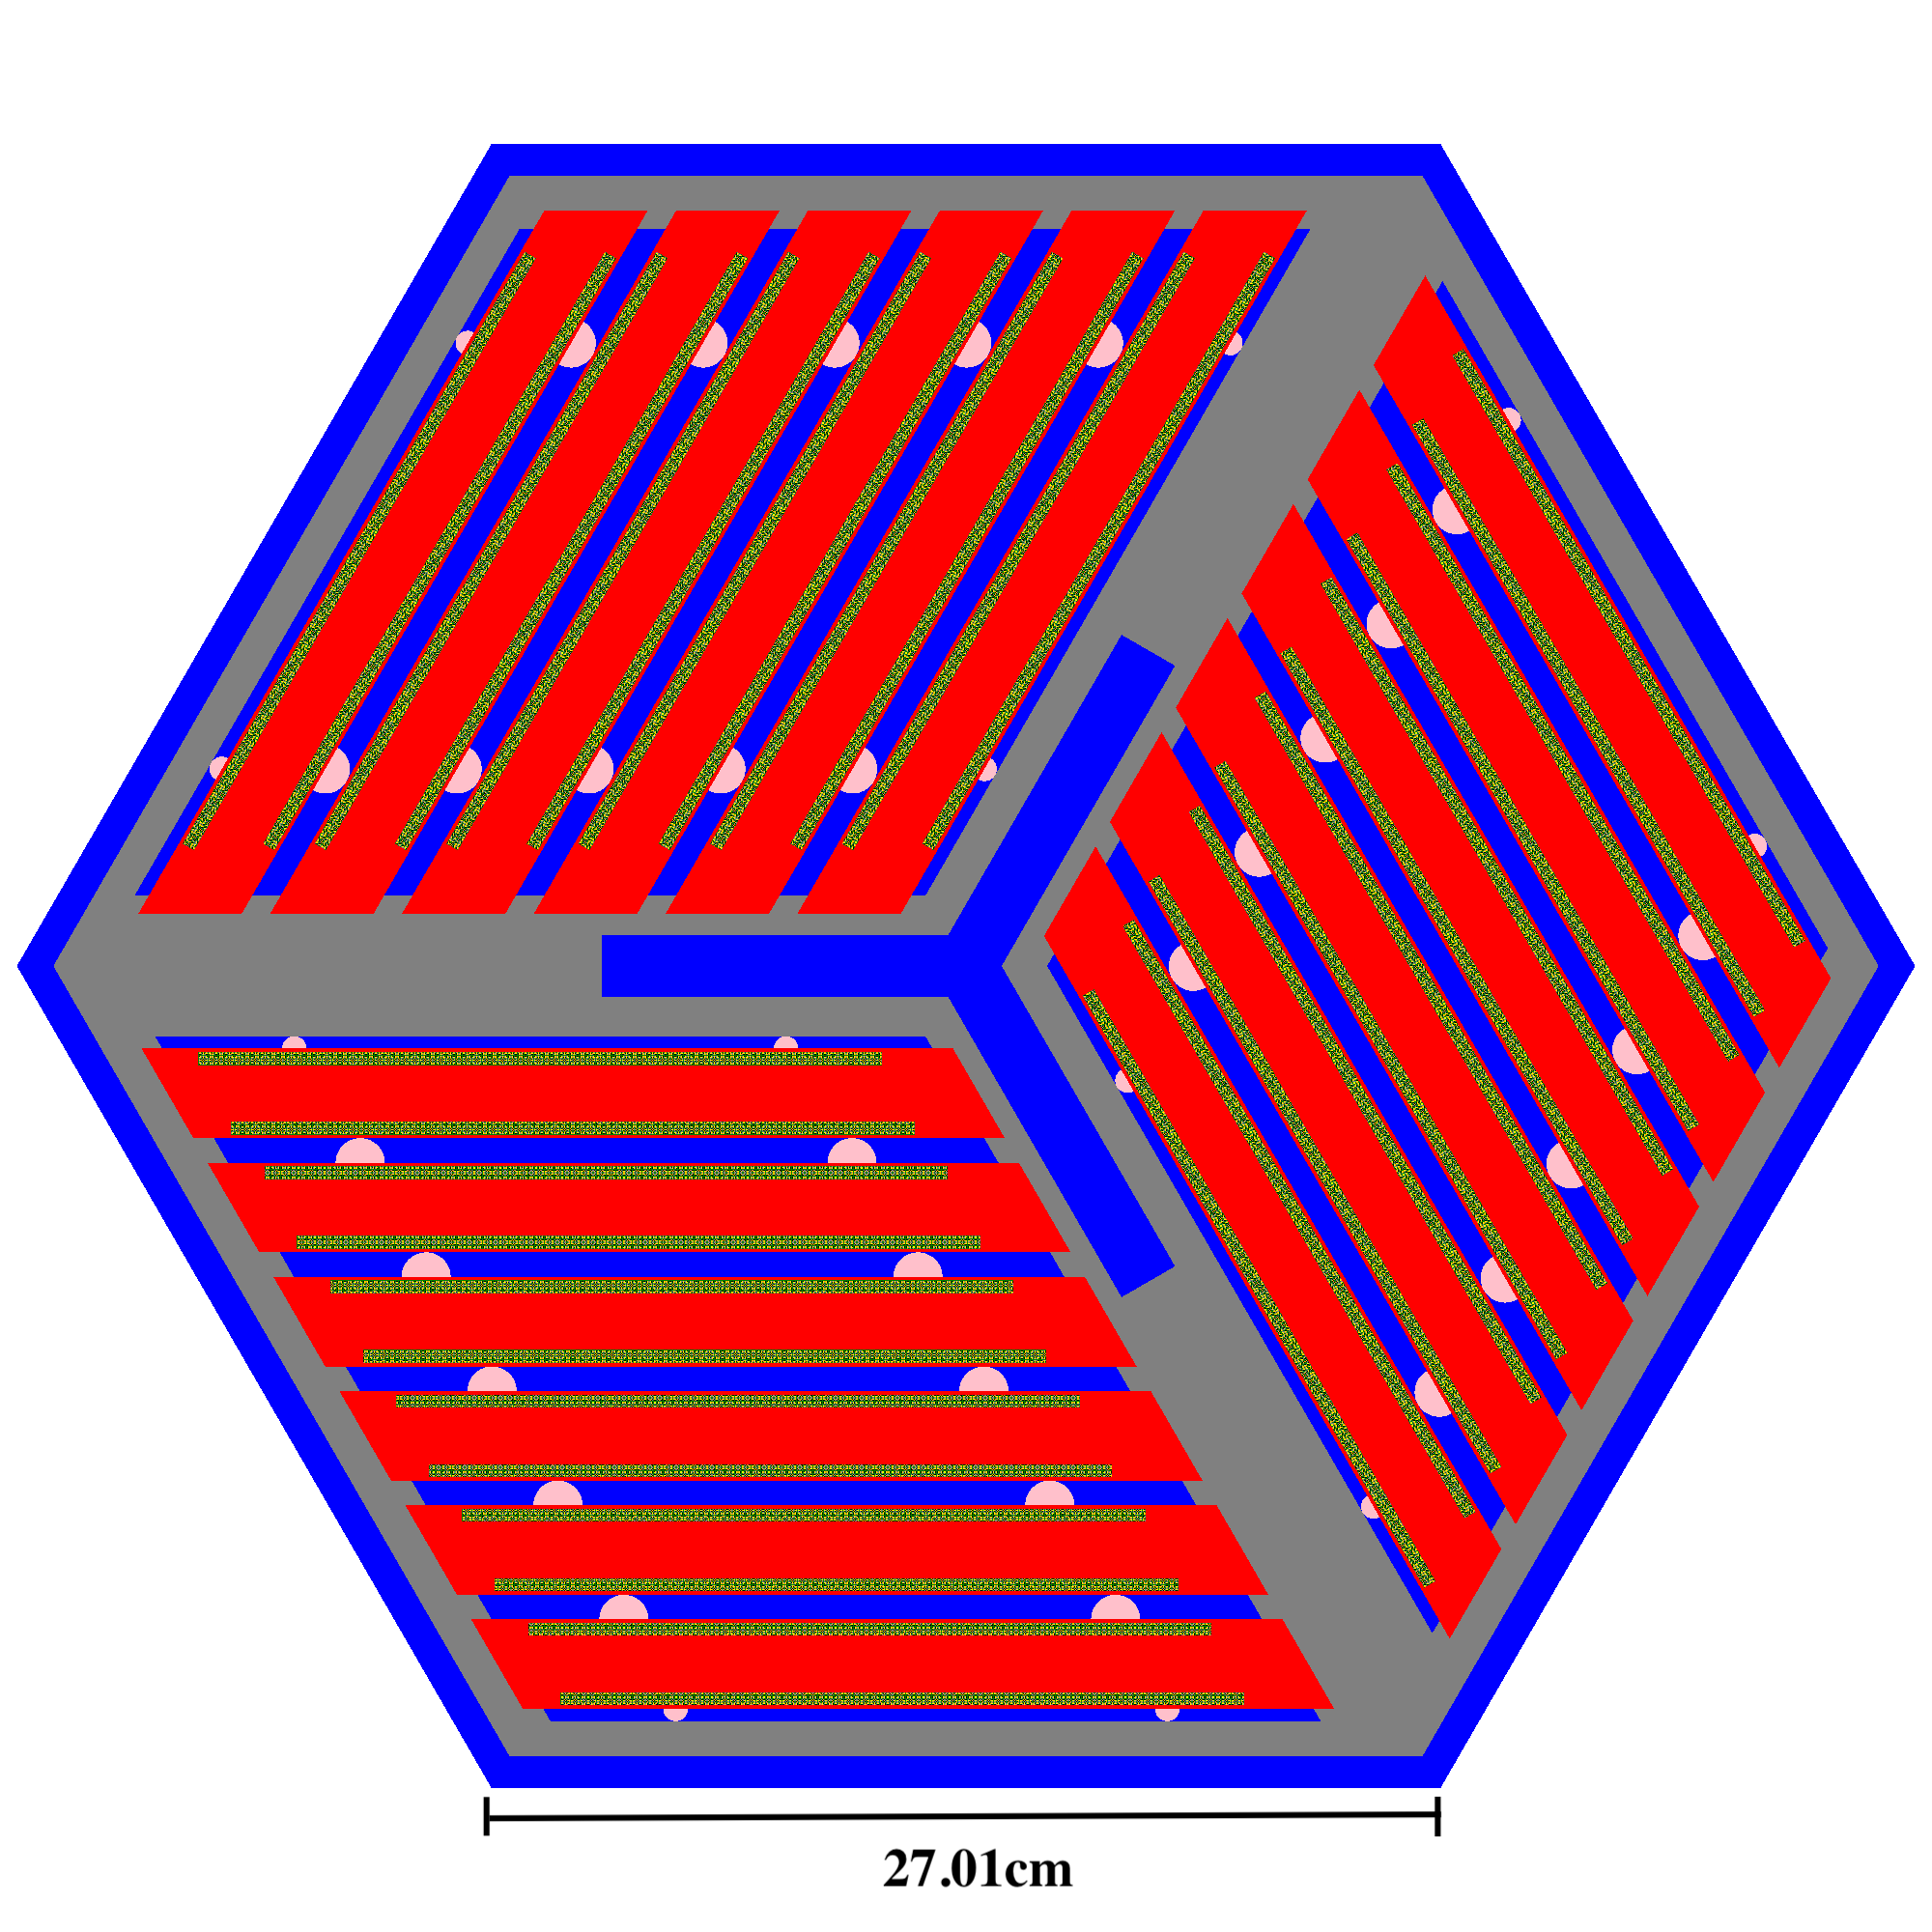
\includegraphics[width=0.6\linewidth]{../docs/figures/ahtr-fuel-element.png}} 
        \only<2>{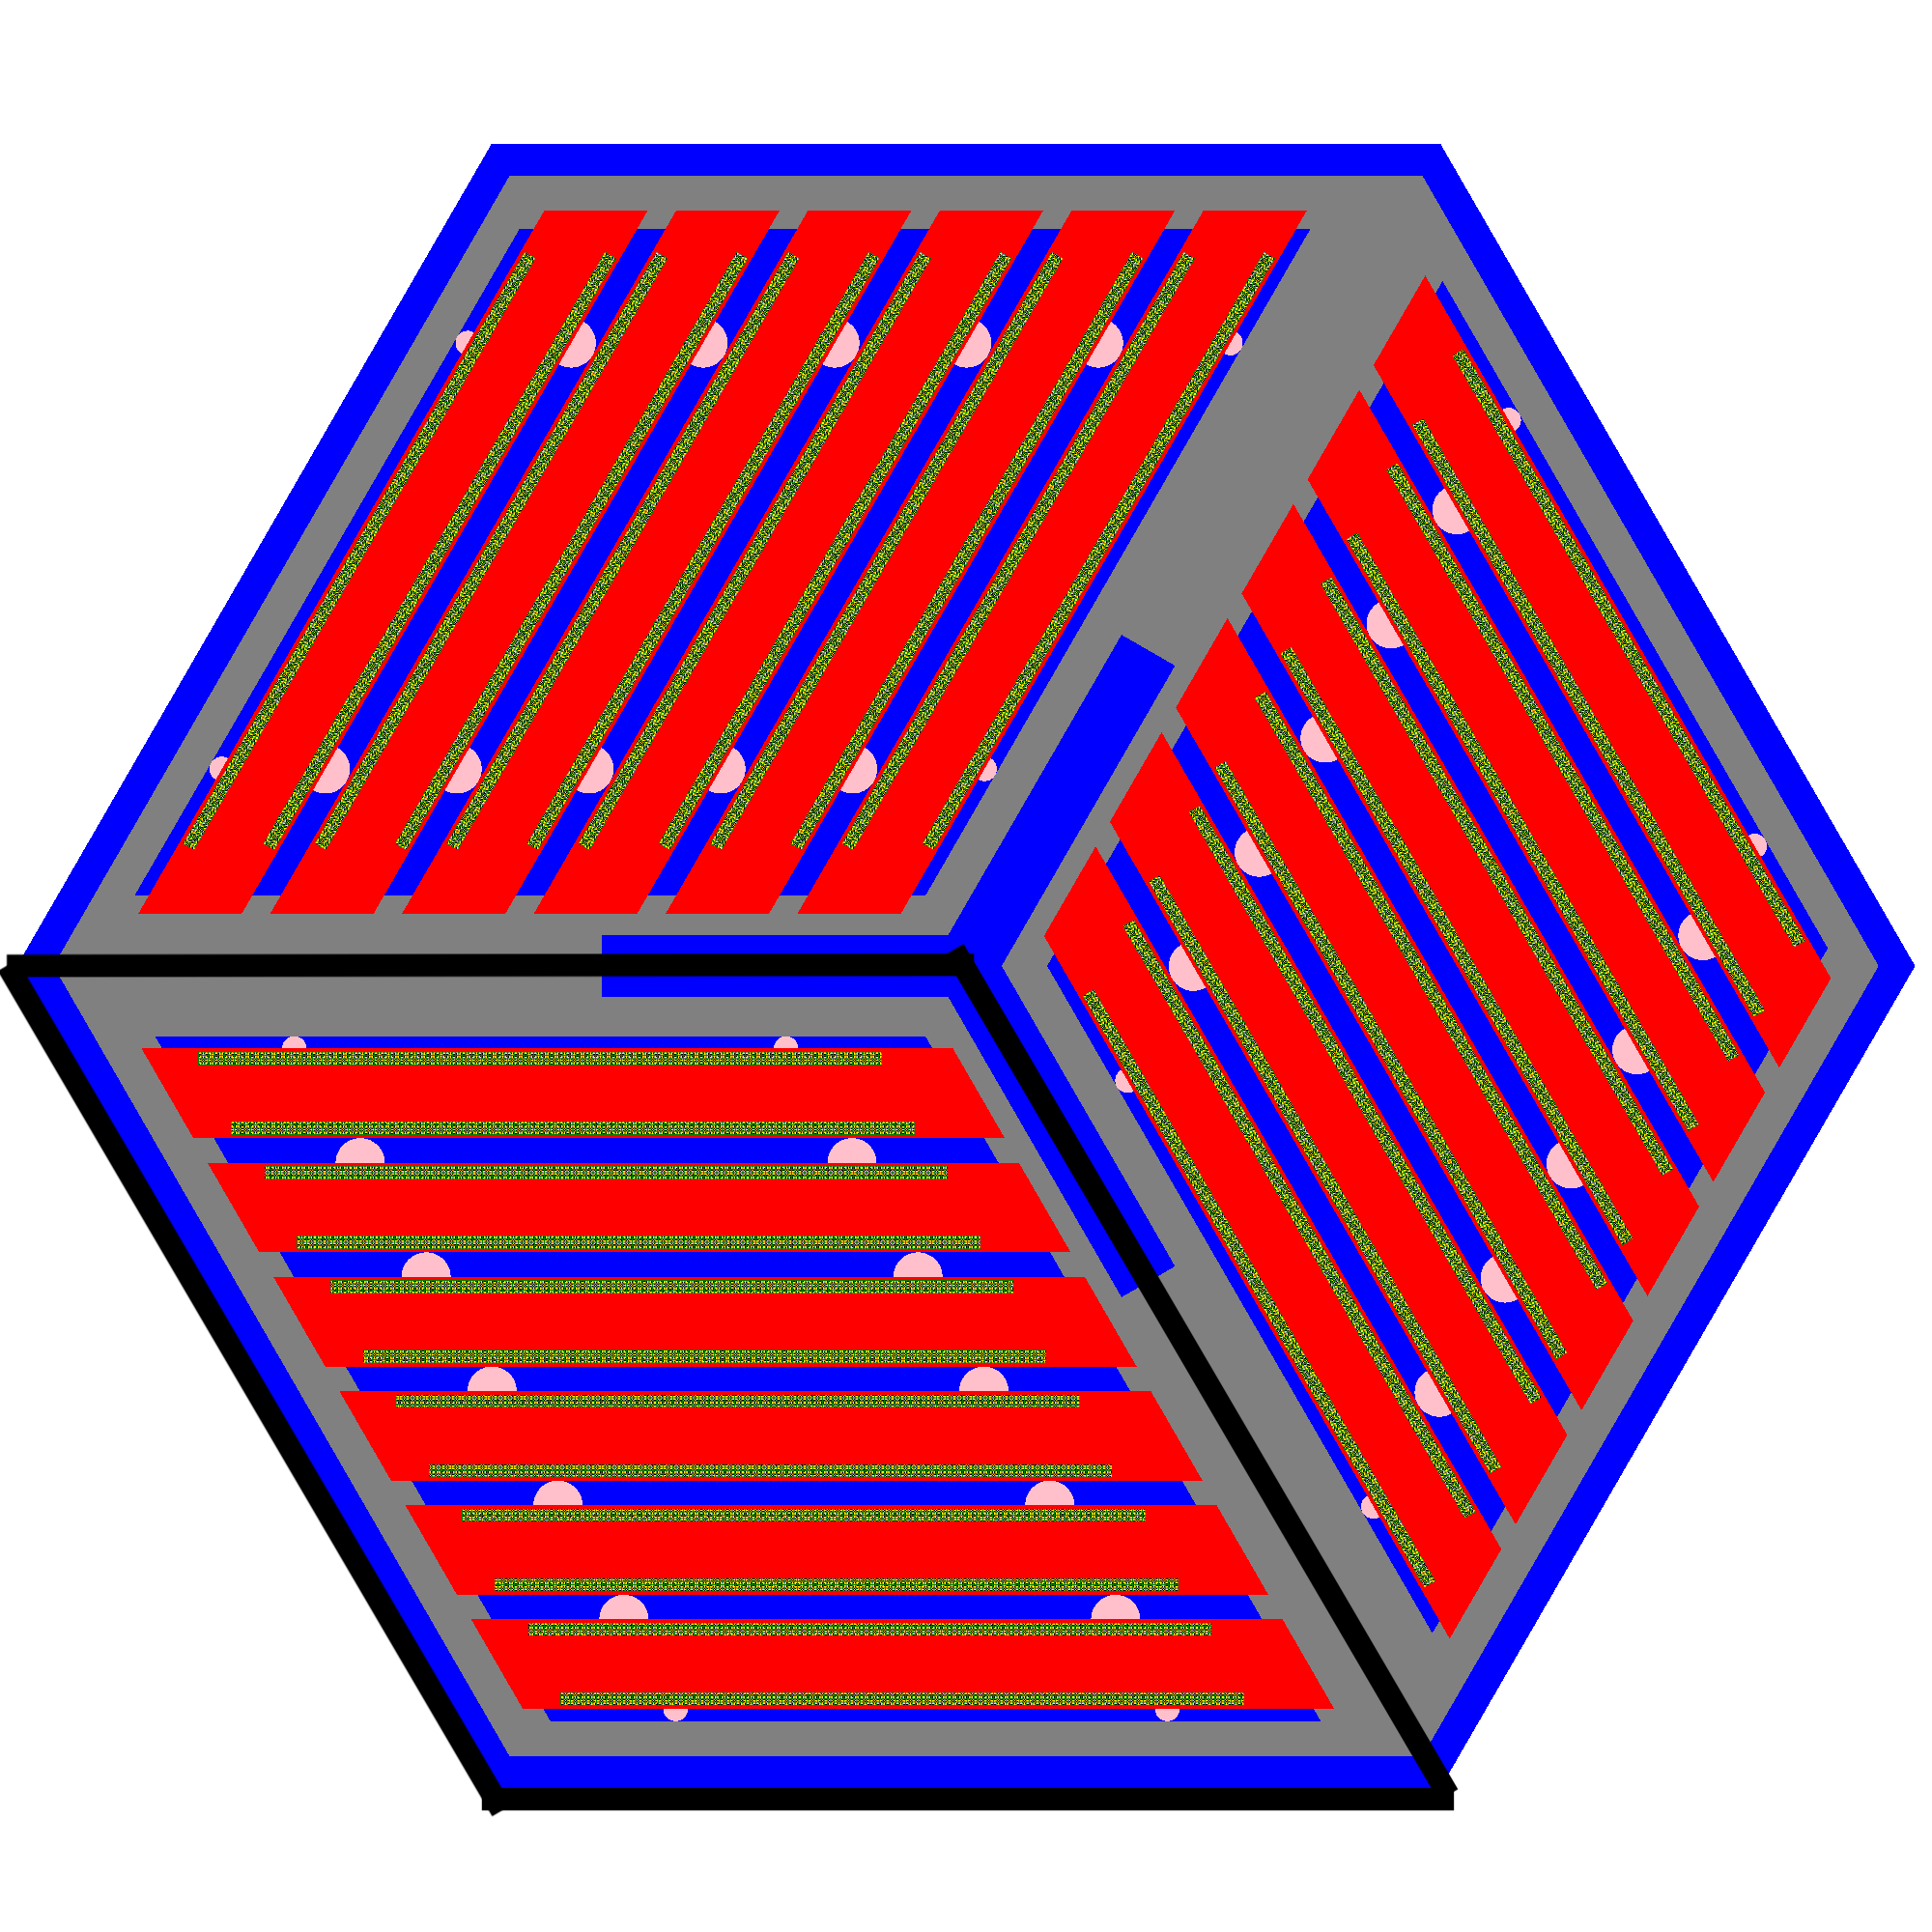
\includegraphics[width=0.6\linewidth]{figures/ahtr-fuel-element-annotated.png}} 
    \end{figure}
\end{frame}

\begin{frame}
    \frametitle{AHTR One-Third Assembly Geometry}
    \visible<1->{\textbf{Two sine distributions govern TRISO packing fraction distribution:}
    \begin{align}
    \rho_{TRISO}(\vec{x}, \vec{y}) &= \left(\textbf{a}\cdot sin(\textbf{b}\cdot 
    x + \textbf{c}) + 2\right) \cdot \left(\textbf{d}\cdot sin(\textbf{e}\cdot y + 
    \textbf{f}) + 2\right) \cdot NF \nonumber
    \end{align}
    
    The normalization factor (NF) ensures that total amount of TRISO particles in the 
    one-third assembly equals to $PF_{total}$.}

    \vspace{-0.3cm}
    \begin{columns}[t]
        \begin{column}{0.5\textwidth}
        \begin{figure}
            \only<1-2>{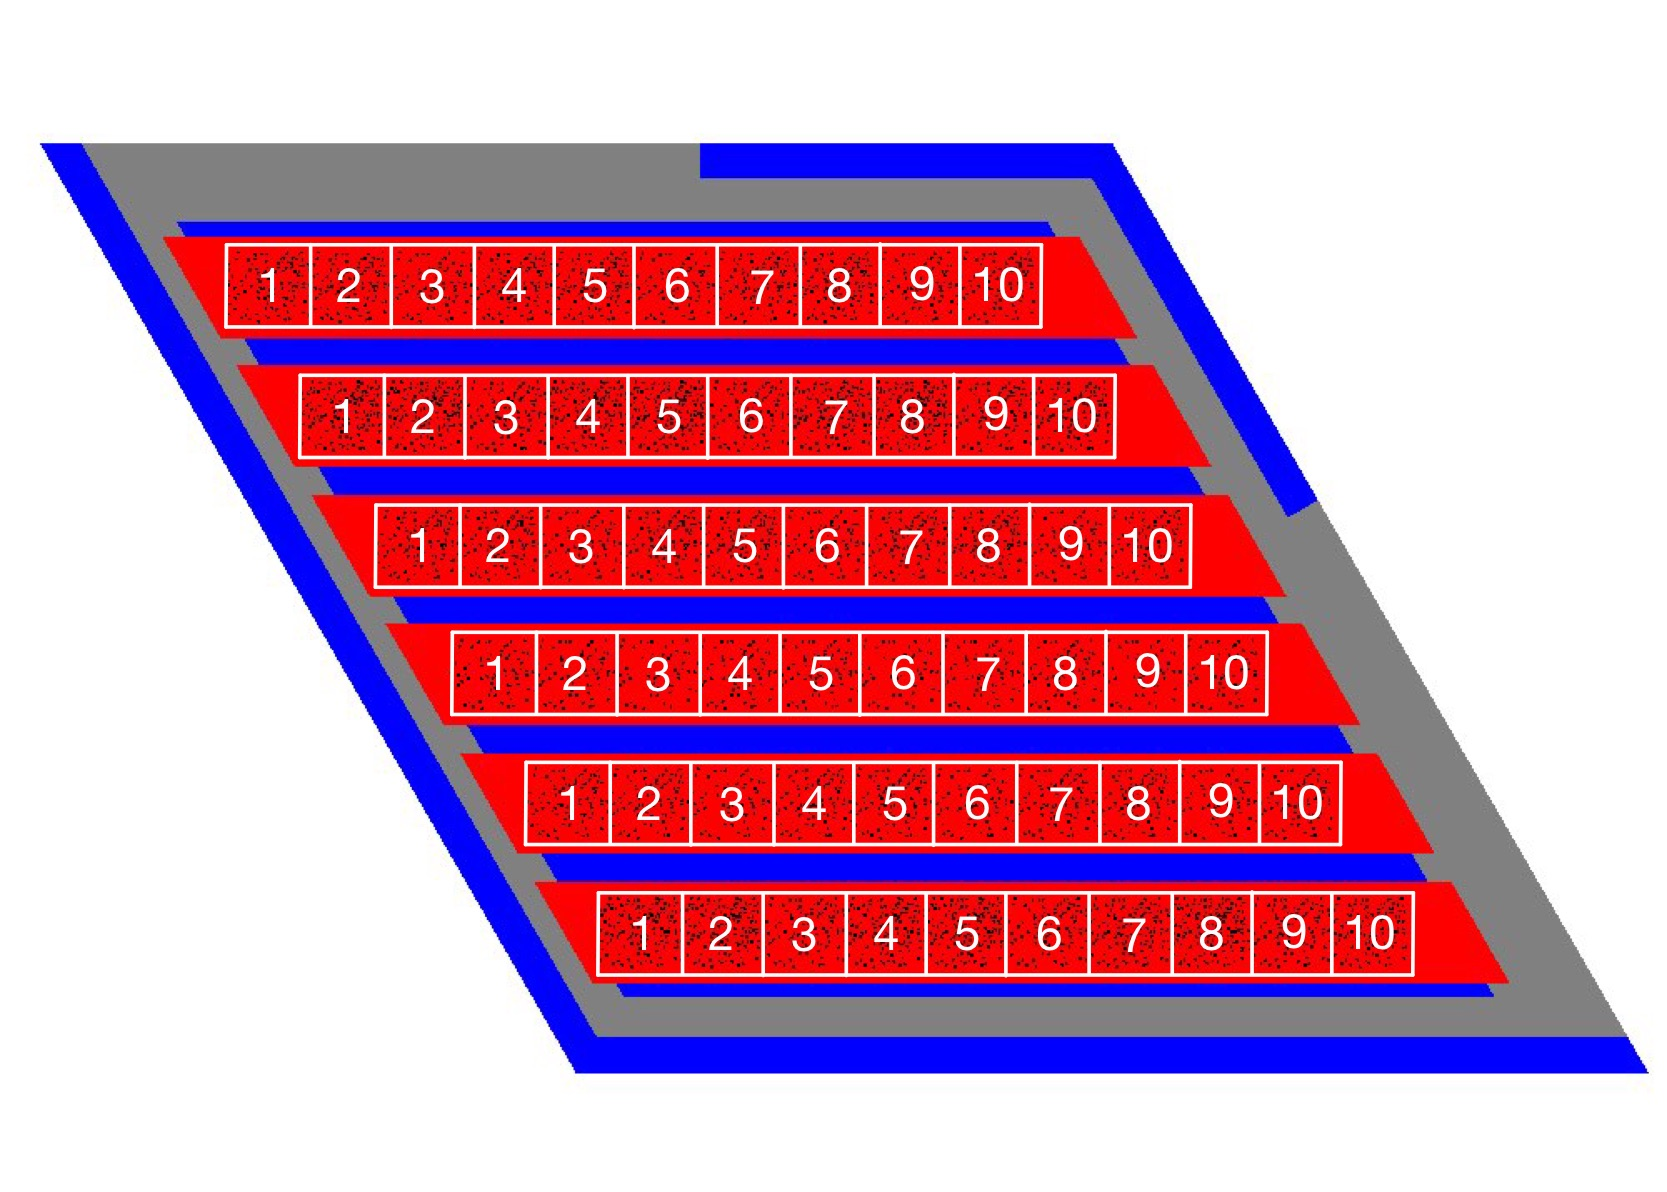
\includegraphics[width=\linewidth]{../docs/figures/ahtr_assembly.png} 
            \vspace{-0.6cm}
            \caption{AHTR one-third assembly illustrating packing fraction discretization.}}
            \only<3>{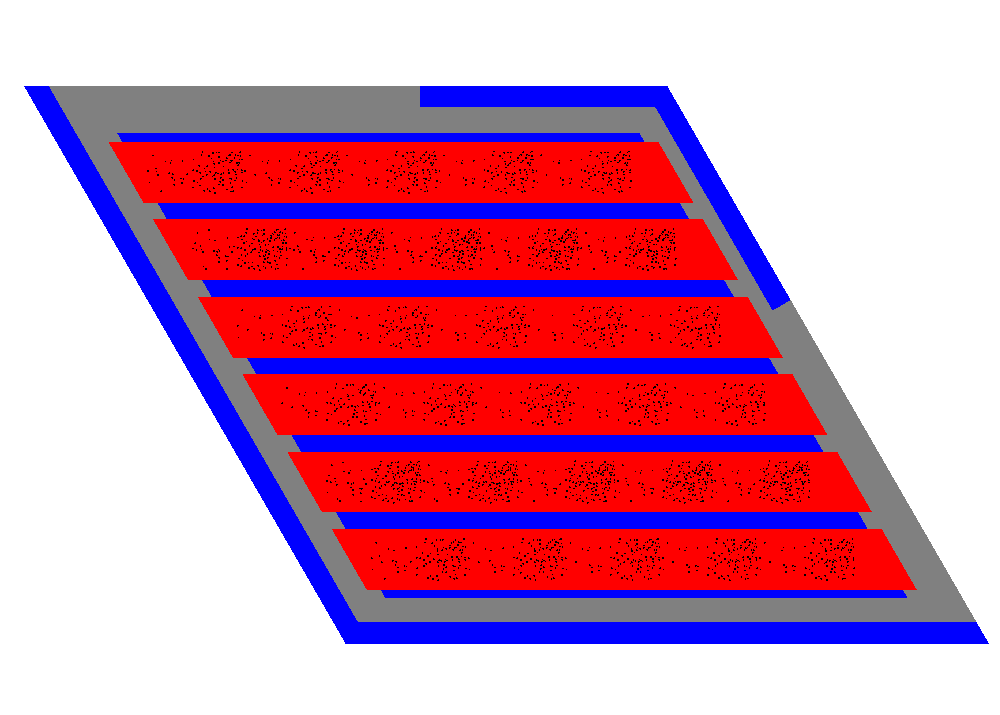
\includegraphics[width=\linewidth]{../docs/figures/assem-obj-1-pf-most-minimized.png} 
            \vspace{-0.6cm}
            \caption{AHTR one-third assembly illustrating packing fraction variation.}}
        \end{figure}
        \end{column}
        \begin{column}{0.5\textwidth} 
            \visible<2->{\begin{figure}
                \textbf{a} = 1.435, \textbf{b} = 1.488, \textbf{c} = 2.362, \\
                \textbf{d} = 0.689, \textbf{e} = 0.584, \textbf{f} = 4.170
                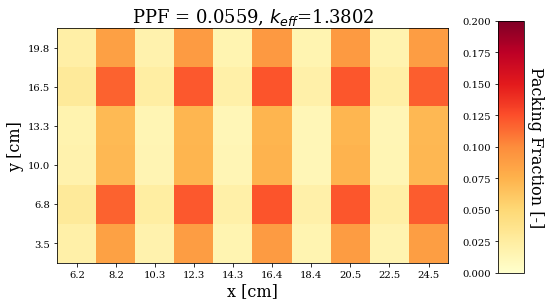
\includegraphics[width=\linewidth]{../docs/figures/assem-0.0559-most-minimized.png} 
                \caption{TRISO distribution example.}
            \end{figure}}
        \end{column}
        \end{columns}
\end{frame}

\begin{frame}
    \frametitle{Contd. AHTR One-Third Assembly Geometry}
    \textbf{Five radius values (\textbf{$r_1, r_2, r_3, r_4, r_5$}) 
    control coolant channel shape.}
    \begin{figure}
        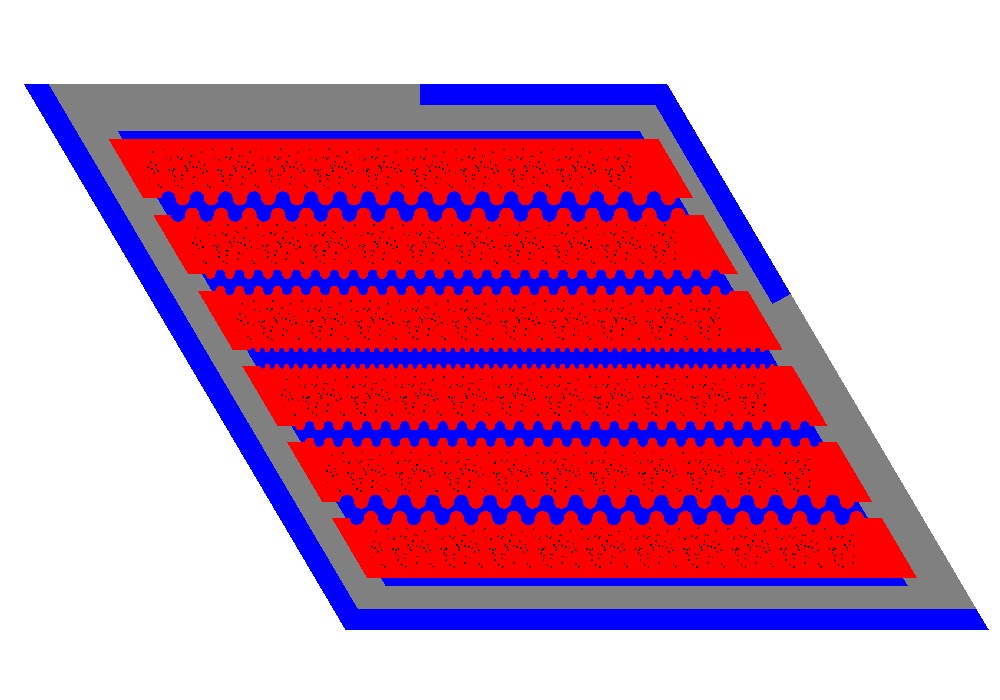
\includegraphics[width=0.7\linewidth]{../docs/figures/coolant-channel-shape-assem.png} 
        \vspace{-0.3cm}
        \caption{AHTR one-third assembly with coolant channel shape variation, 
        $r_1, r_2, r_3, r_4, r_5$ = 0.3cm, 0.2cm, 0.1cm, 0.2cm, 0.3cm.}
    \end{figure}
\end{frame}

\begin{frame}
    \frametitle{ROLLO AHTR Optimization Workflow}
    \vspace{-0.2cm}
    \begin{figure}
        \makebox[\textwidth][c]{
            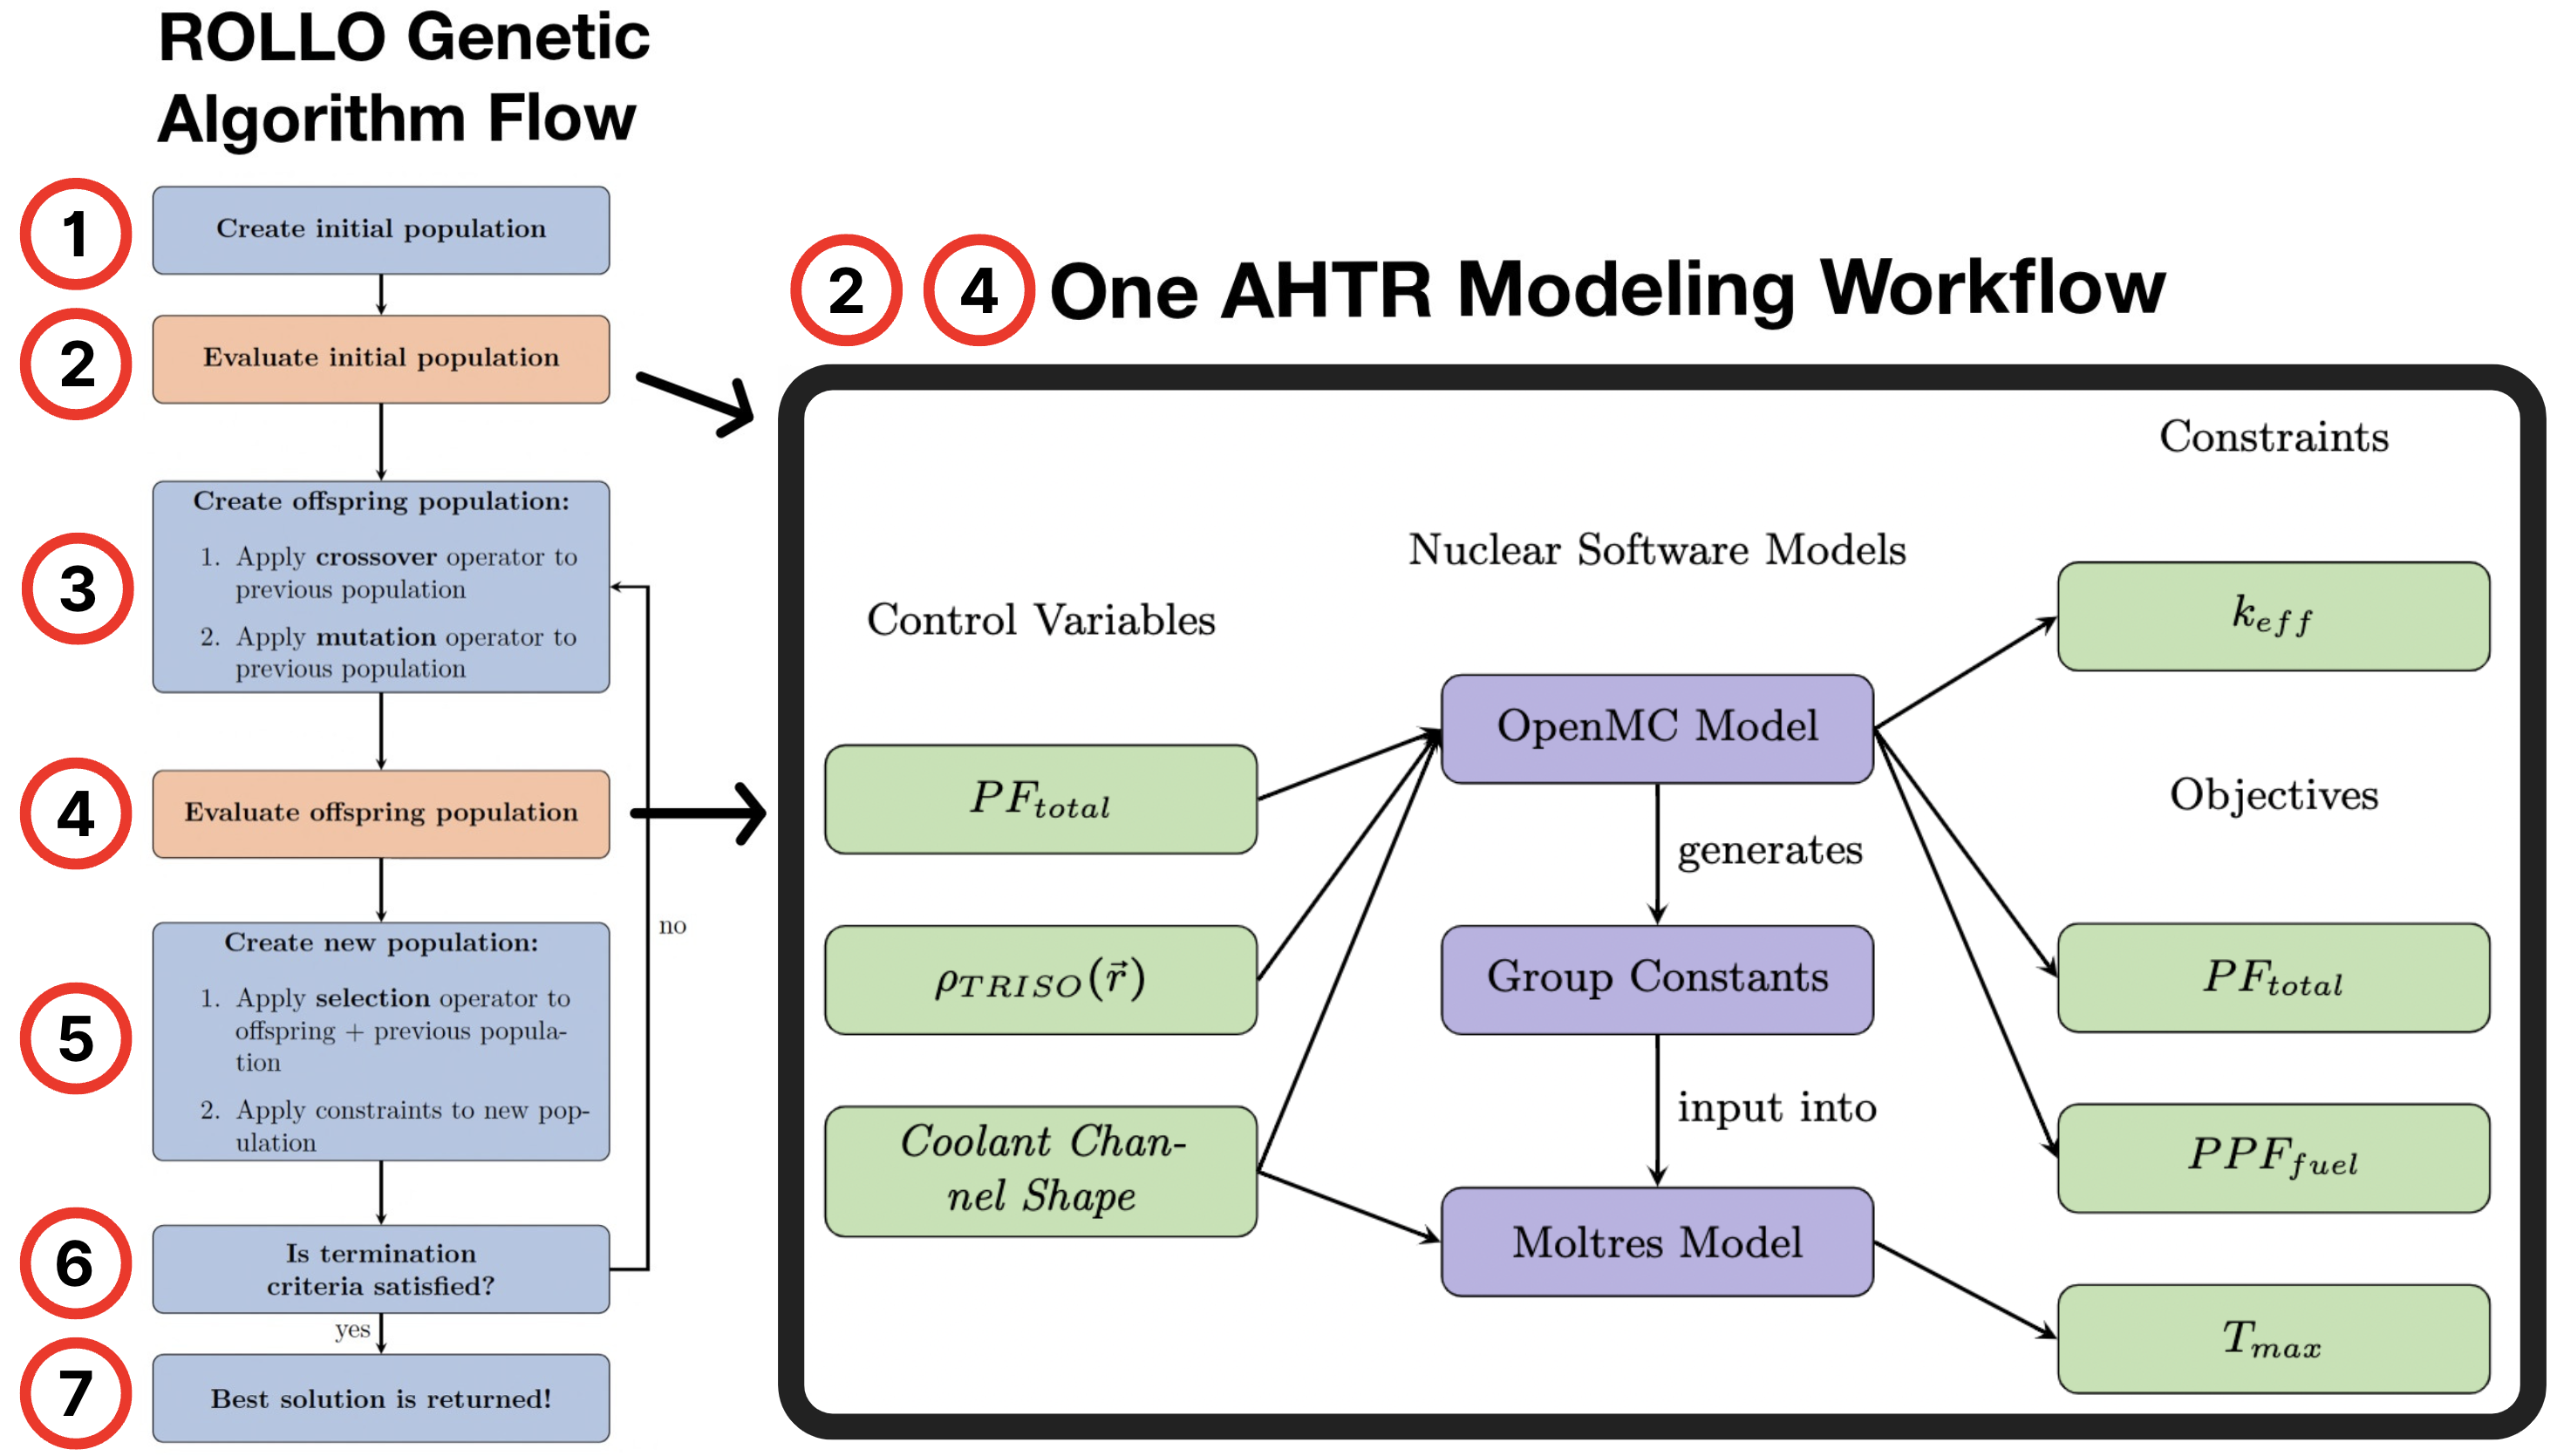
\includegraphics[width=1.1\linewidth]{figures/ahtr-modeling-workflow-numbered.png}} 
        %\caption{ROLLO AHTR Optimization Workflow.}
    \end{figure}
\end{frame}

\subsection{AHTR One-Third Assembly Optimization Results}
\begin{frame}
    \frametitle{AHTR One-Third Assembly Optimization Simulations}
    \only<1>{
        \vspace{-0.2cm}
        \begin{figure}
            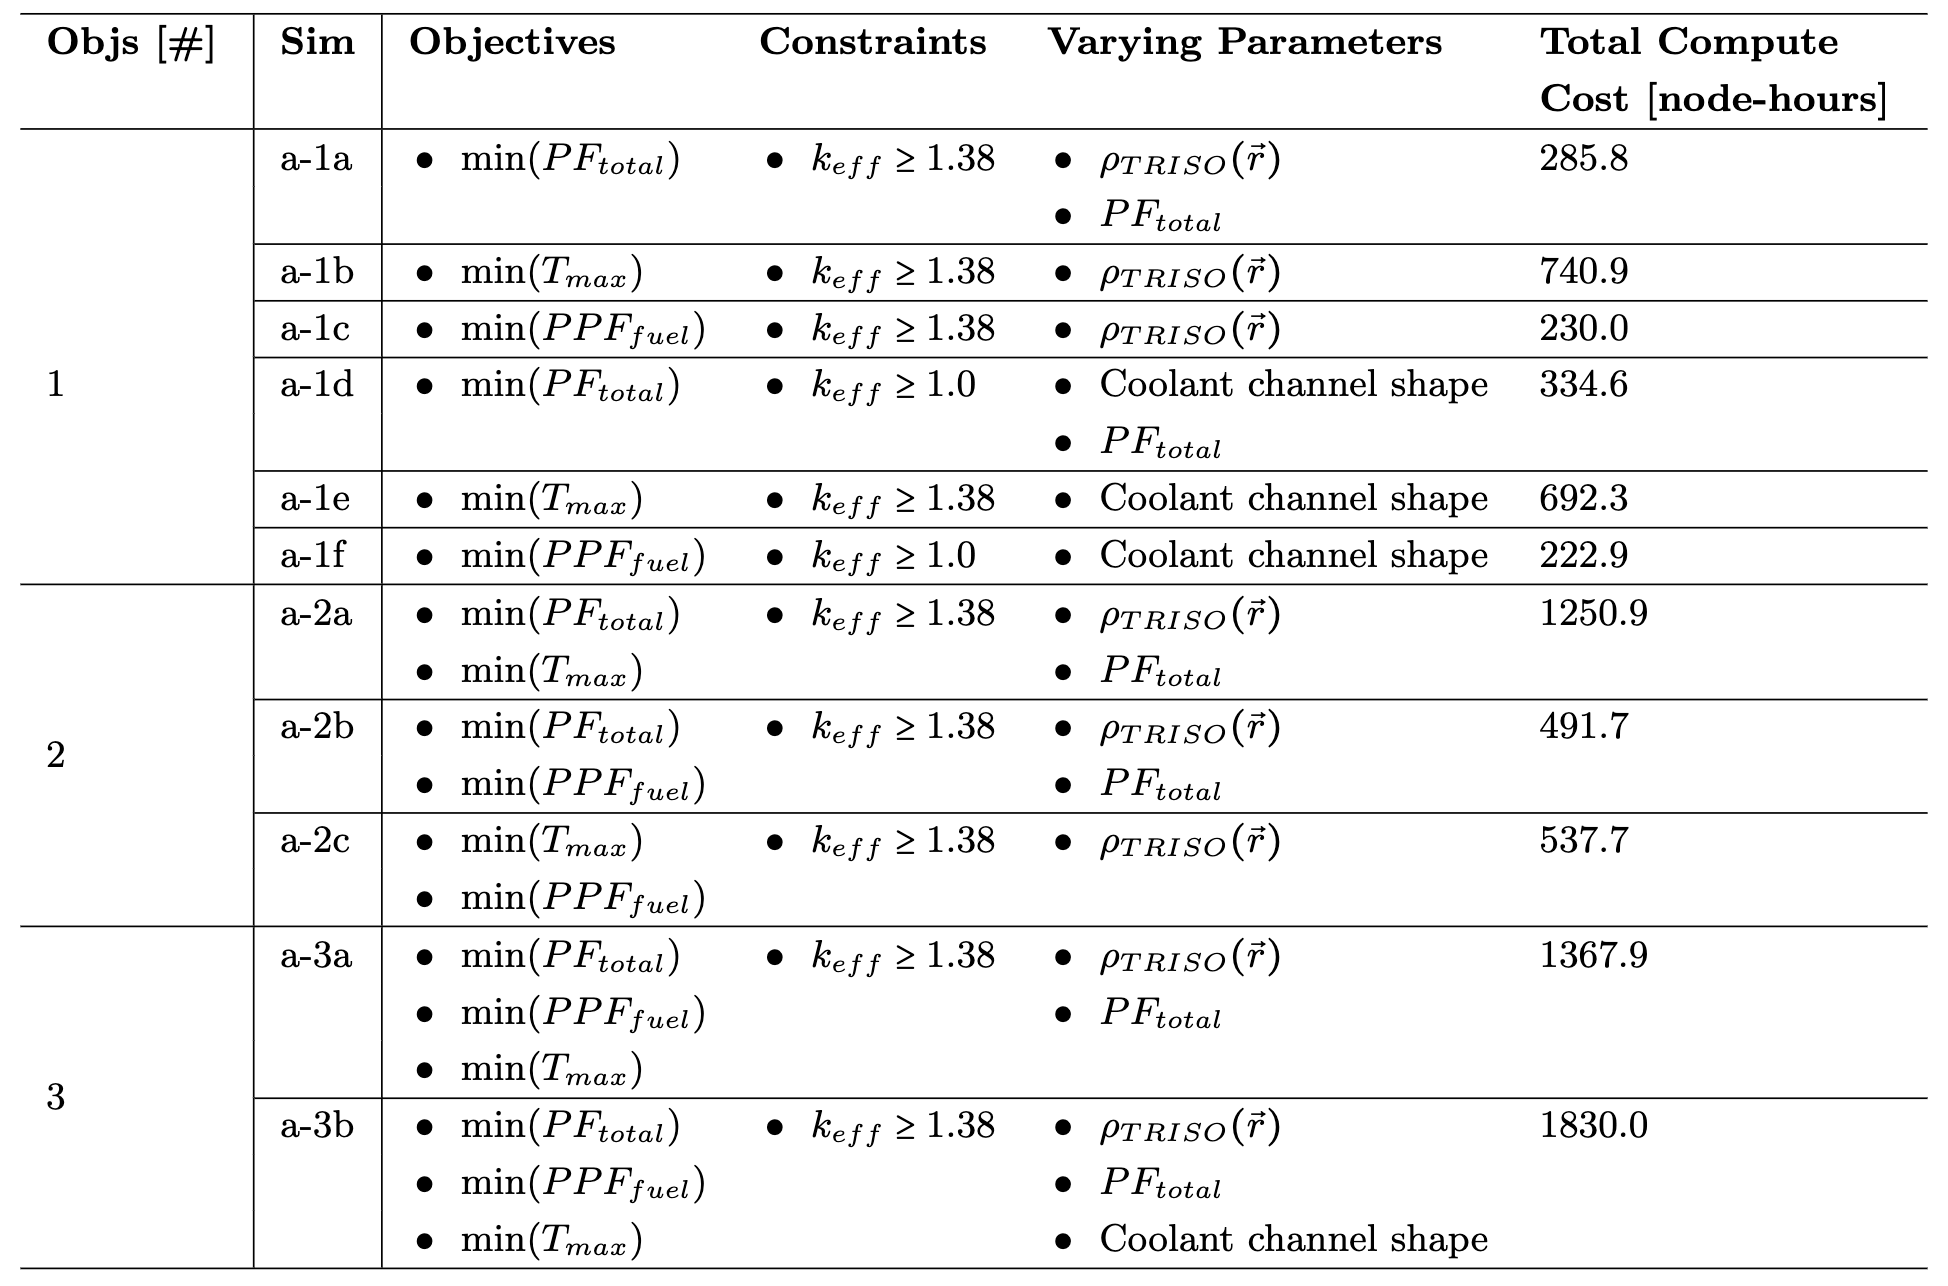
\includegraphics[width=0.8\linewidth]{figures/ahtr-assem-opt-table.png}
        \end{figure}

        \vspace{-0.2cm}
        \textbf{All the optimization simulations are run on the Theta supercomputer} 
        at the Argonne Leadership Computing Facility \cite{noauthor_thetathetagpu_2022}.

        Each Theta node has 64 1.3-GHz Intel Xeon Phi 7230 processors.
        }

        \only<2>{
            \begin{figure}
                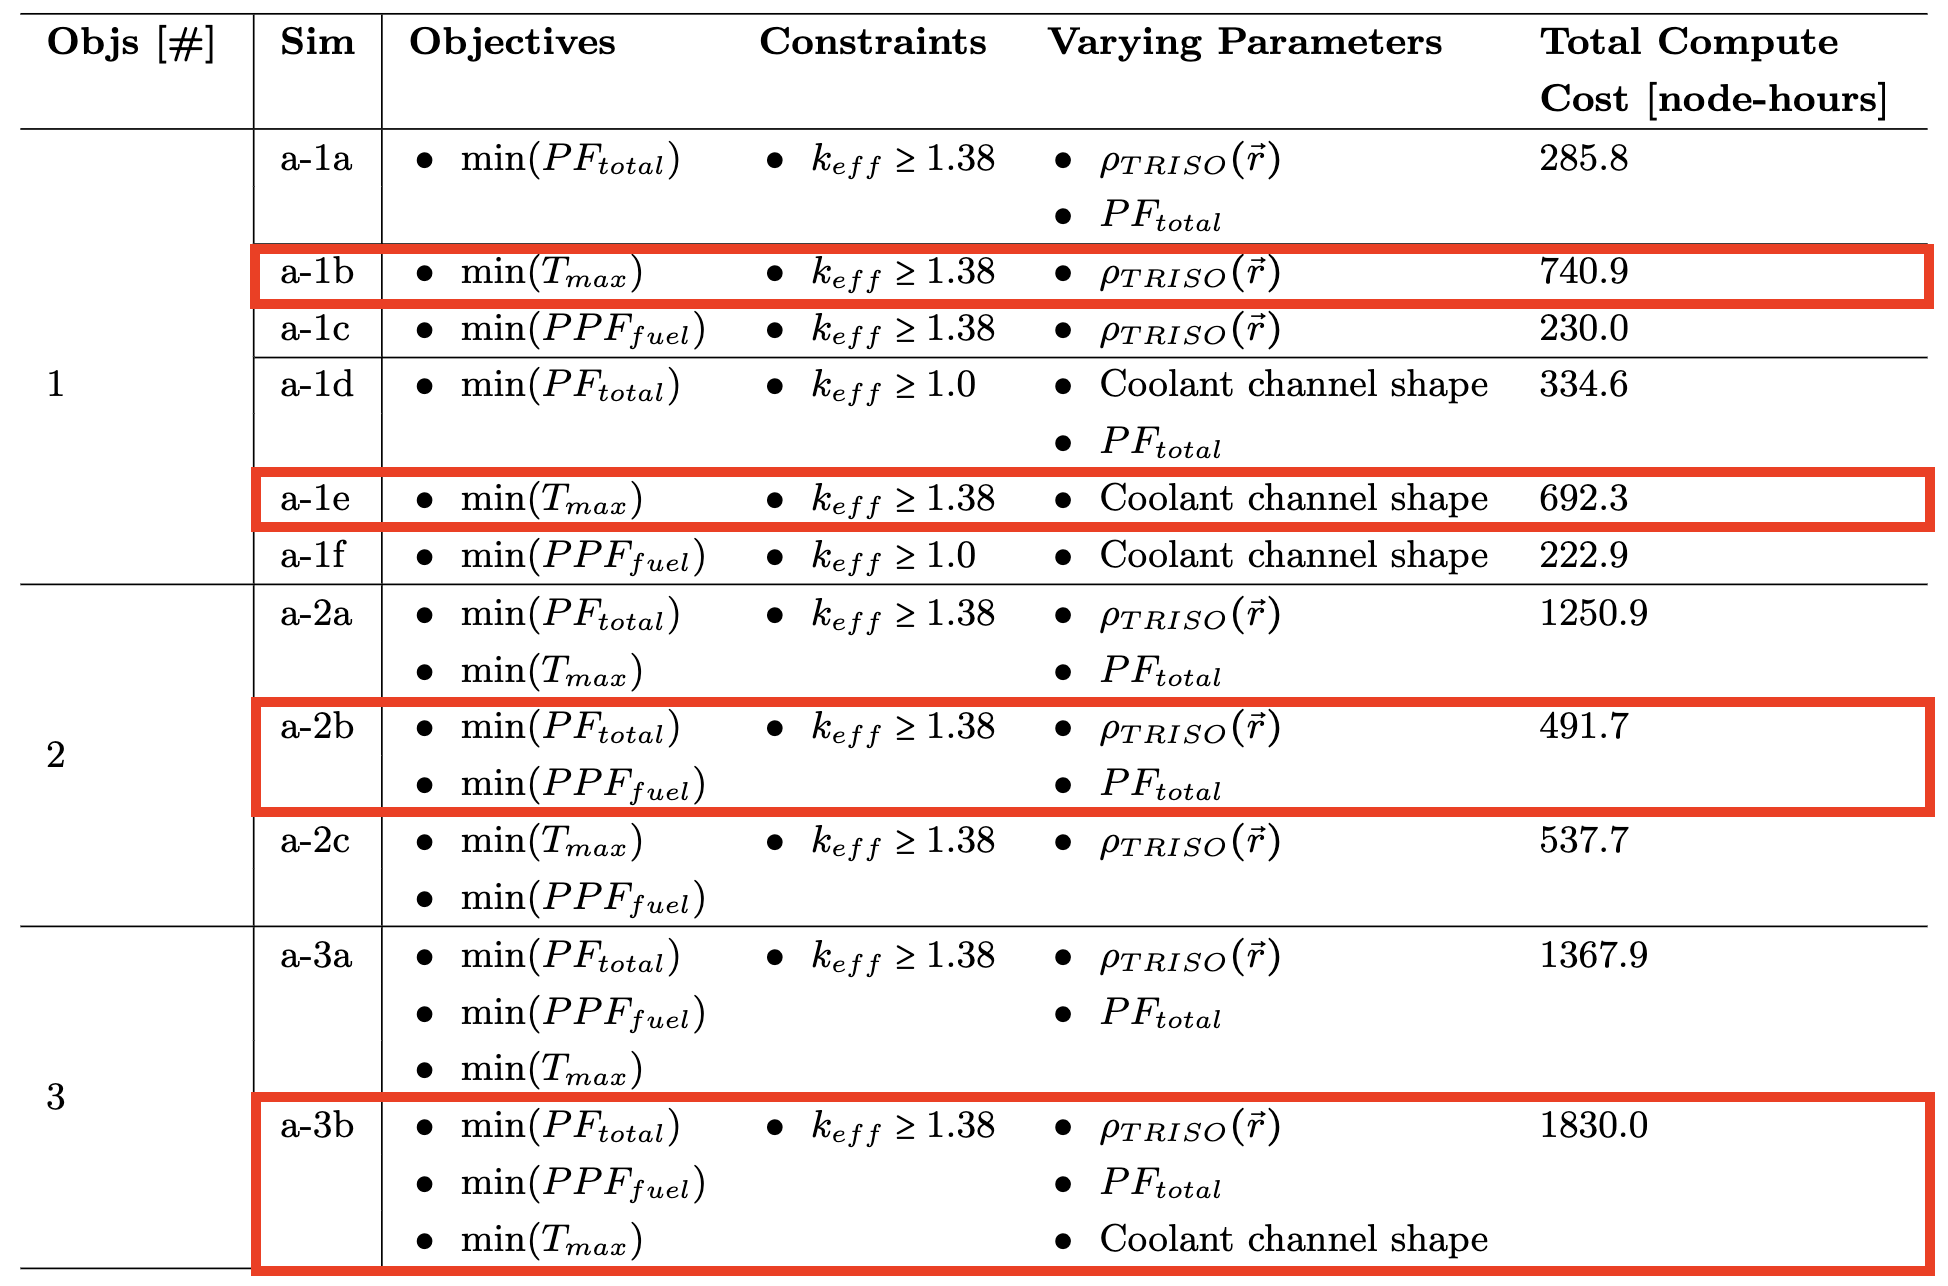
\includegraphics[width=0.9\linewidth]{figures/ahtr-assem-opt-table-annotated.png}
            \end{figure}}

        \only<3>{
            \begin{figure}
                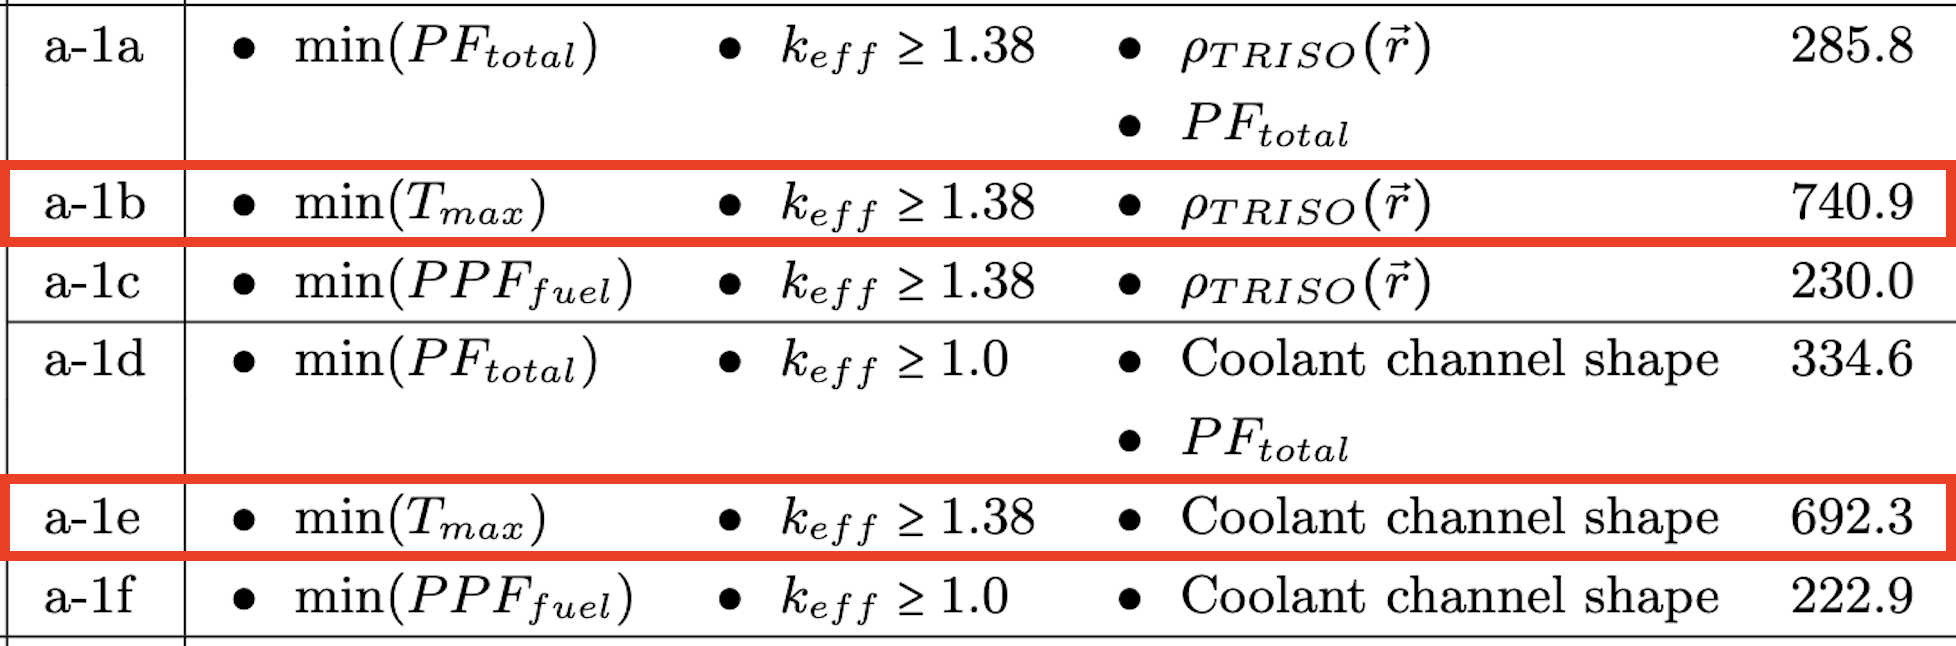
\includegraphics[width=\linewidth]{figures/ahtr-assem-opt-table-annotated1.png}
            \end{figure}
    
            Simulations a-1b and a-1e demonstrate \textbf{how the input parameters 
            $\rho_{TRISO}(\vec{r})$ and coolant channel shape respond to 
            the minimize $T_{max}$ objective}.

            \vspace{0.2cm}
            I constrained $k_{eff} \geq 1.38$ find optimal input parameters 
            that achieve \textbf{similar performance to the FHR benchmark} TRISO distribution.}
        
        \only<4>{
            \begin{figure}
                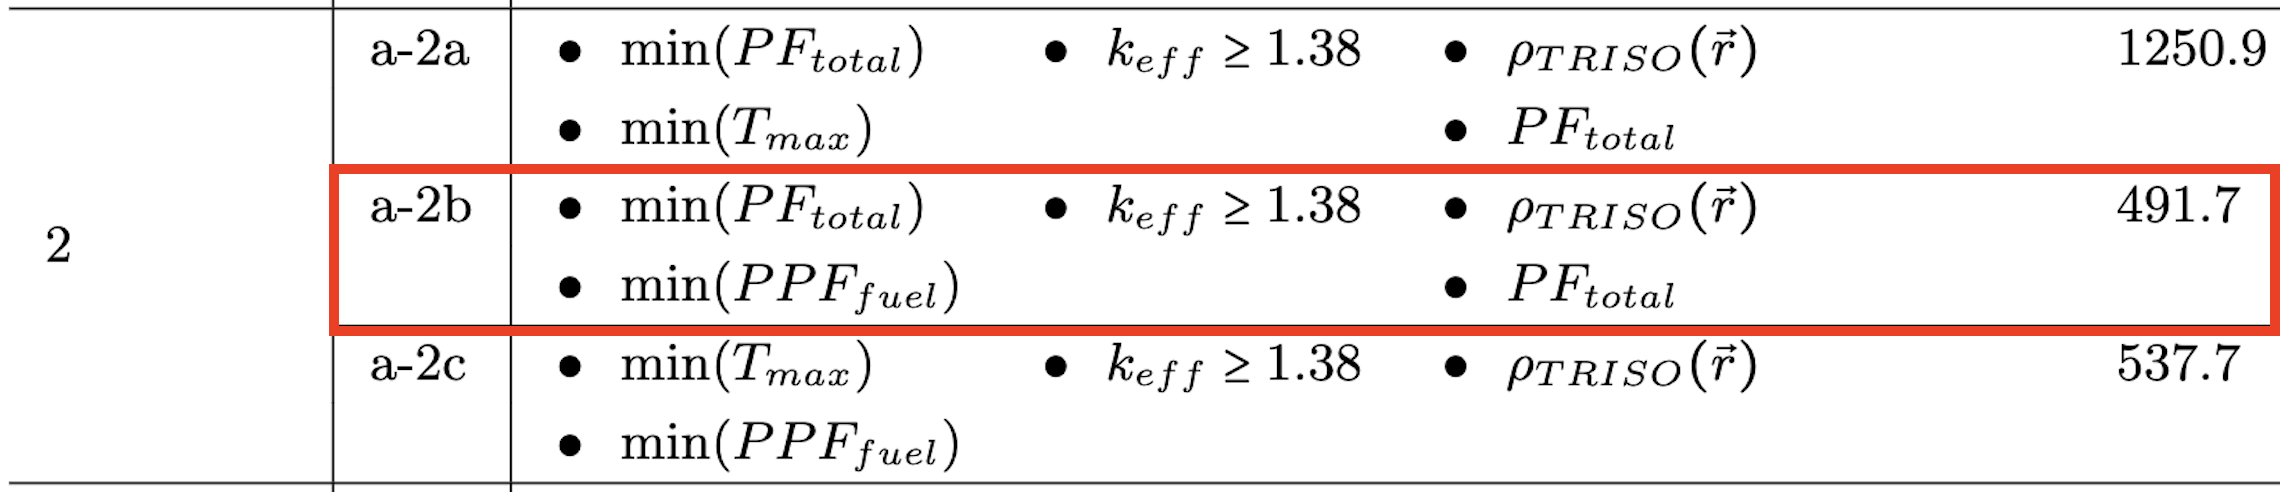
\includegraphics[width=\linewidth]{figures/ahtr-assem-opt-table-annotated2.png}
            \end{figure}

            Simulation a-2b demonstrates \textbf{how the input parameters $PF_{total}$ 
            and $\rho_{TRISO}(\vec{r})$ change as the minimize $PF_{total}$ and 
            $PPF_{fuel}$ objectives interact}.
        }

        \only<5>{
            \begin{figure}
                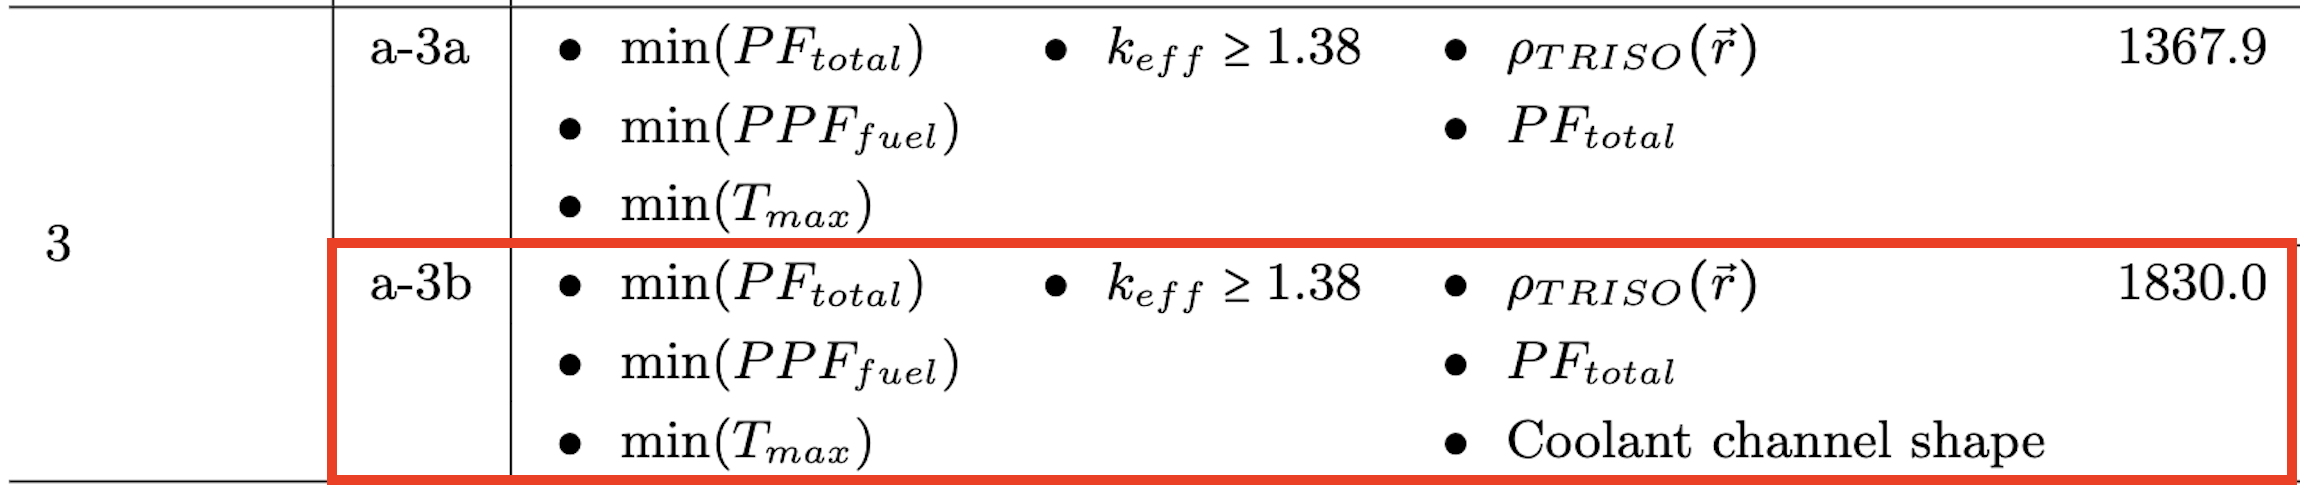
\includegraphics[width=\linewidth]{figures/ahtr-assem-opt-table-annotated3.png}
            \end{figure}

            Simulation a-3b is the \textbf{final and largest optimization problem} run 
            for the one-third assembly model that varies all input parameters to optimize 
            for all objectives. 
        }
    
\end{frame}

\begin{frame}
    \frametitle{AHTR One-Third Assembly Simulation a-1b Results}
    \visible<1->{\textbf{Simulation a-1b: I vary a, b, c, d, e f ($\rho_{TRISO}(\vec{x}, \vec{y})$)
    to minimize $T_{max}$.}} 

    \begin{figure}
        \only<1,4>{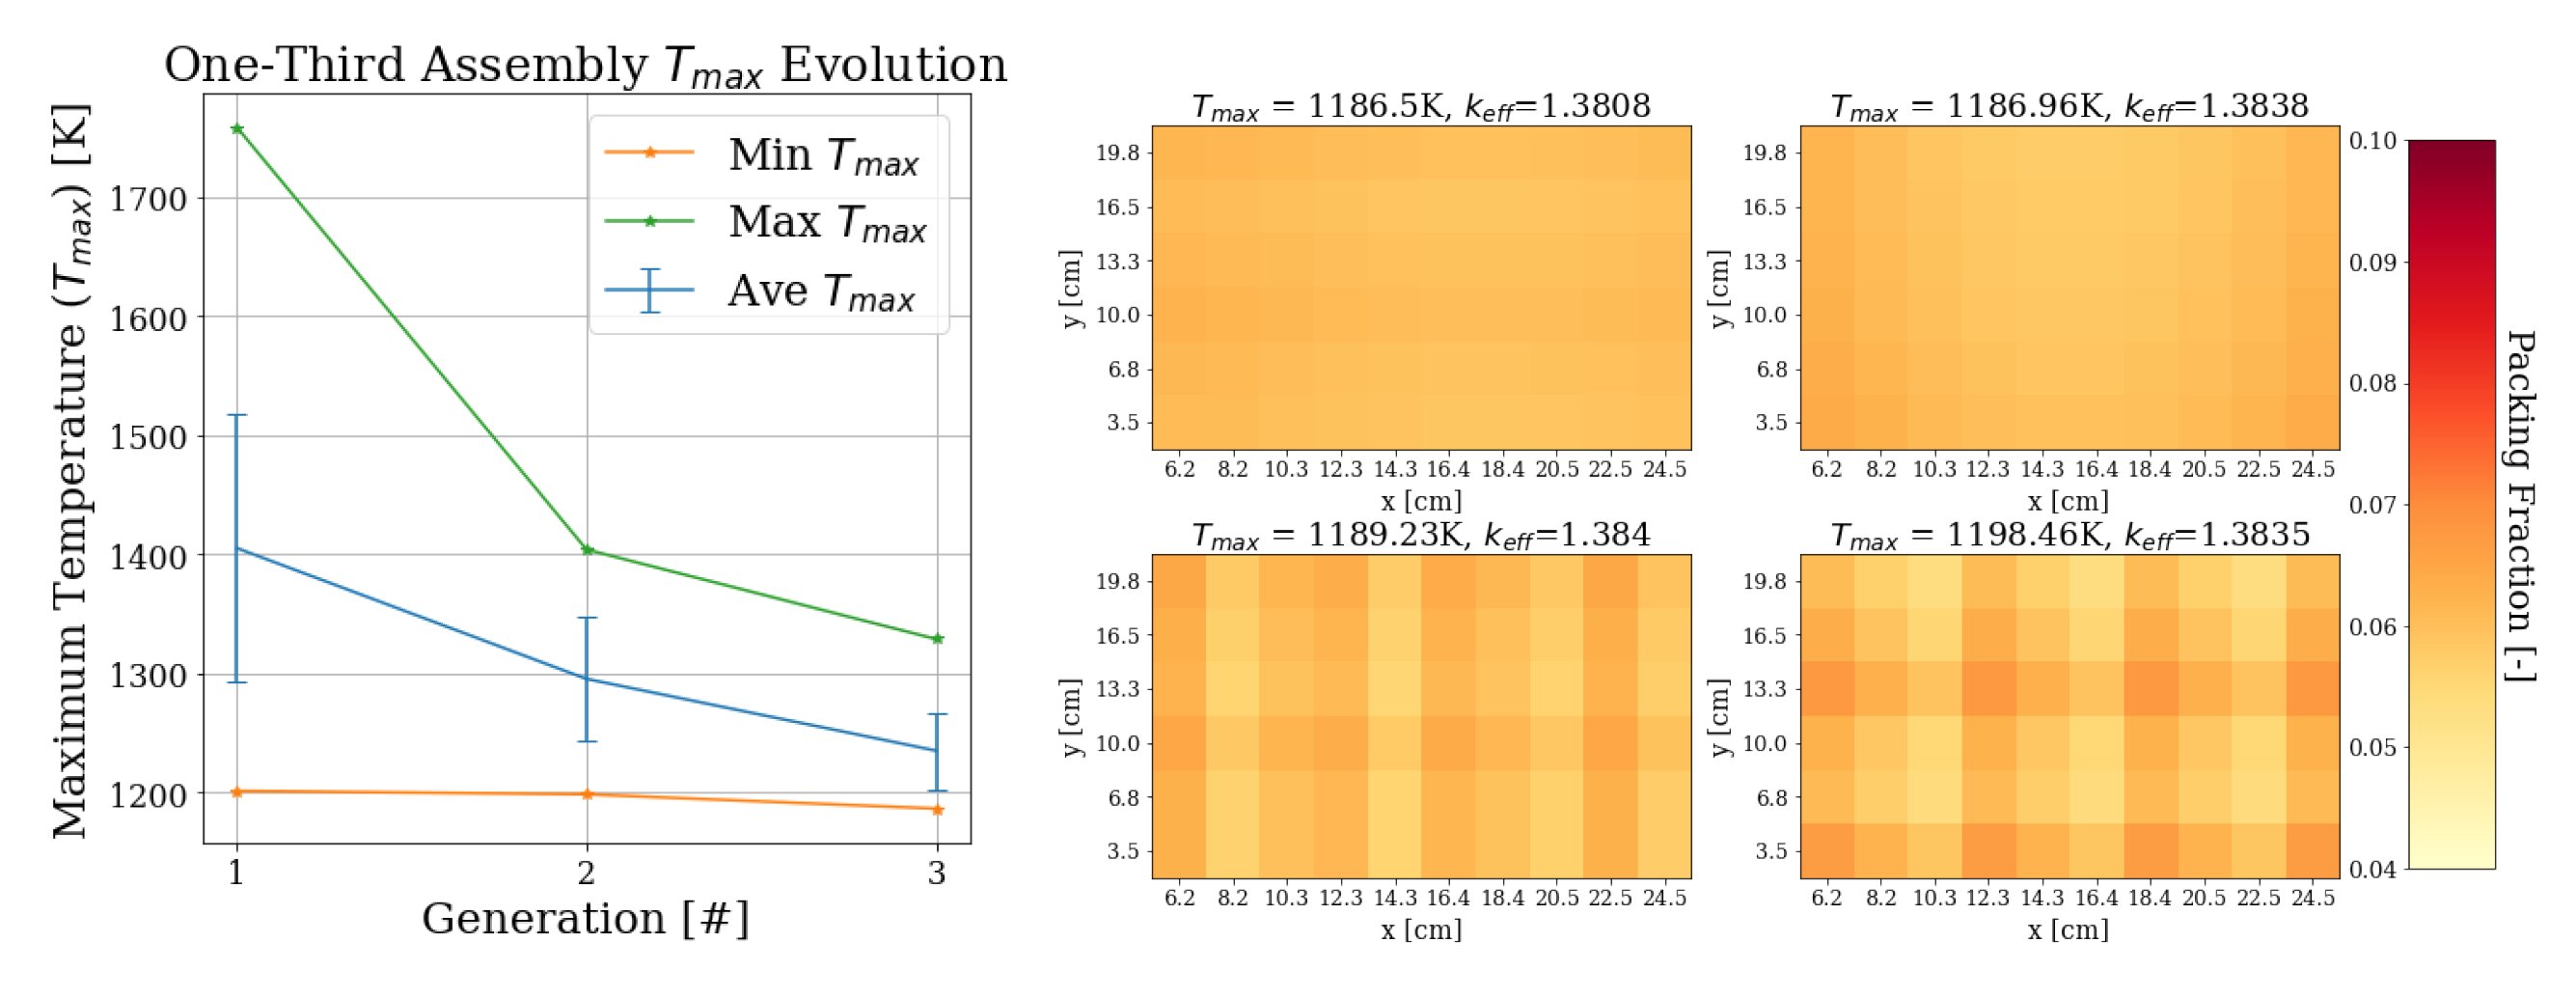
\includegraphics[width=\linewidth]{figures/assem-obj-1-temp.png}}
        \only<2>{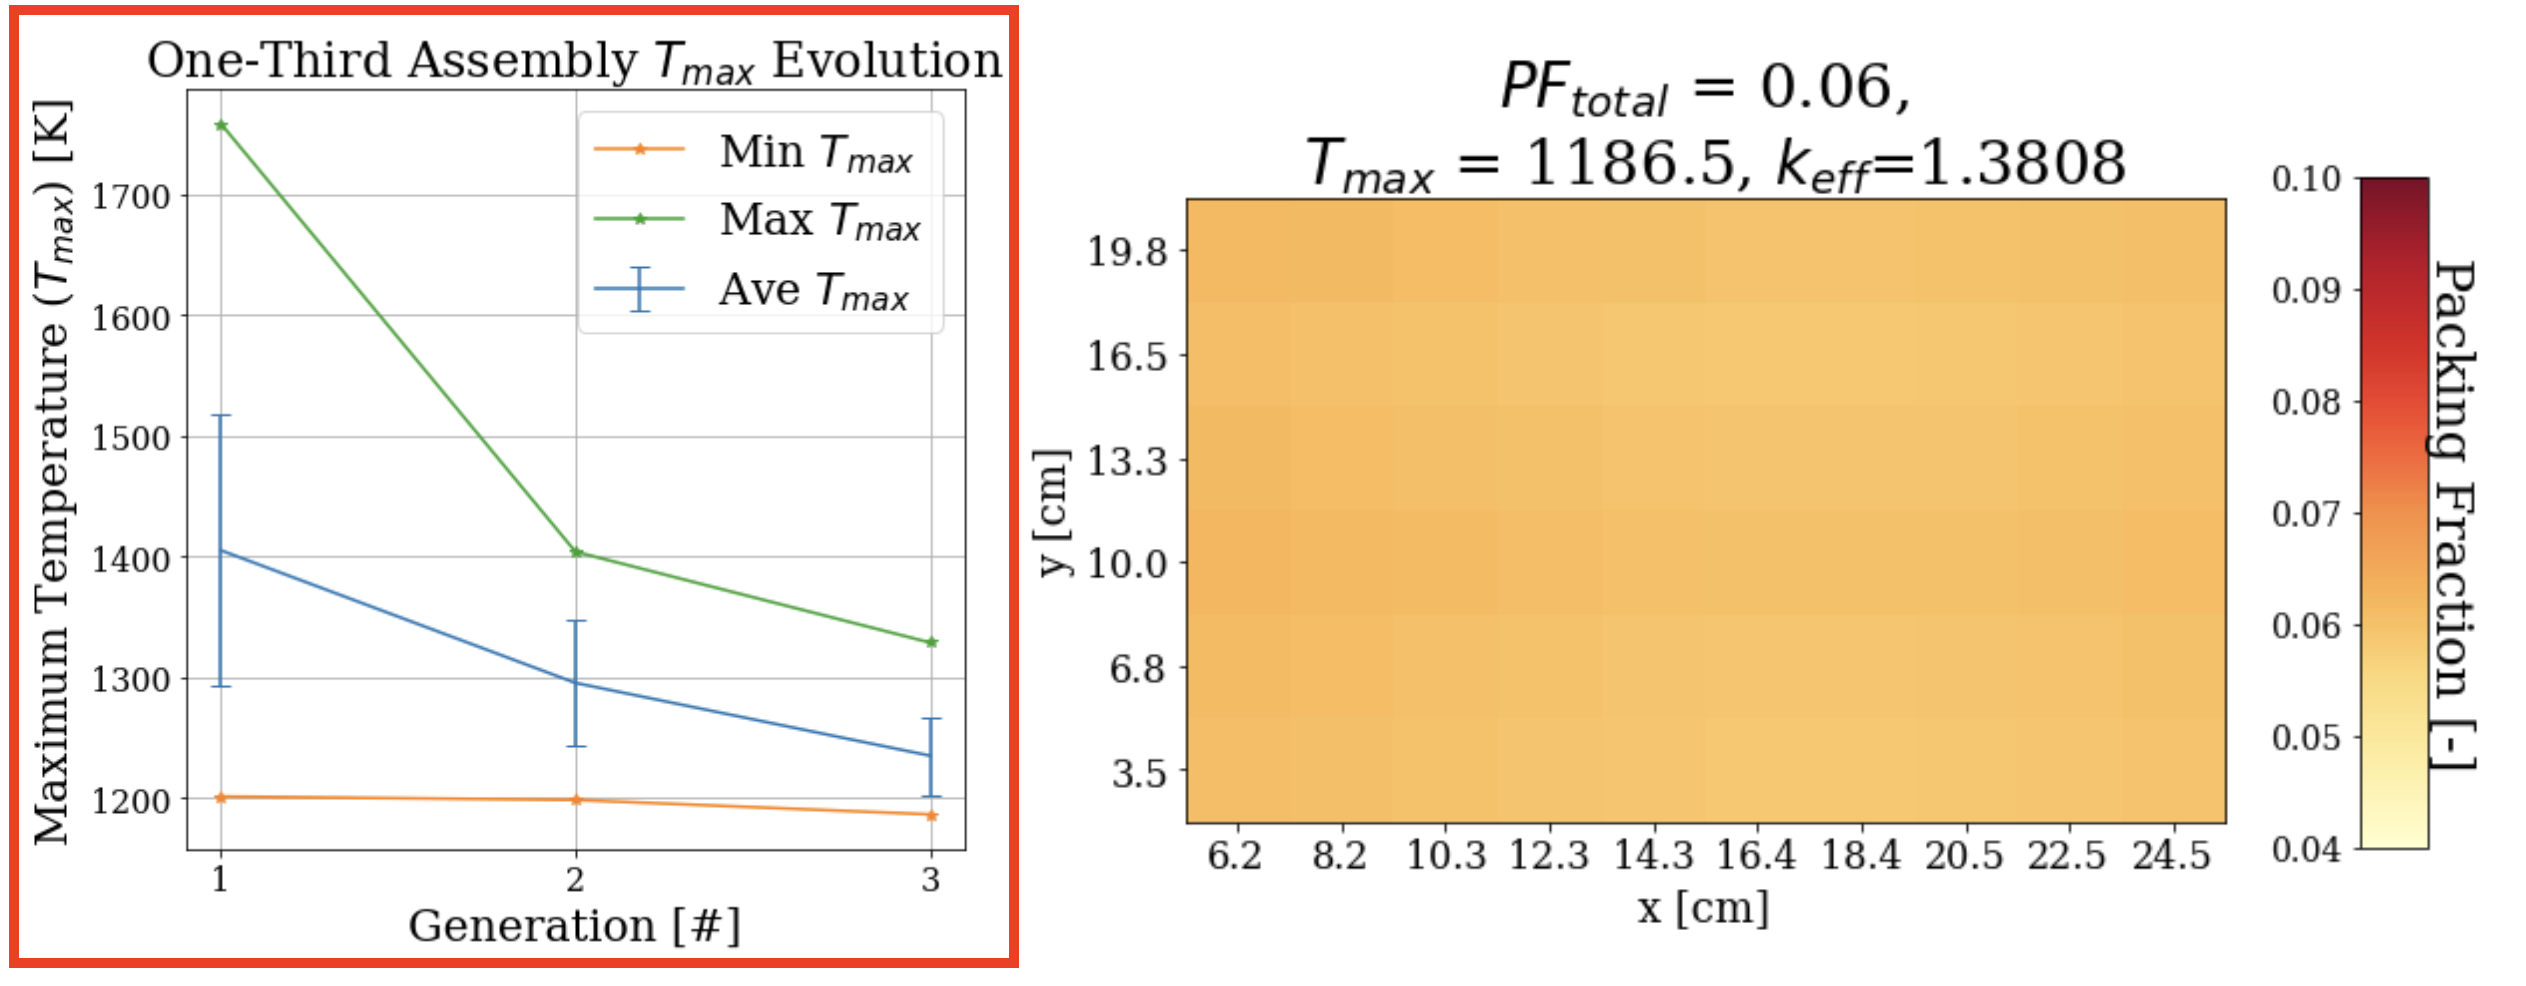
\includegraphics[width=\linewidth]{figures/assem-obj-1-temp-annotated1.png}}
        \only<3>{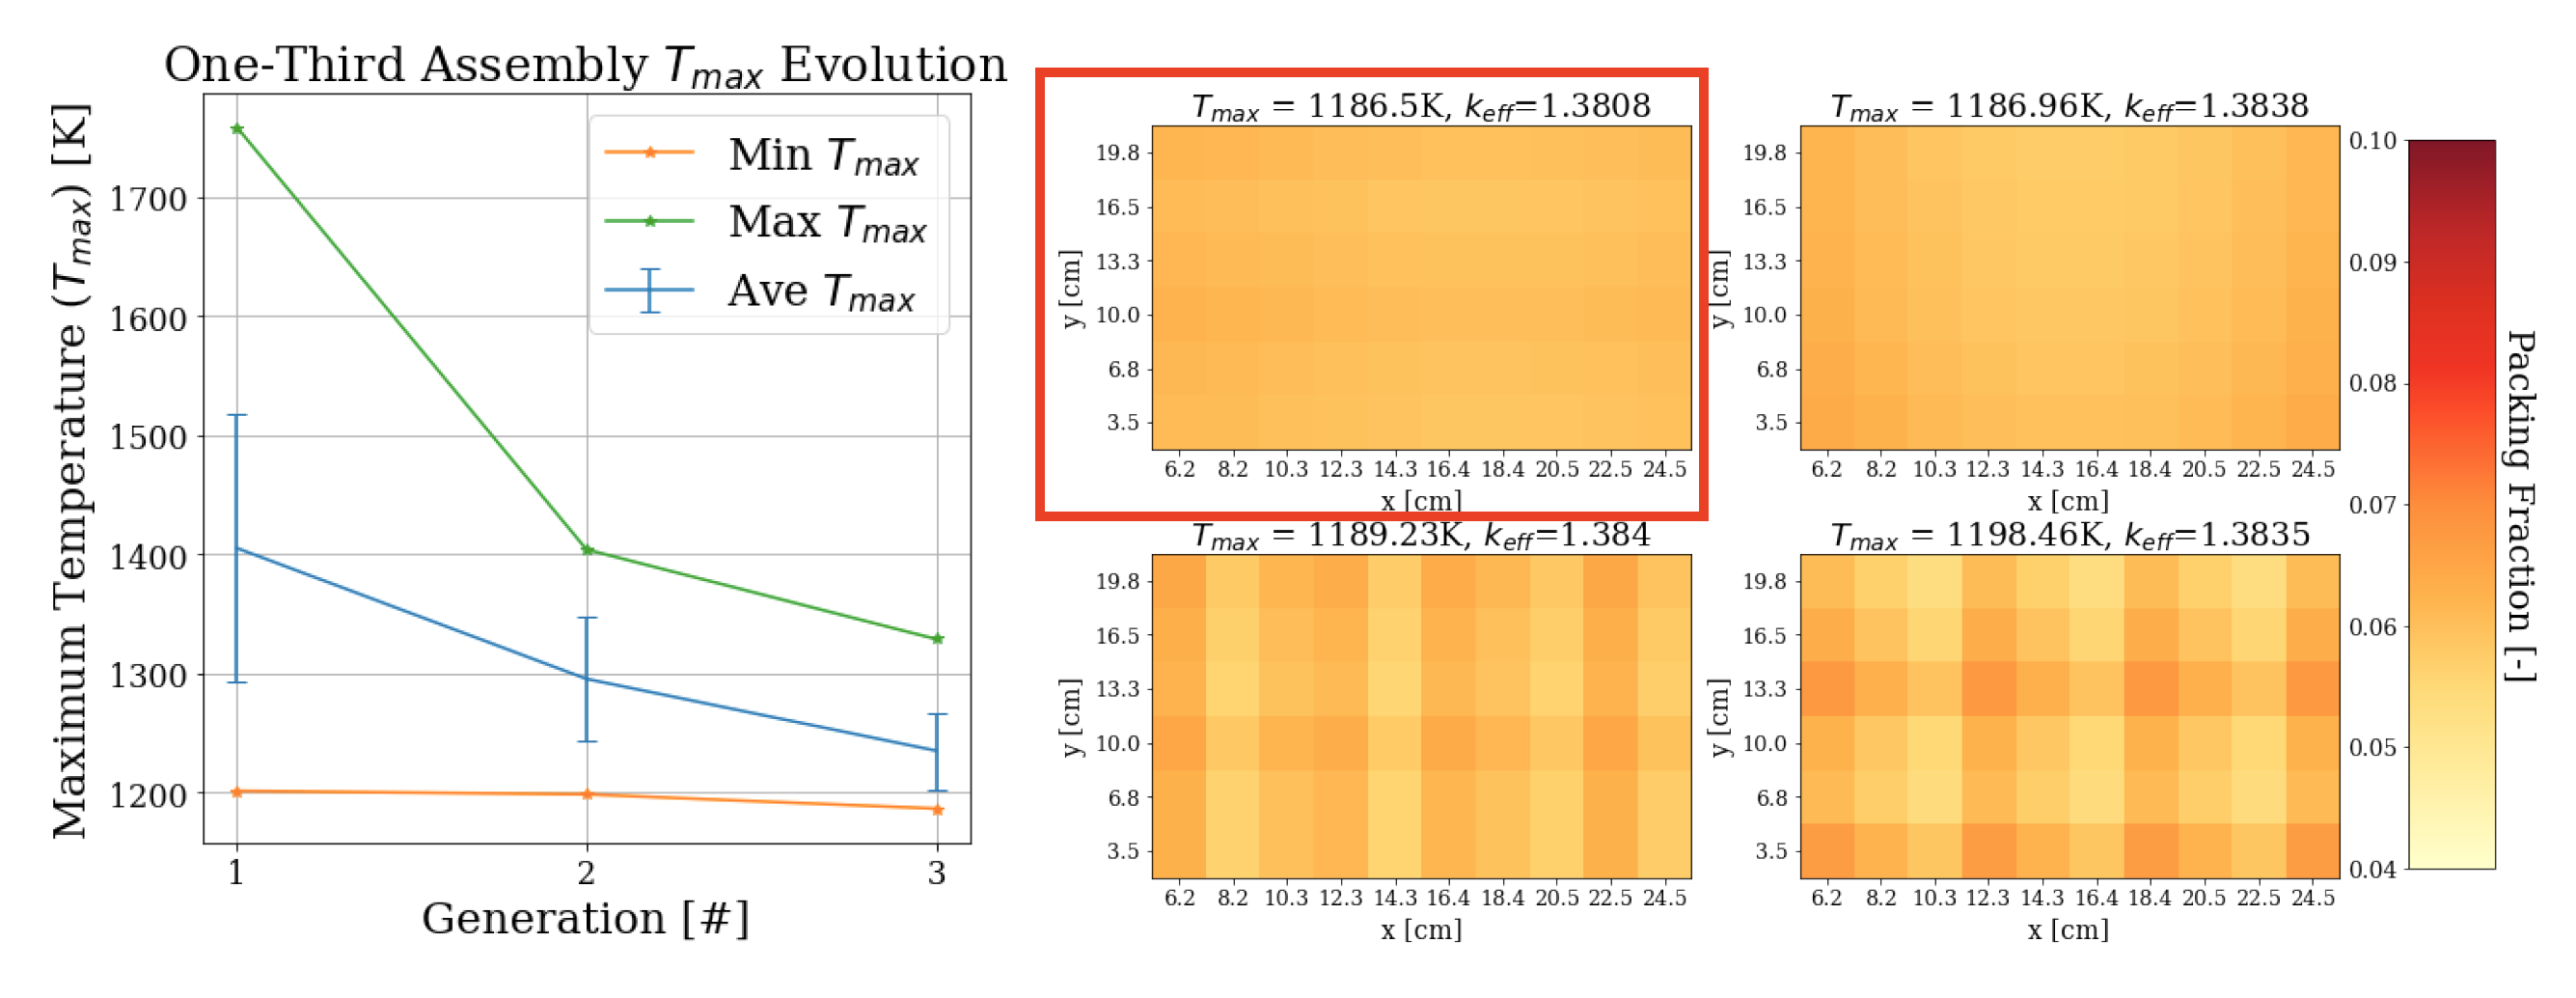
\includegraphics[width=\linewidth]{figures/assem-obj-1-temp-annotated2.png}}
        \vspace{-0.3cm}
        \caption{Simulation a-1b $T_{max}$ evolution and TRISO distribution with lowest 
        $T_{max}$.}
    \end{figure}

    \only<2>{
    \vspace{-0.2cm}
    Simulation a-1b runs for 3 generations with 128 reactor models per 
    generation, the average $T_{max}$ decreased by $\approx$ 100K per generation. 

    \textbf{The average one-third assembly $T_{max}$ converged to $\approx$ 1220K}.}

    \only<3>{\textbf{The TRISO distribution in the final generation with the 
    lowest $T_{max}$ has $T_{max}$ = 1186K and an almost constant TRISO packing fraction 
    distribution.}}

    \only<4>{
    \vspace{-0.4cm}    
    \begin{tcolorbox}[colback=illiniorange,colframe=illiniorange!50!black]
        \textbf{A flatter TRISO distribution minimizes $T_{max}$.}
    \end{tcolorbox}}
\end{frame}

\begin{frame}
    \frametitle{AHTR One-Third Assembly Simulation a-1e Results}
    \visible<1->{\textbf{I vary $r_1, r_2, r_3, r_4, r_5$ (coolant channel shape)
    to minimize $T_{max}$.}}

    \begin{figure}
        \centering
        \begin{subfigure}{0.3\textwidth}
            \only<1,3>{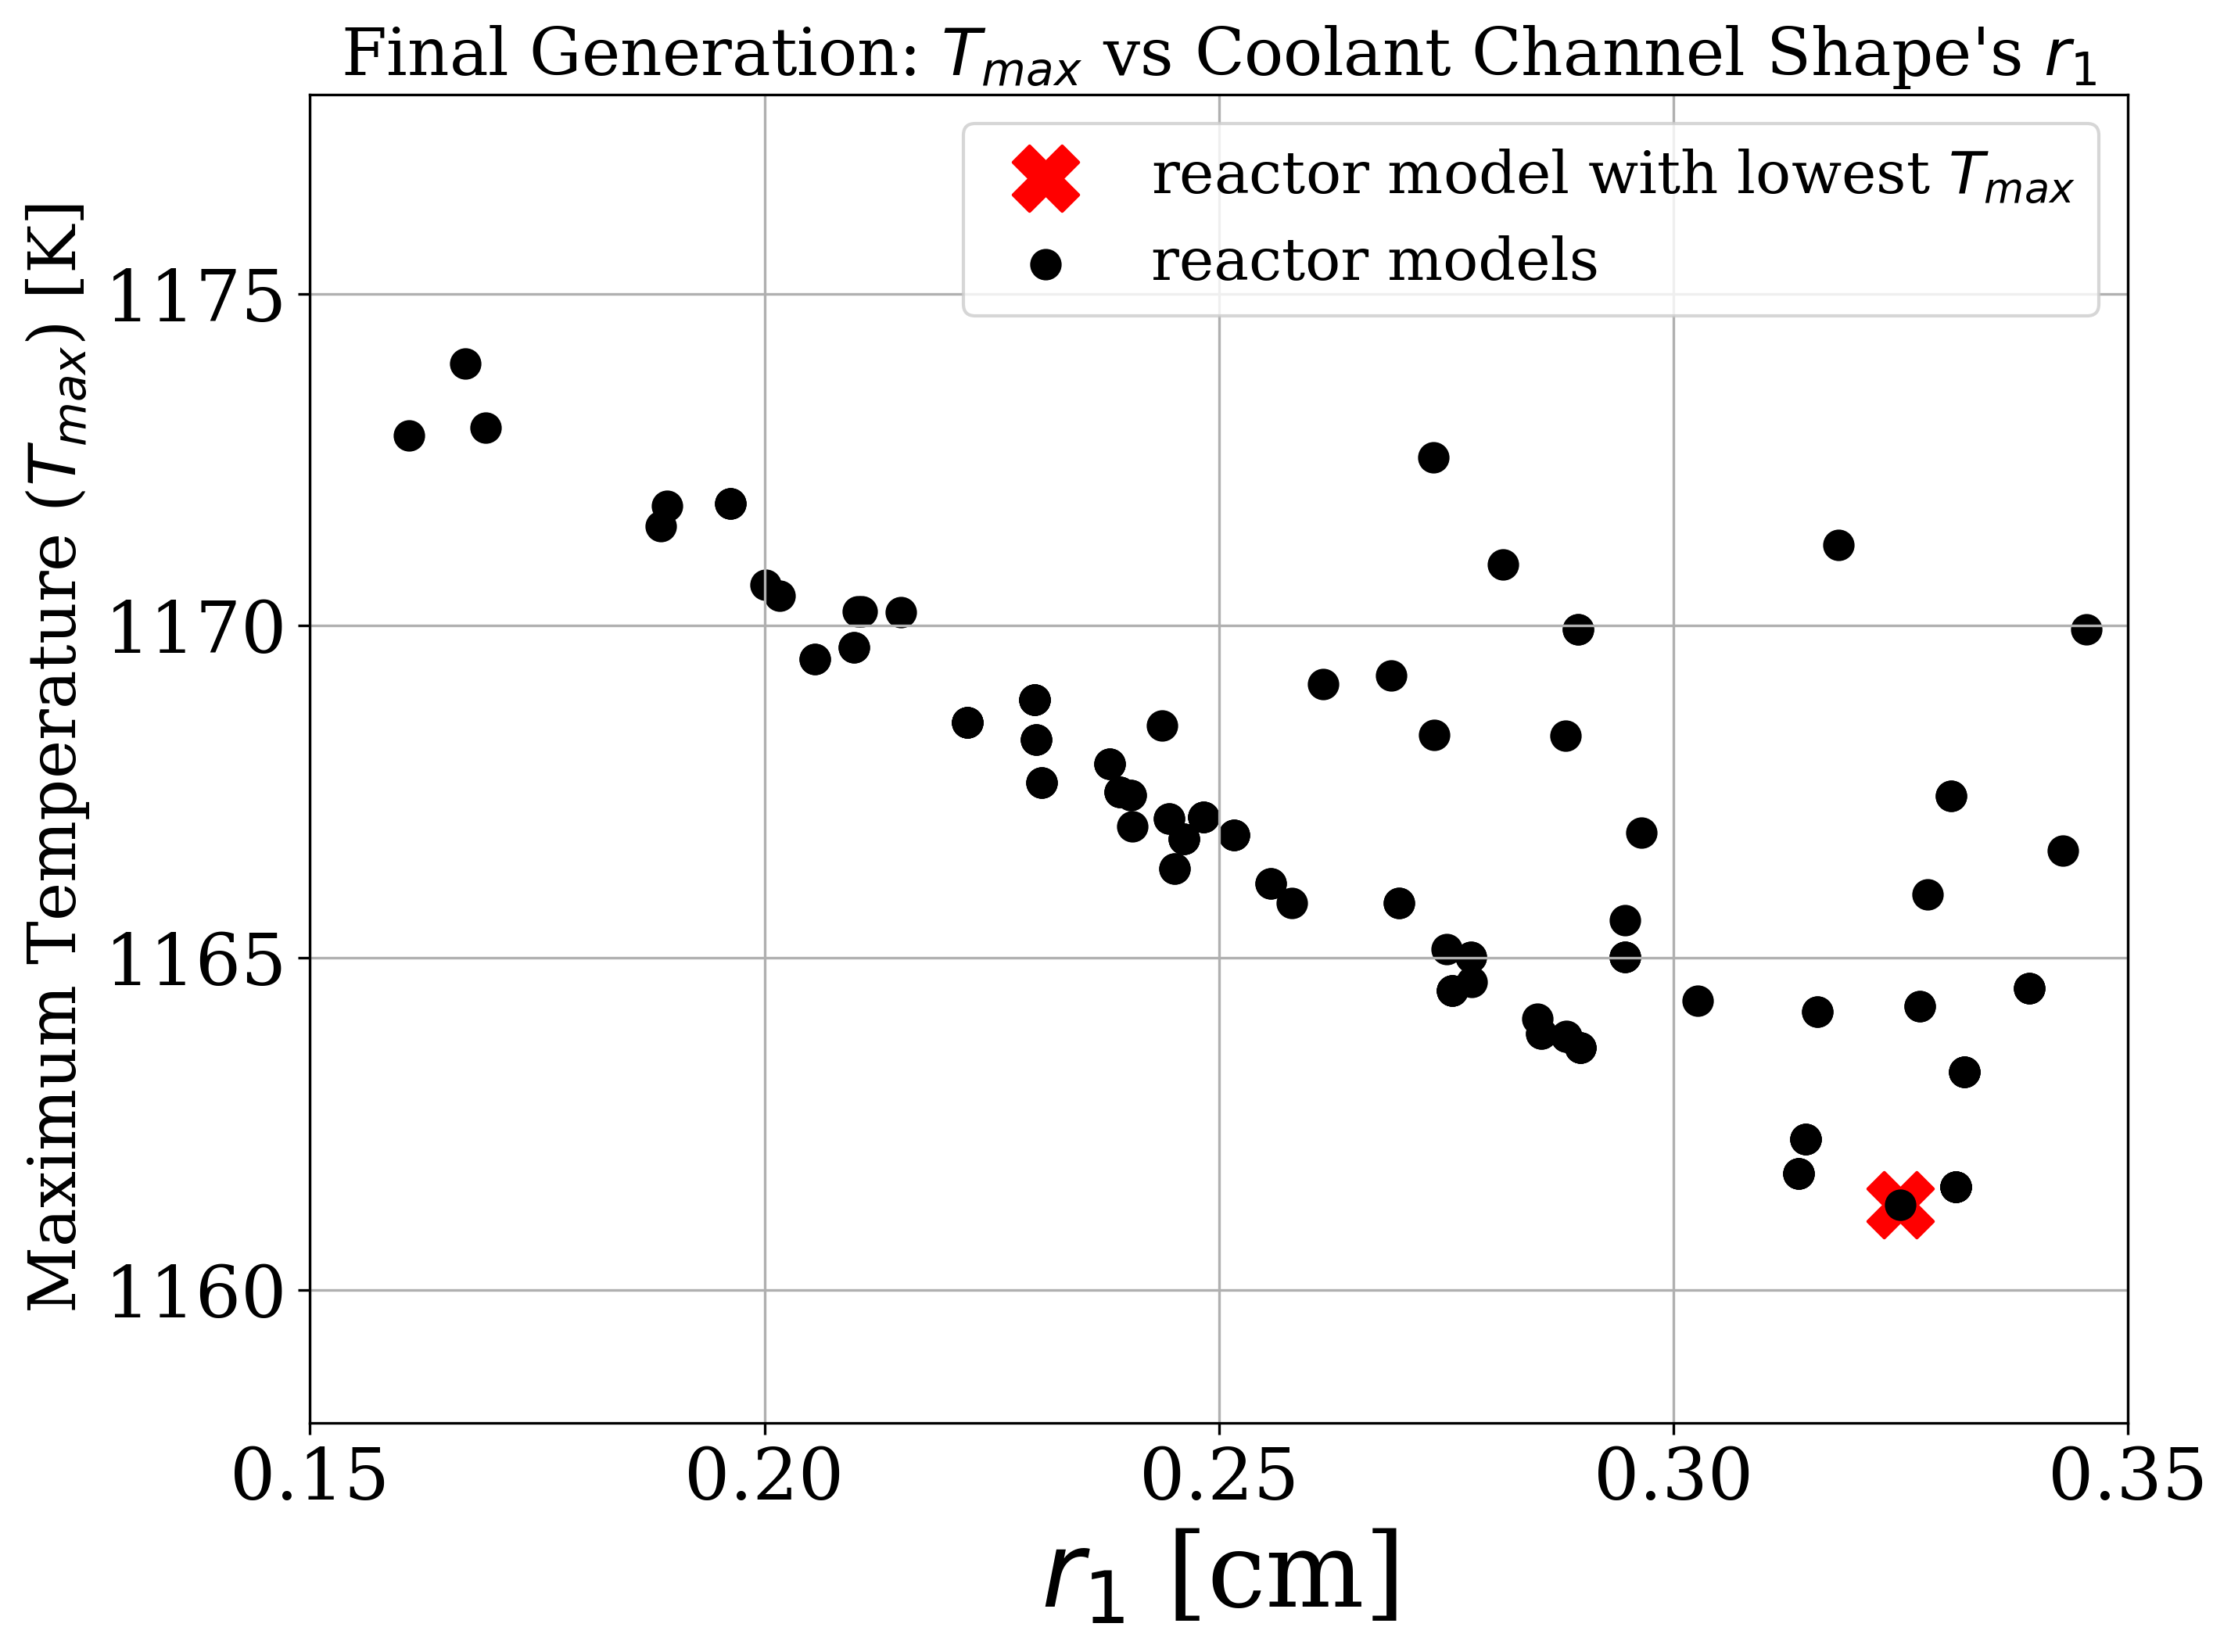
\includegraphics[width=\linewidth]{figures/a-1e-r1-pres.png}}
            \only<2>{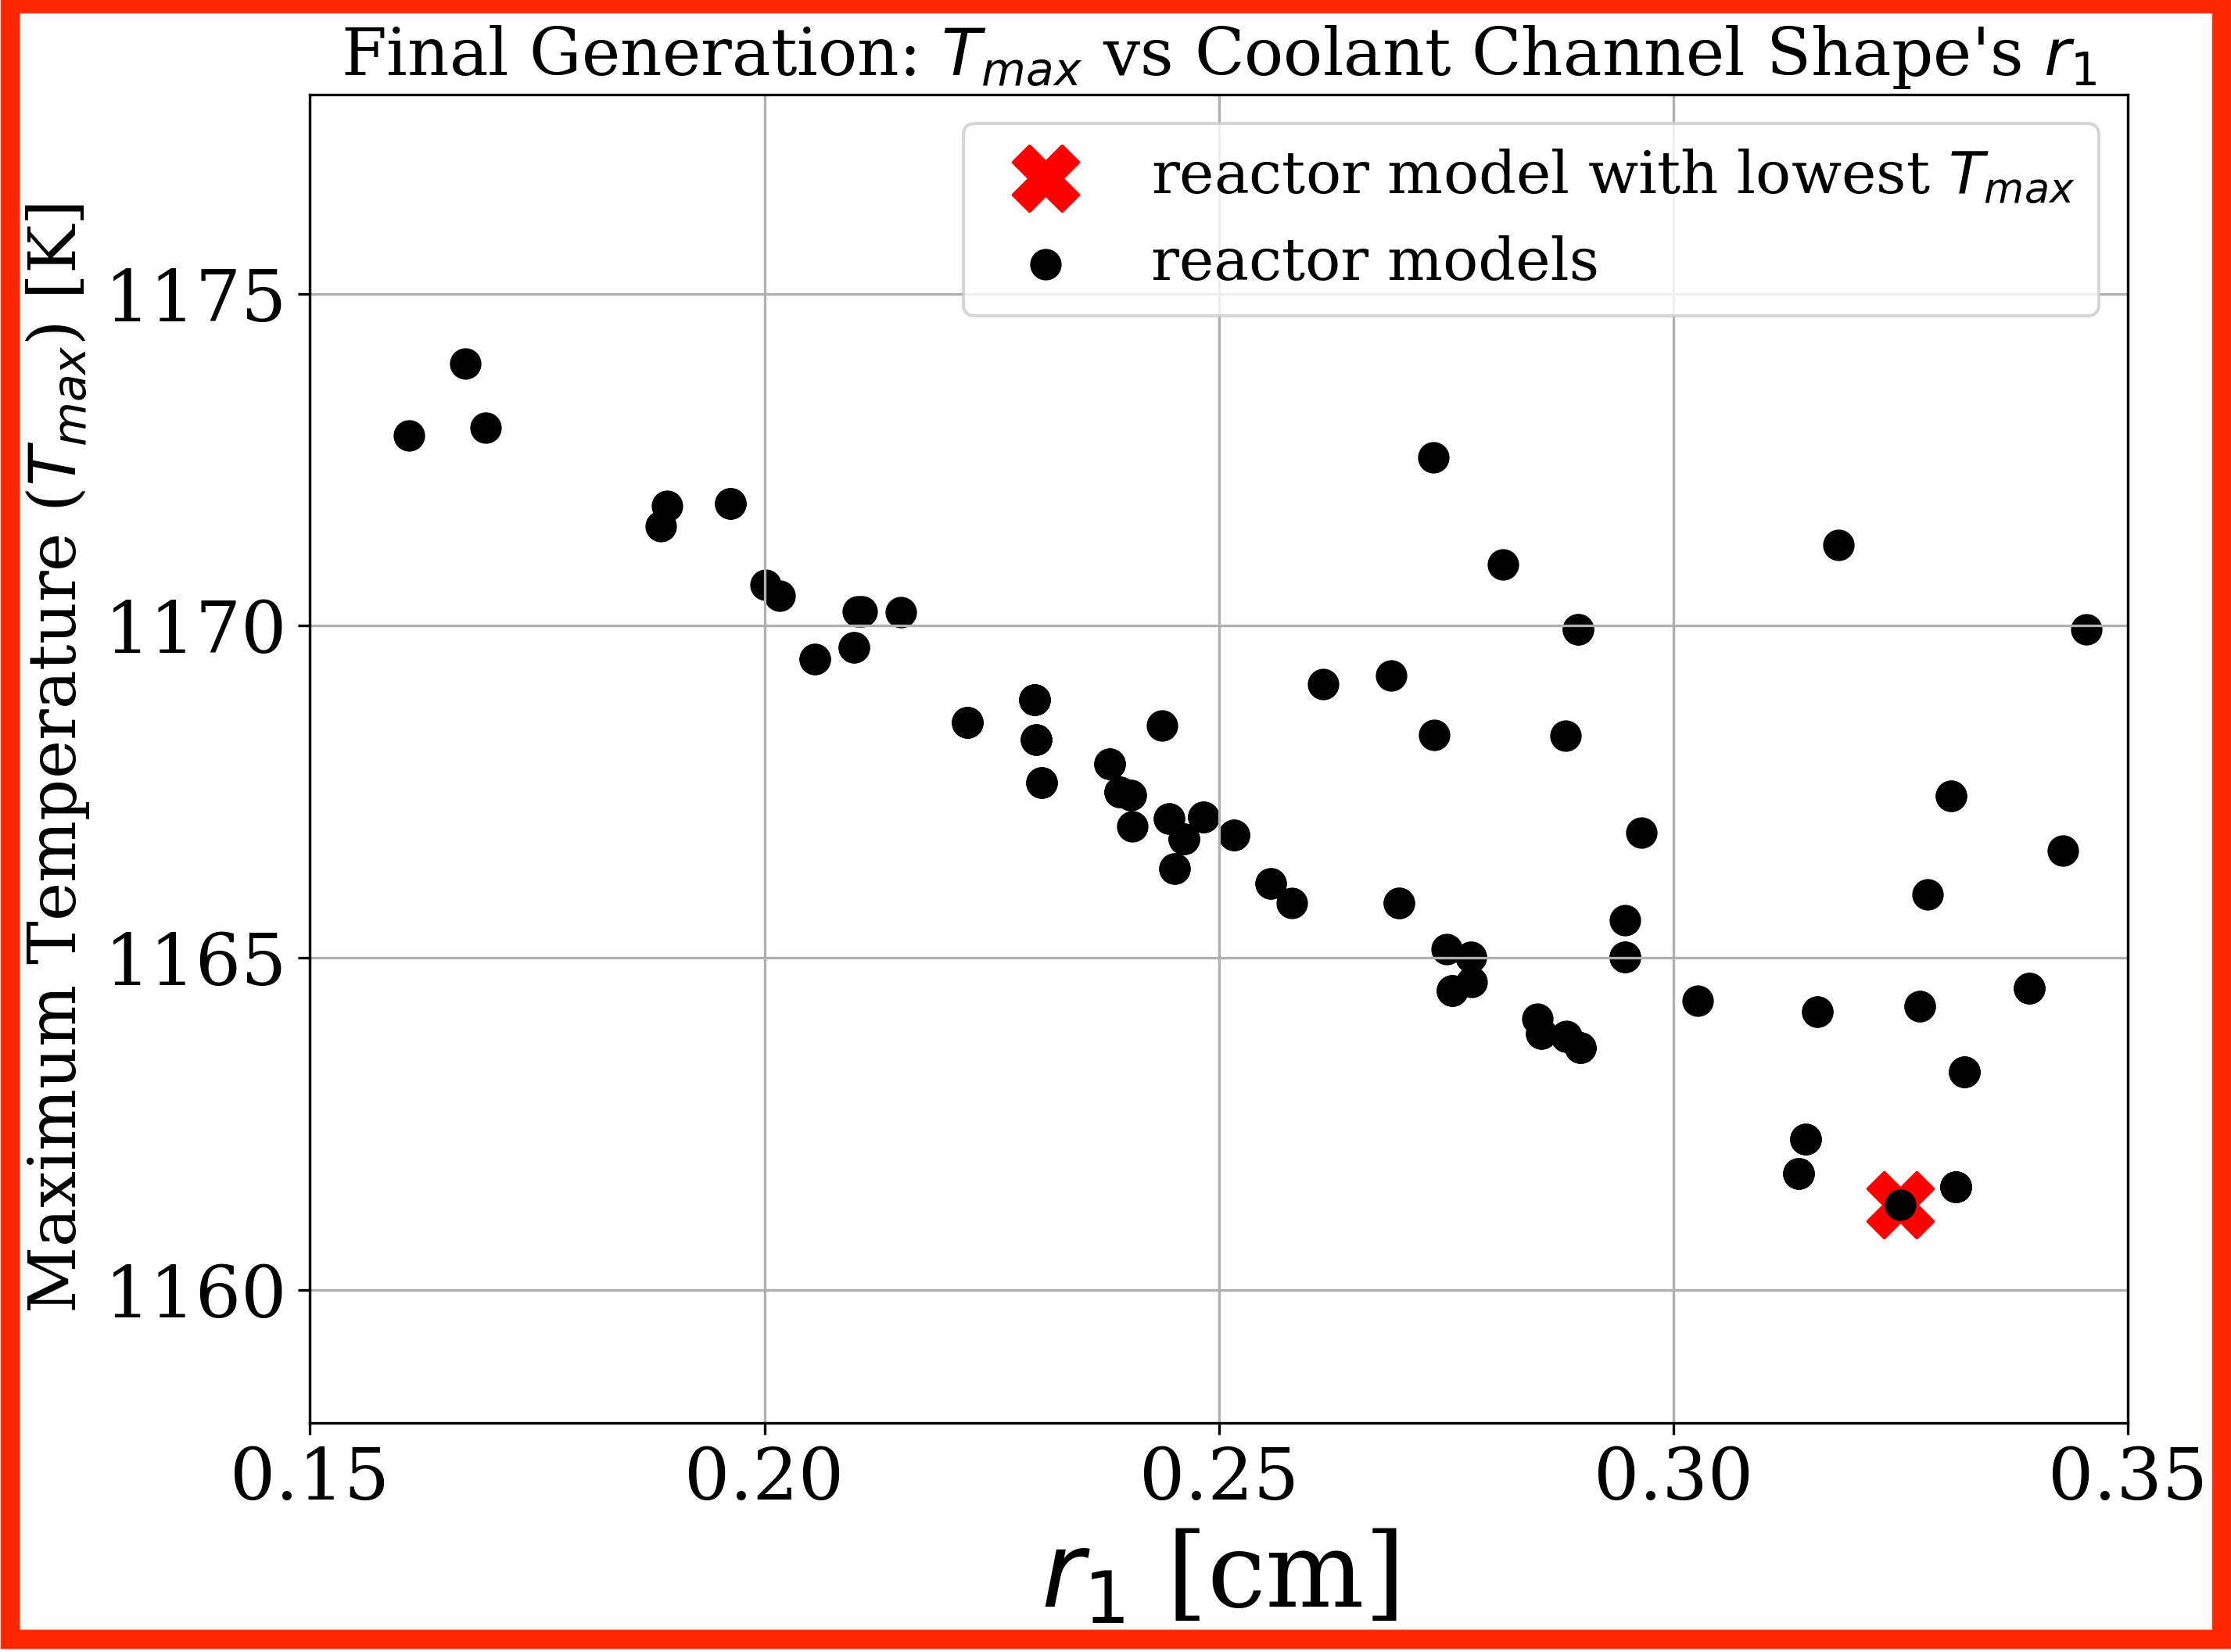
\includegraphics[width=\linewidth]{figures/a-1e-r1-pres-annotated.png}}
            \vspace{-0.5cm}
            \caption{Plot of $T_{max}$ against $r_1$.}
        \end{subfigure}
        \begin{subfigure}{0.3\textwidth}
            \only<1,2>{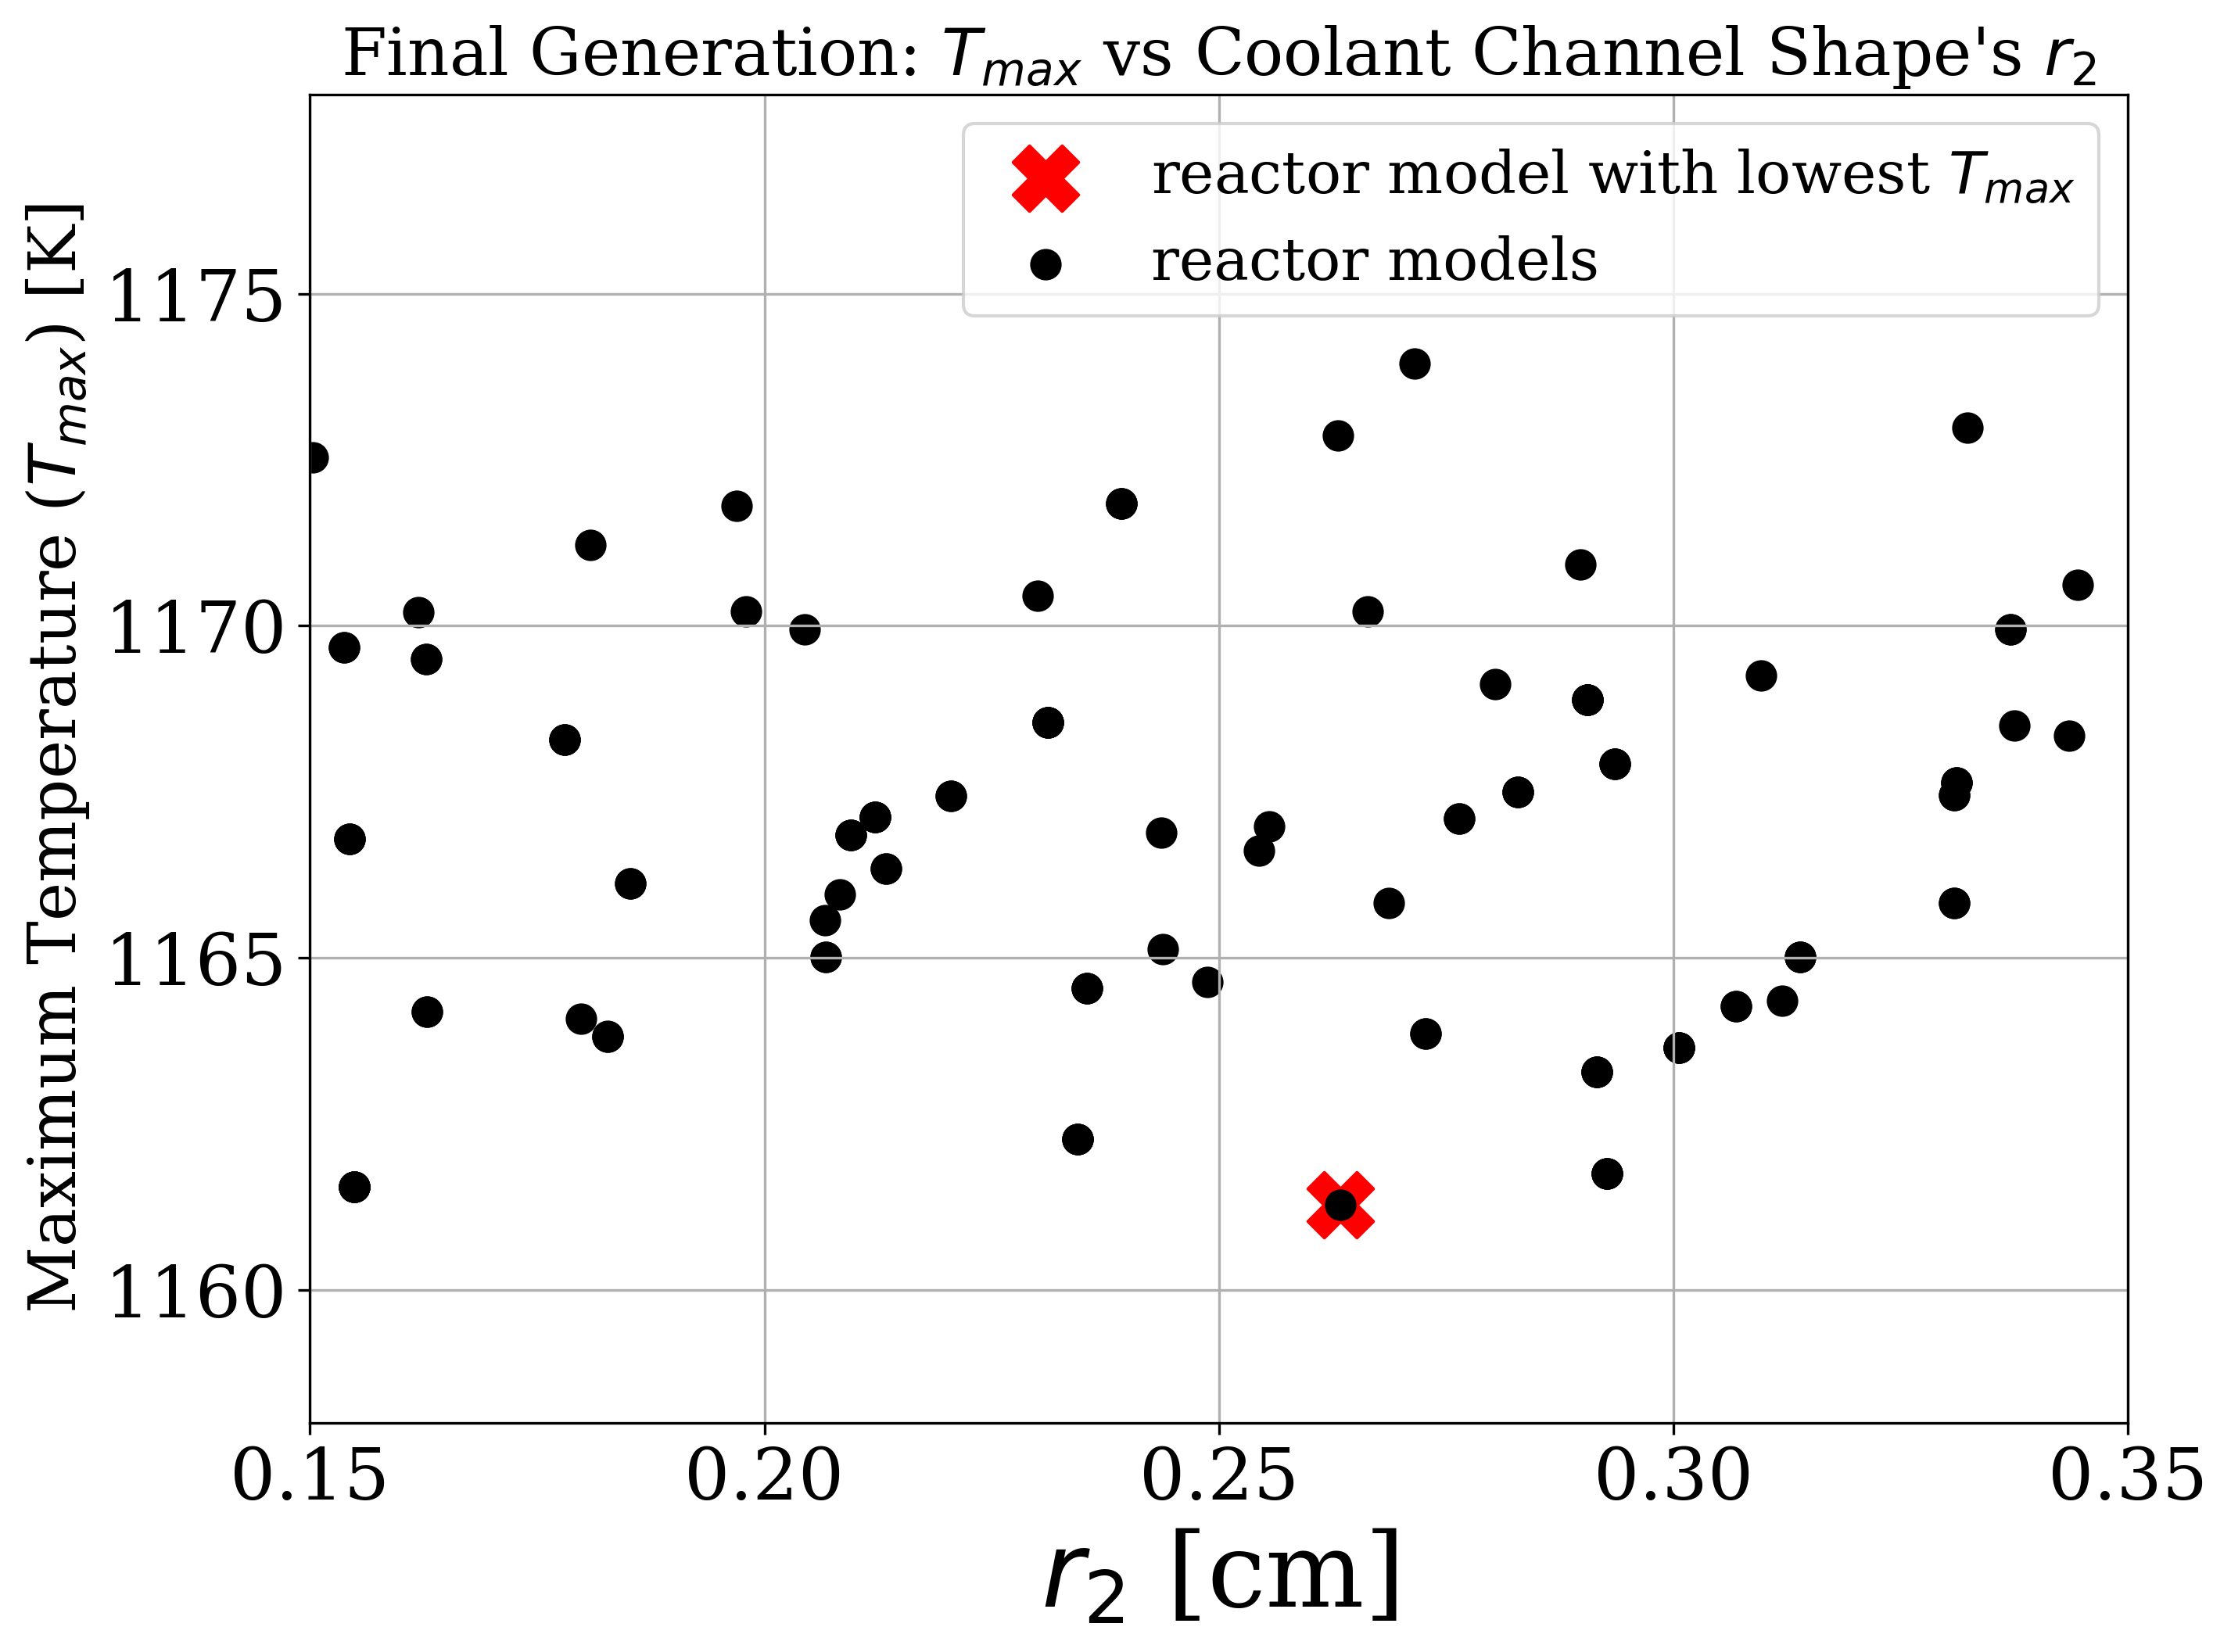
\includegraphics[width=\linewidth]{figures/a-1e-r2-pres.png}}
            \only<3>{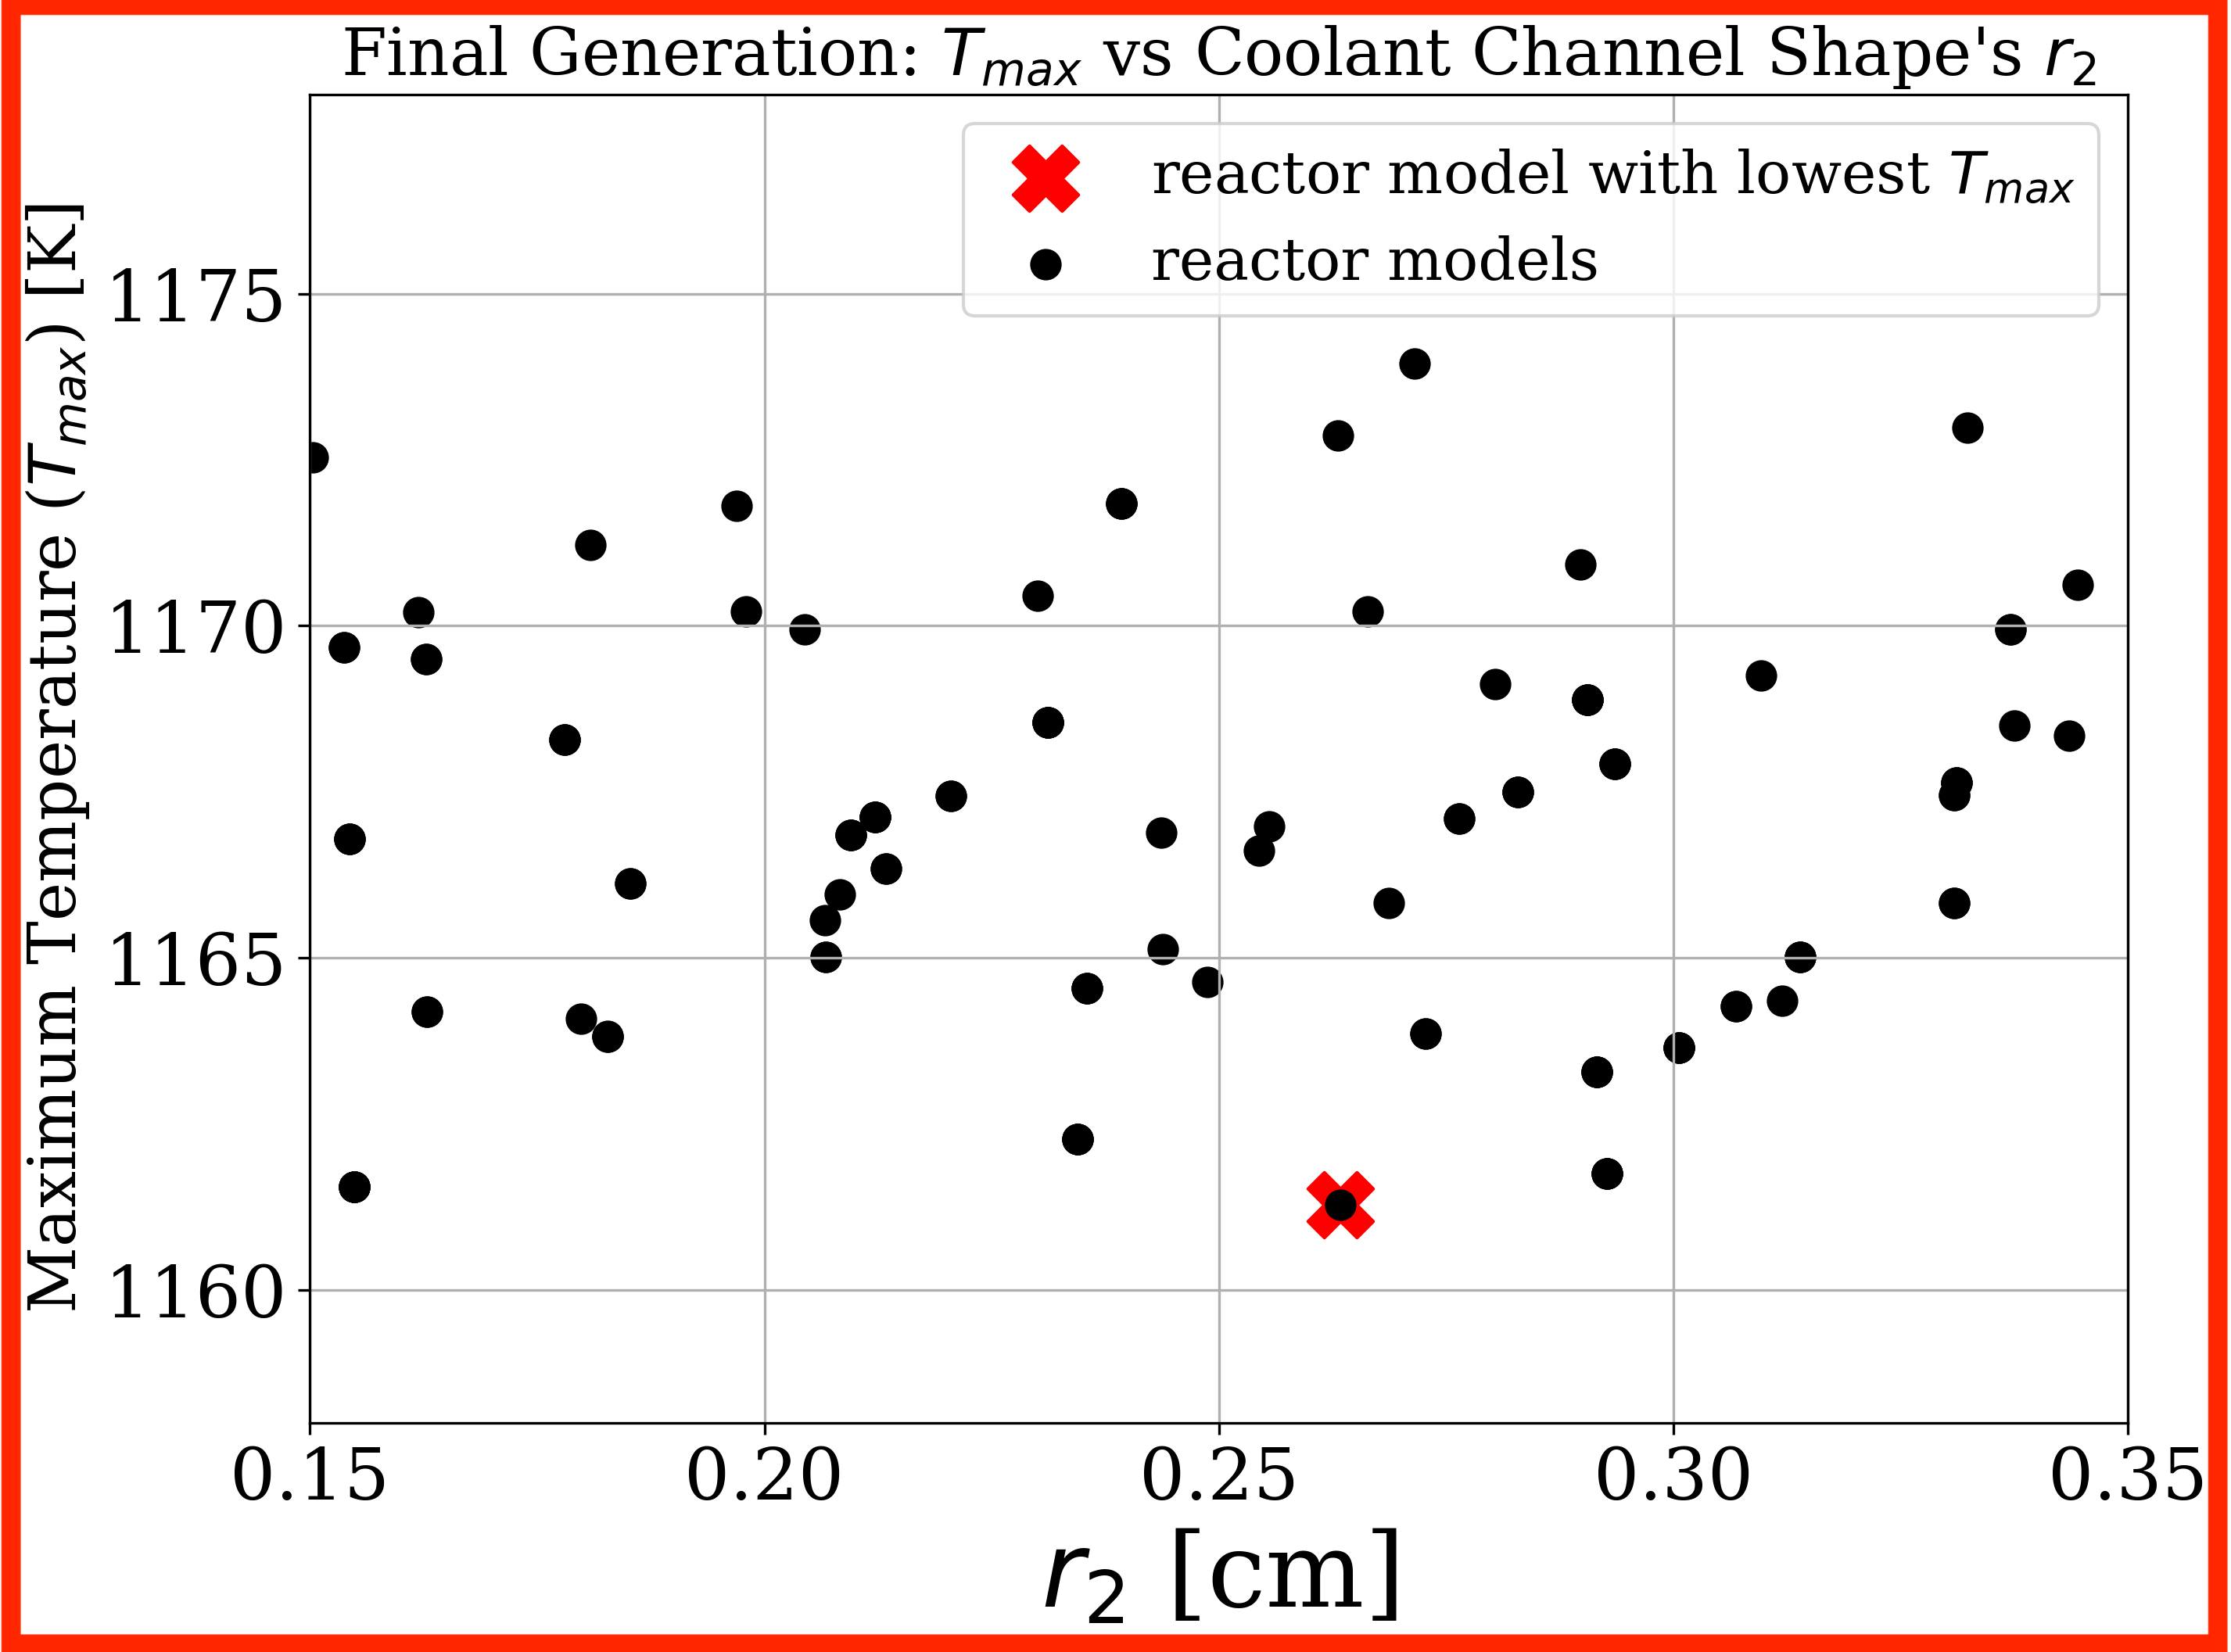
\includegraphics[width=\linewidth]{figures/a-1e-r2-pres-annotated.png}}
            \vspace{-0.5cm}
            \caption{Plot of $T_{max}$ against $r_2$.}
        \end{subfigure}
        \begin{subfigure}{0.3\textwidth}
            \only<1,2>{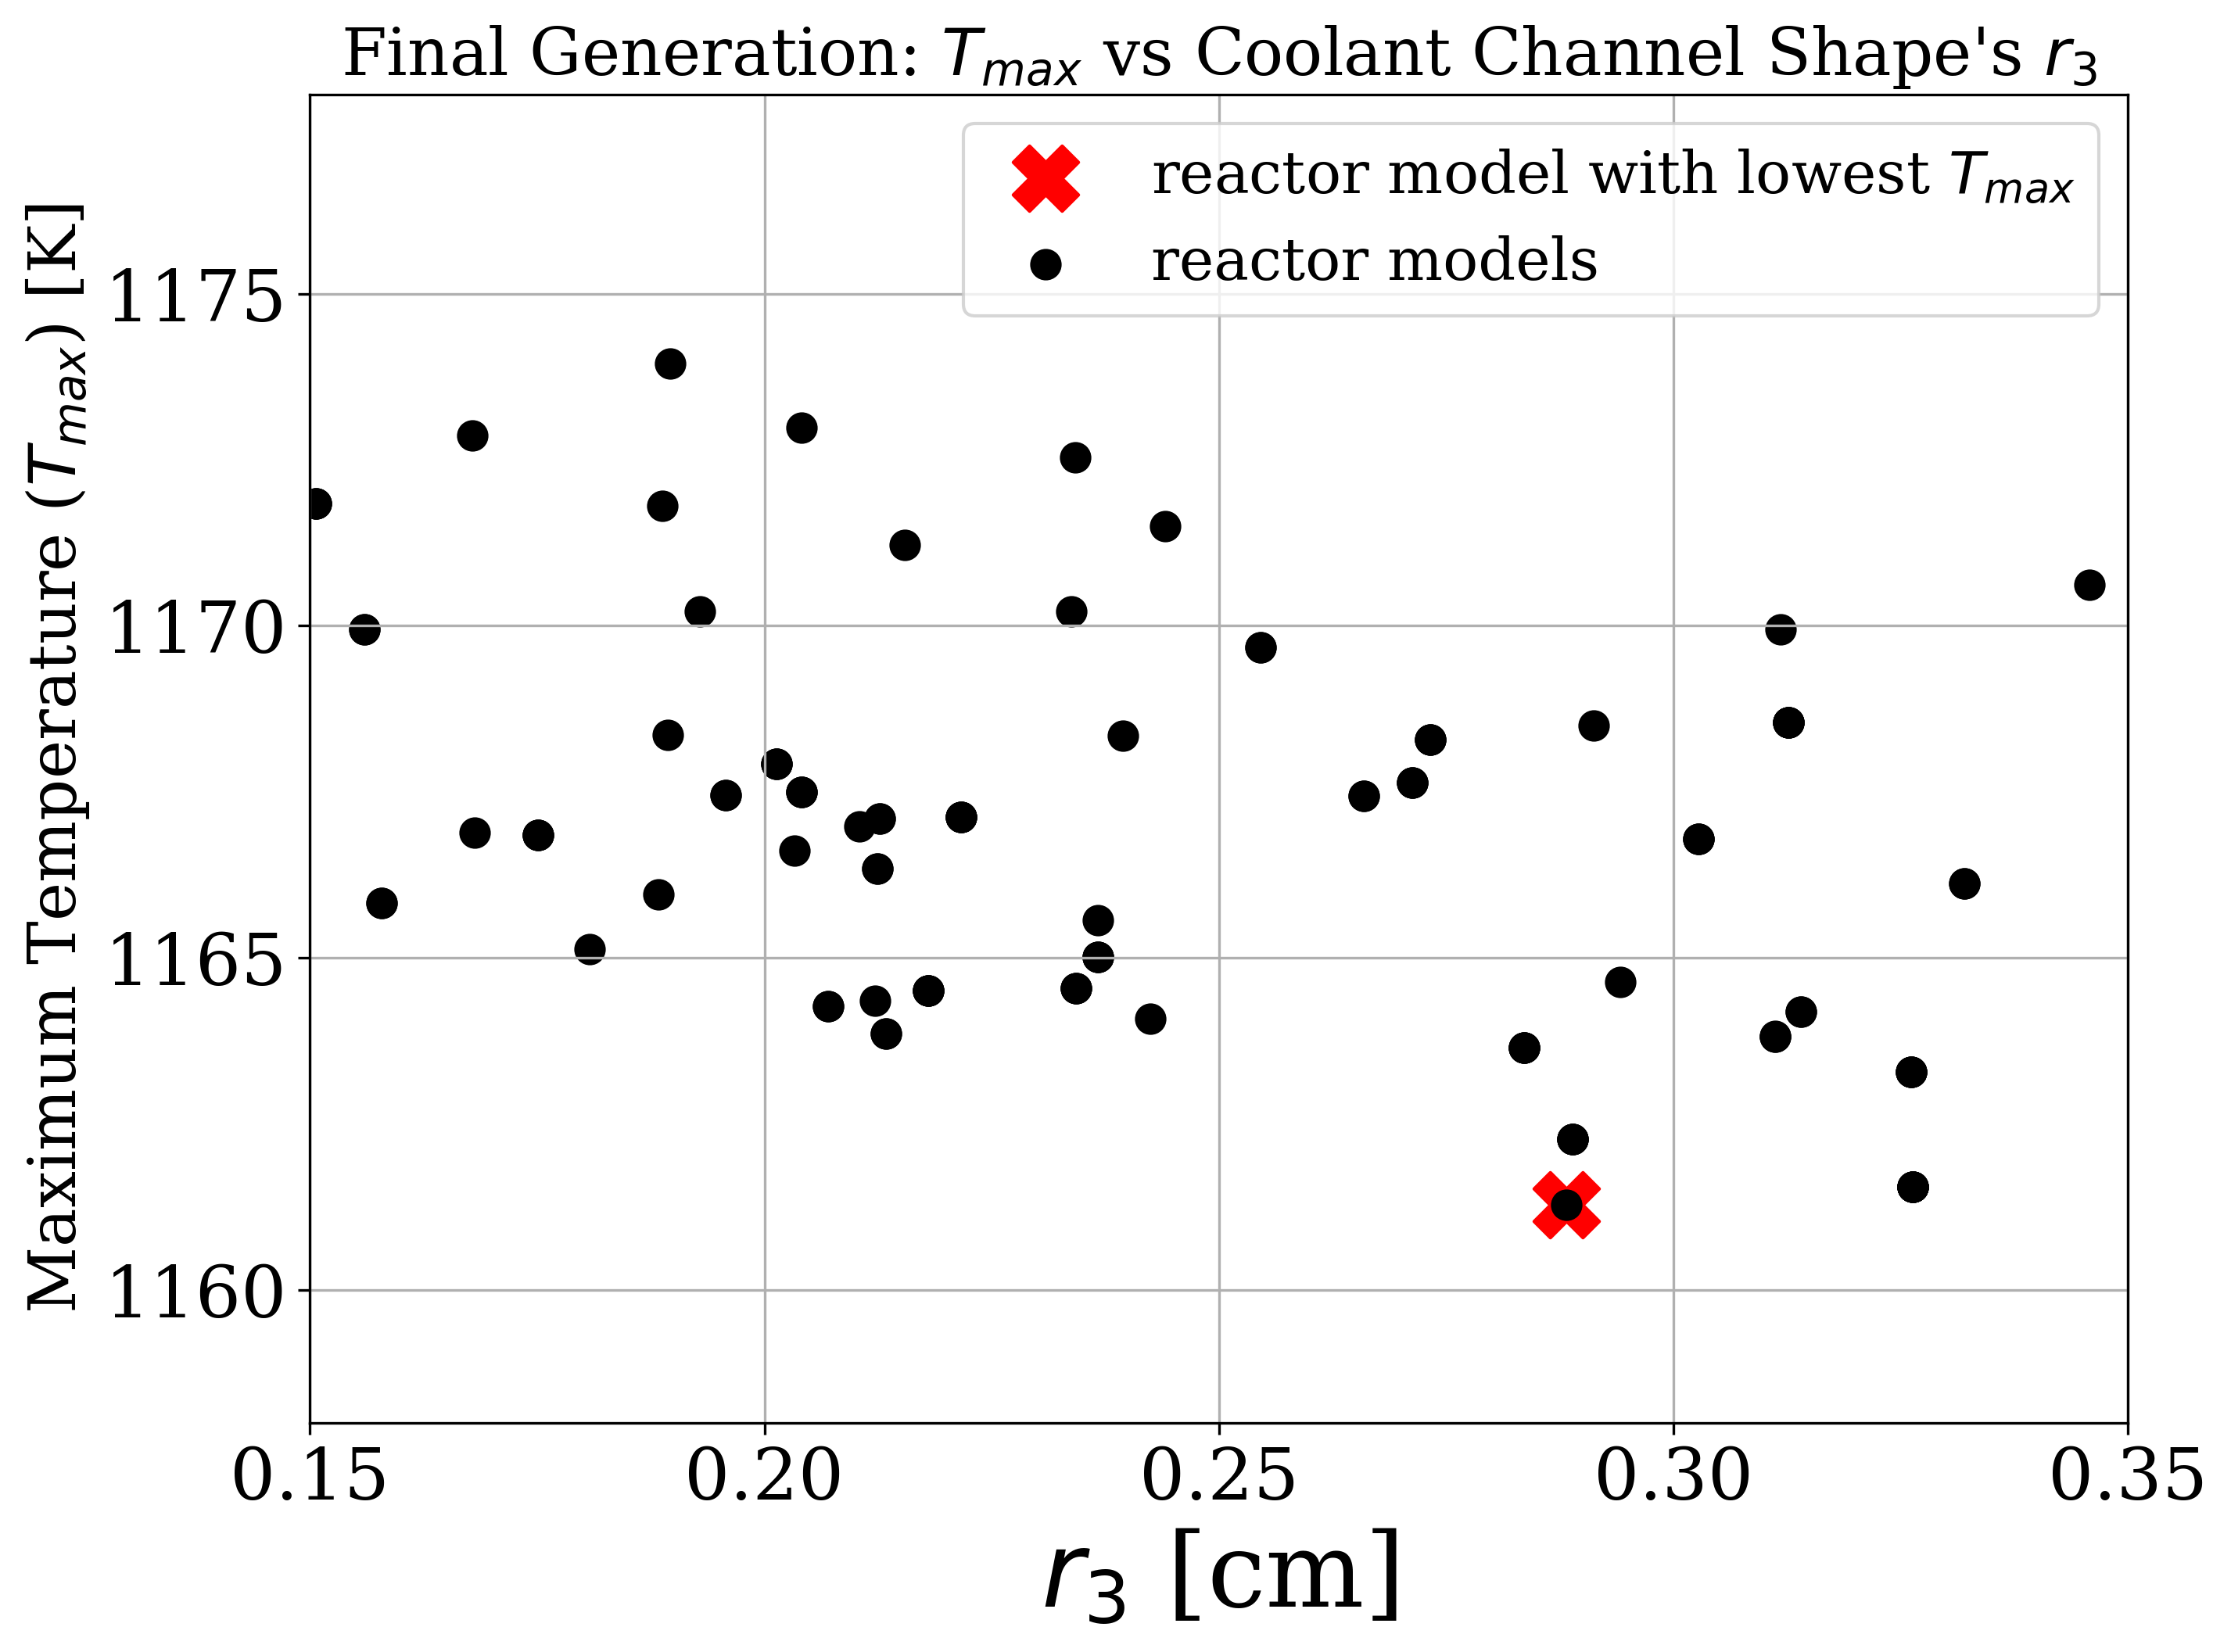
\includegraphics[width=\linewidth]{figures/a-1e-r3-pres.png}}
            \only<3>{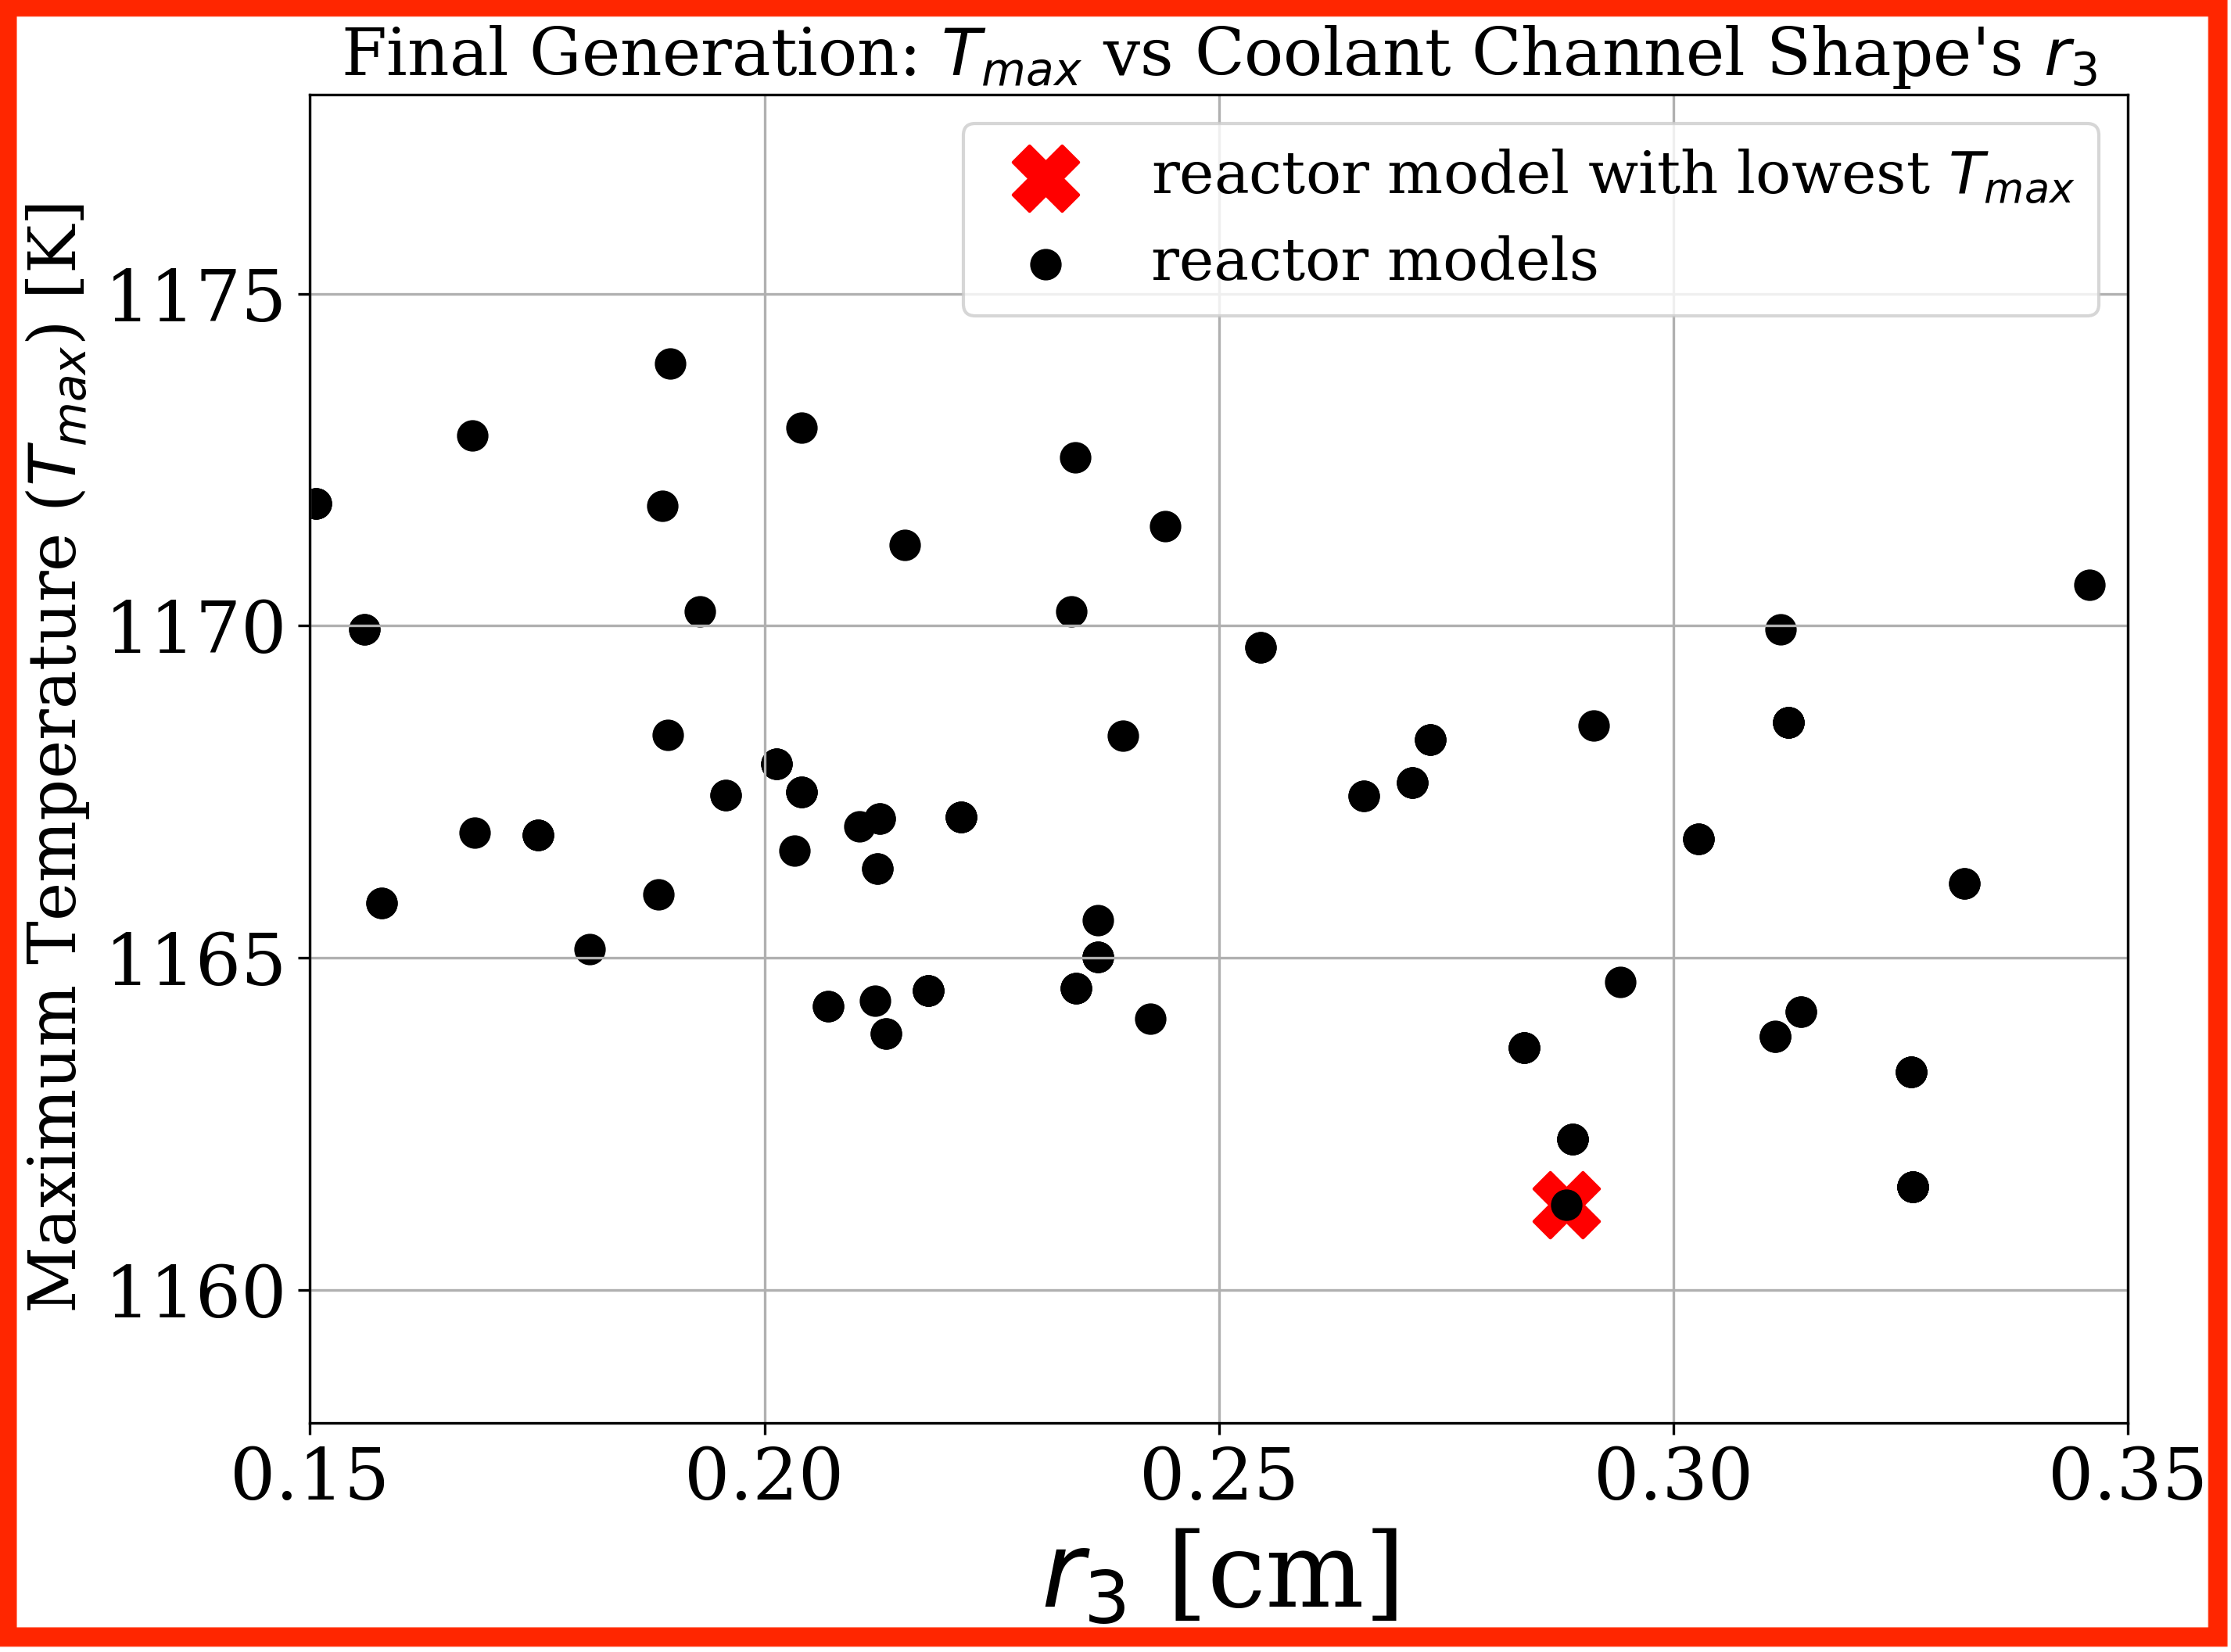
\includegraphics[width=\linewidth]{figures/a-1e-r3-pres-annotated.png}}
            \vspace{-0.5cm}
            \caption{Plot of $T_{max}$ against $r_3$.}
        \end{subfigure}
        \begin{subfigure}{0.3\textwidth}
            \only<1,2>{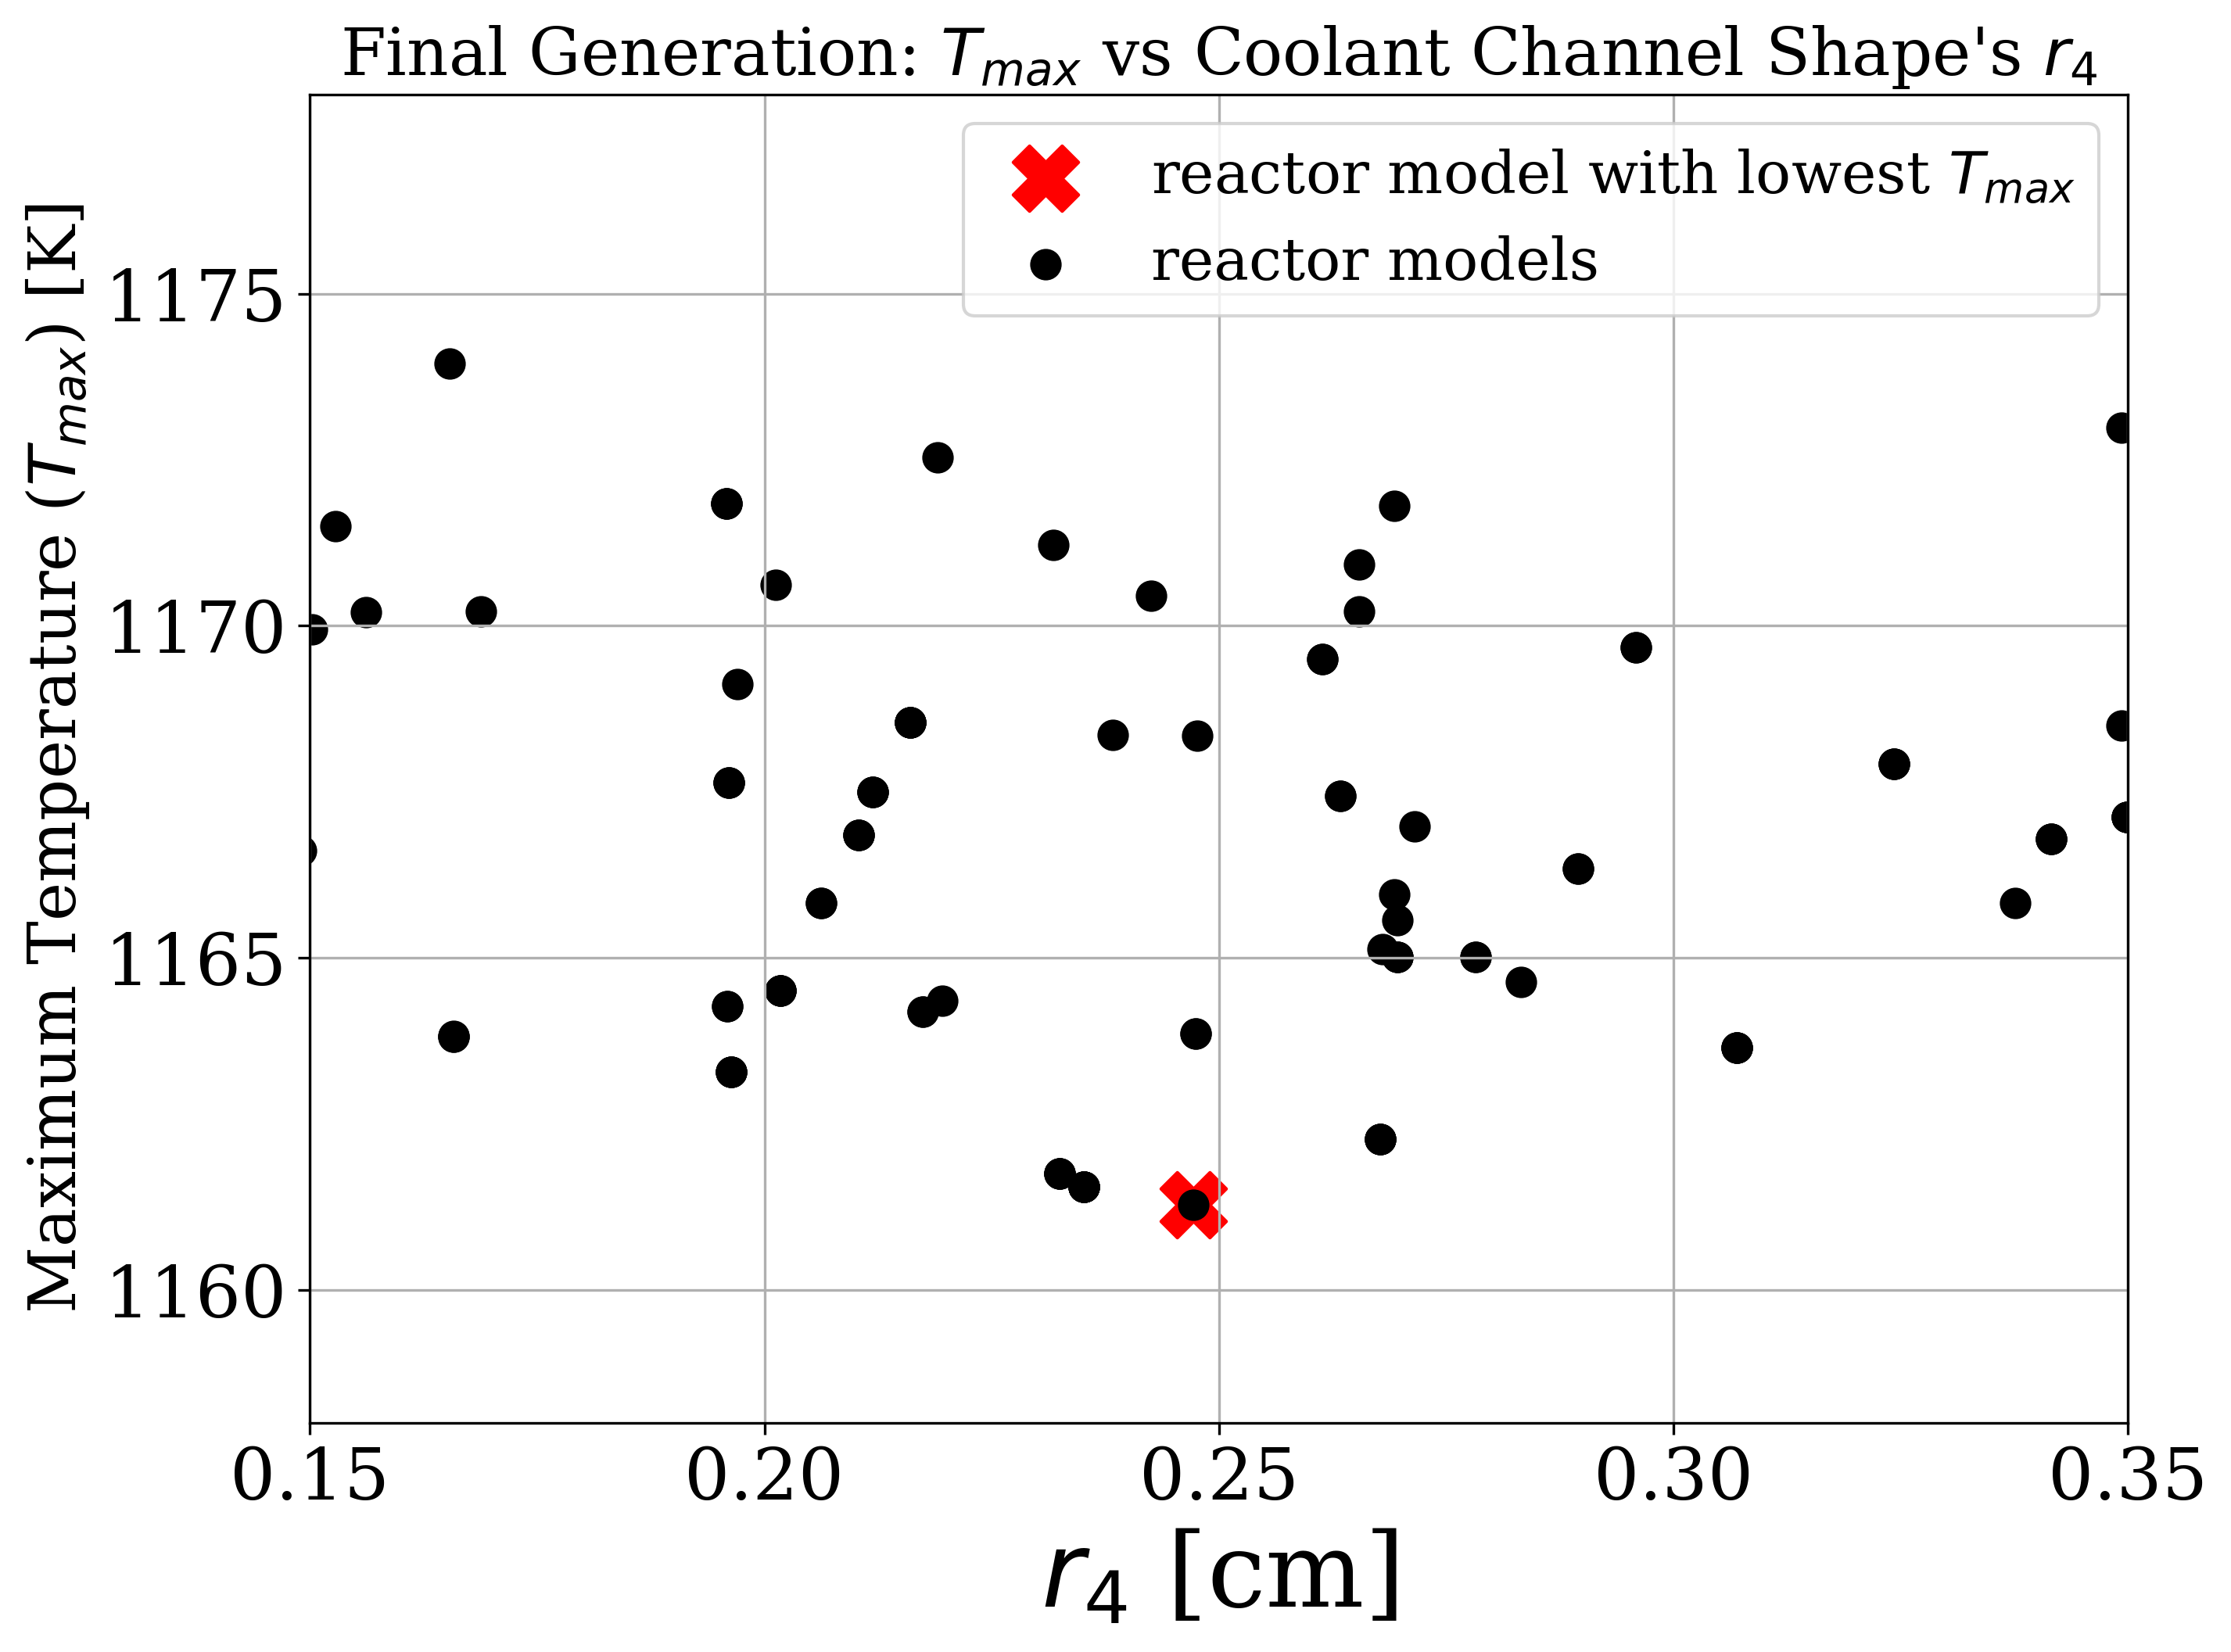
\includegraphics[width=\linewidth]{figures/a-1e-r4-pres.png}}
            \only<3>{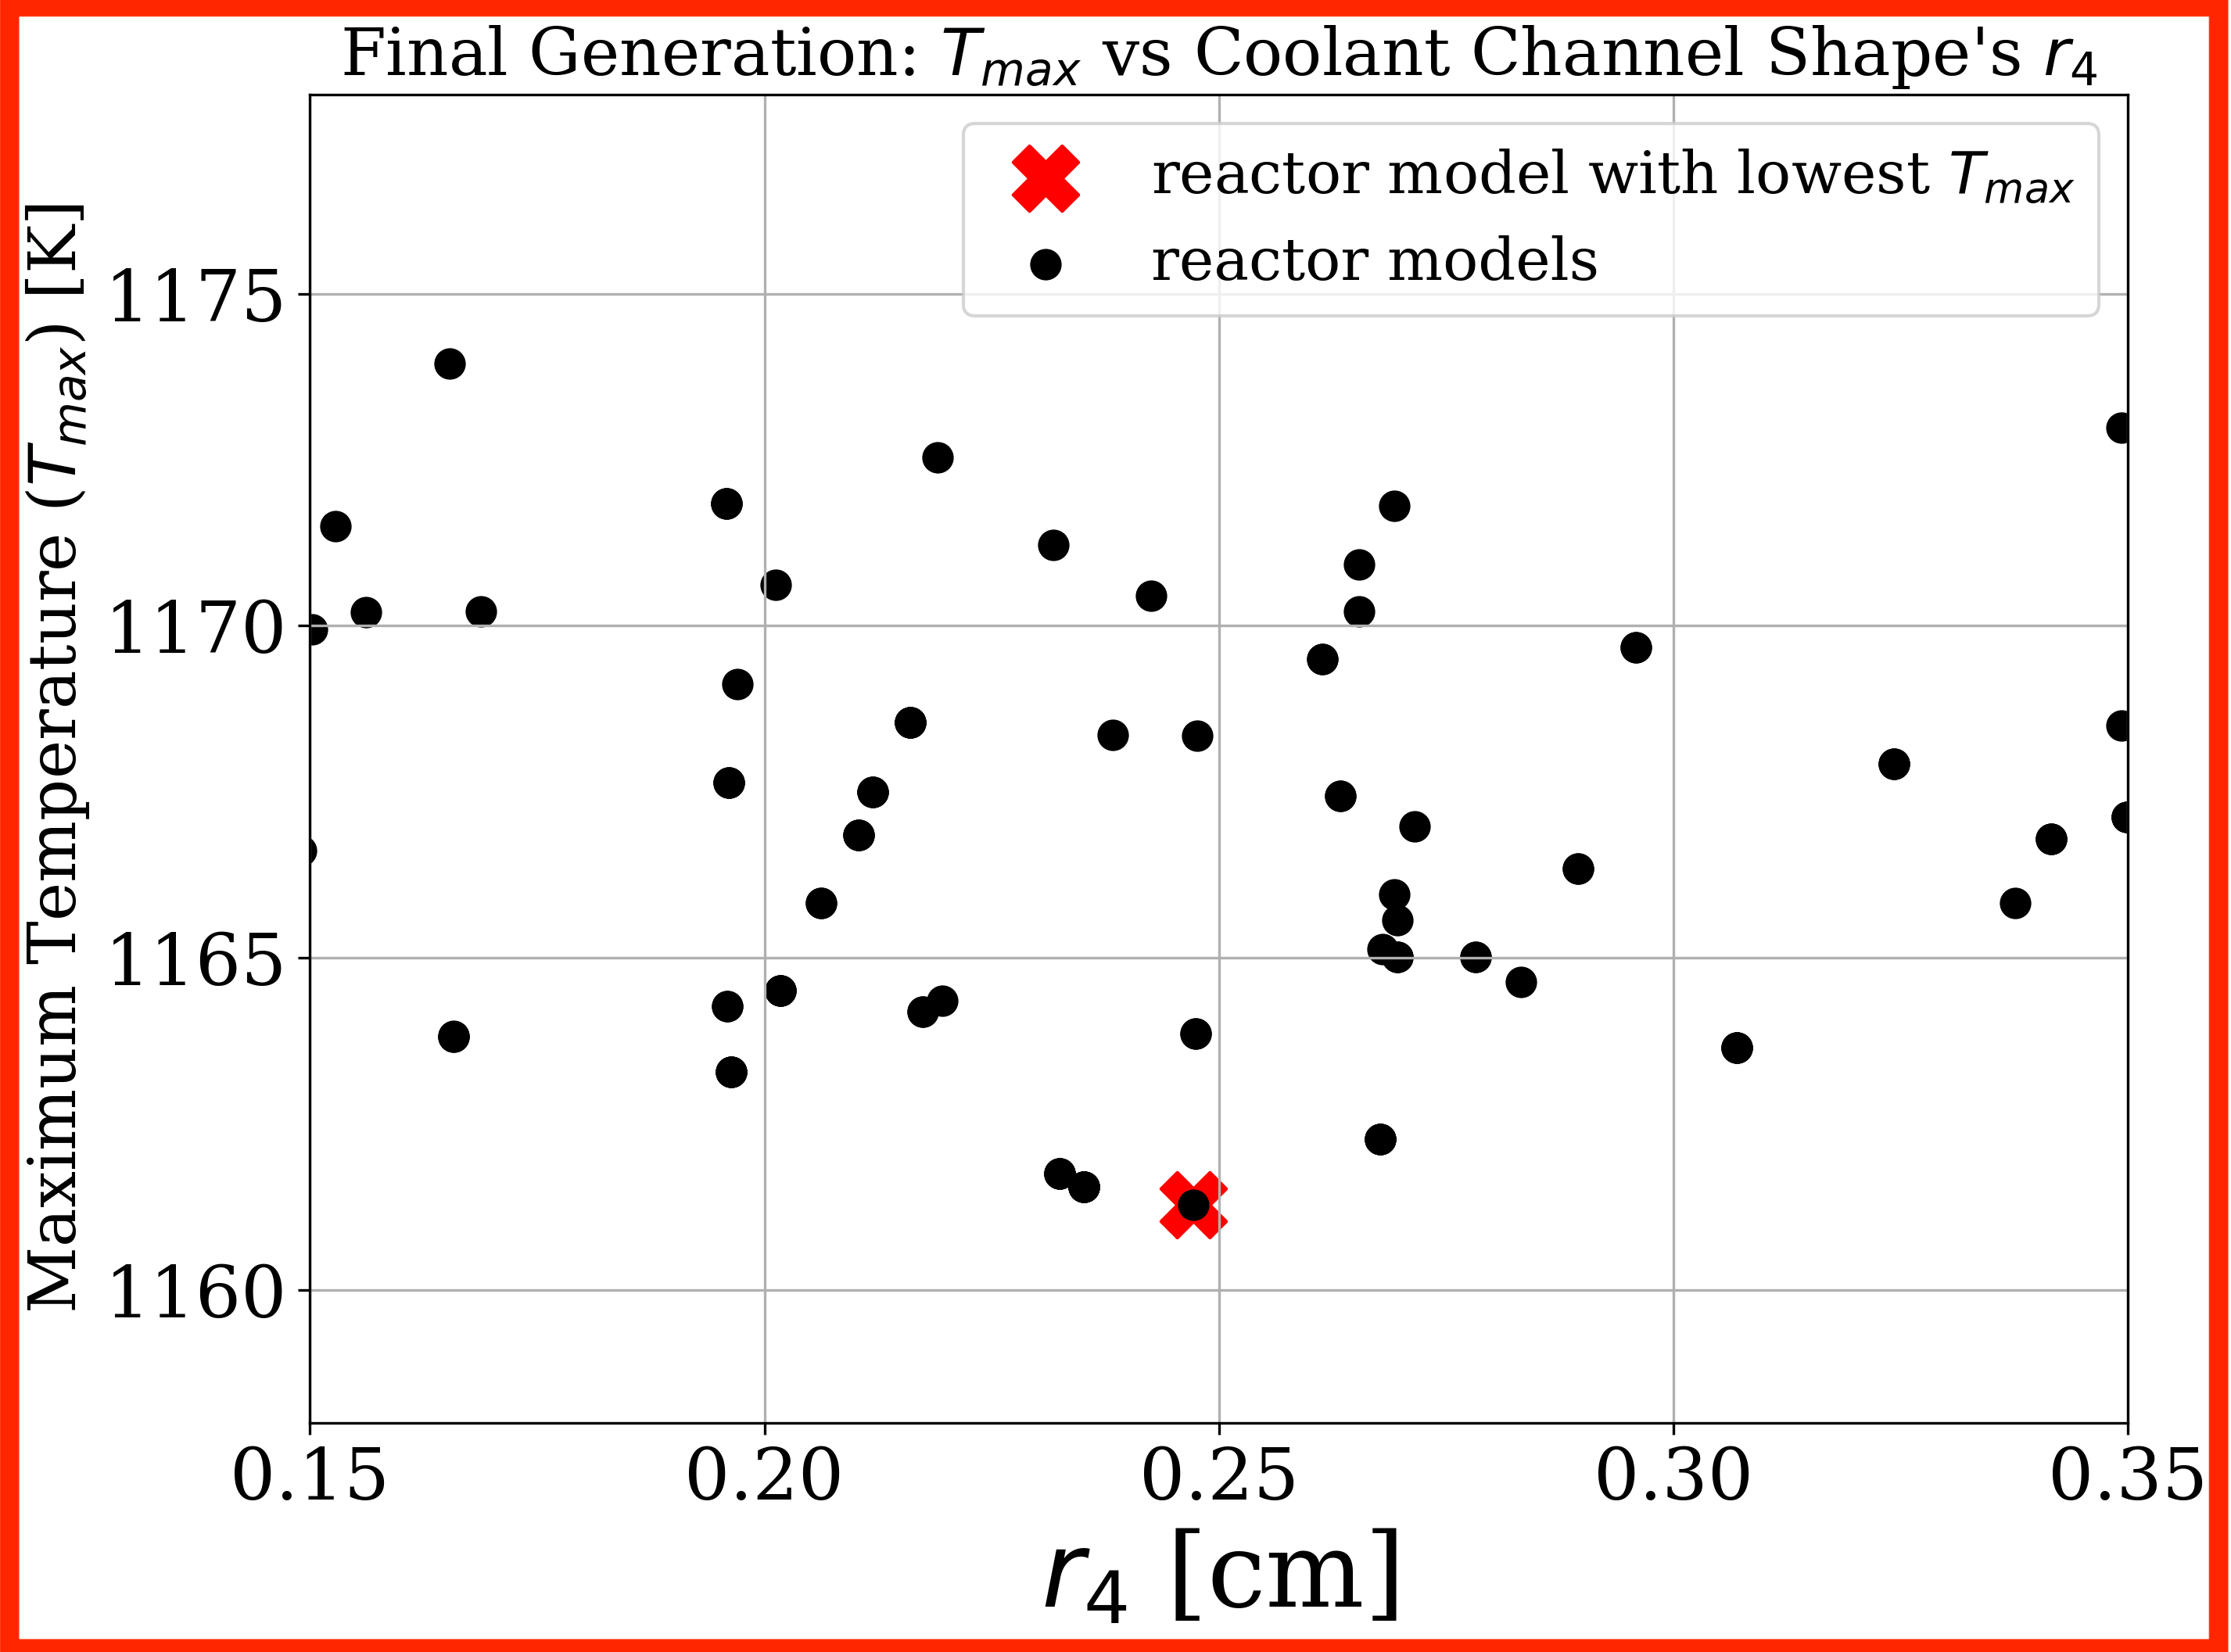
\includegraphics[width=\linewidth]{figures/a-1e-r4-pres-annotated.png}}
            \vspace{-0.5cm}
            \caption{Plot of $T_{max}$ against $r_4$.}
        \end{subfigure}
        \begin{subfigure}{0.3\textwidth}
            \only<1,3>{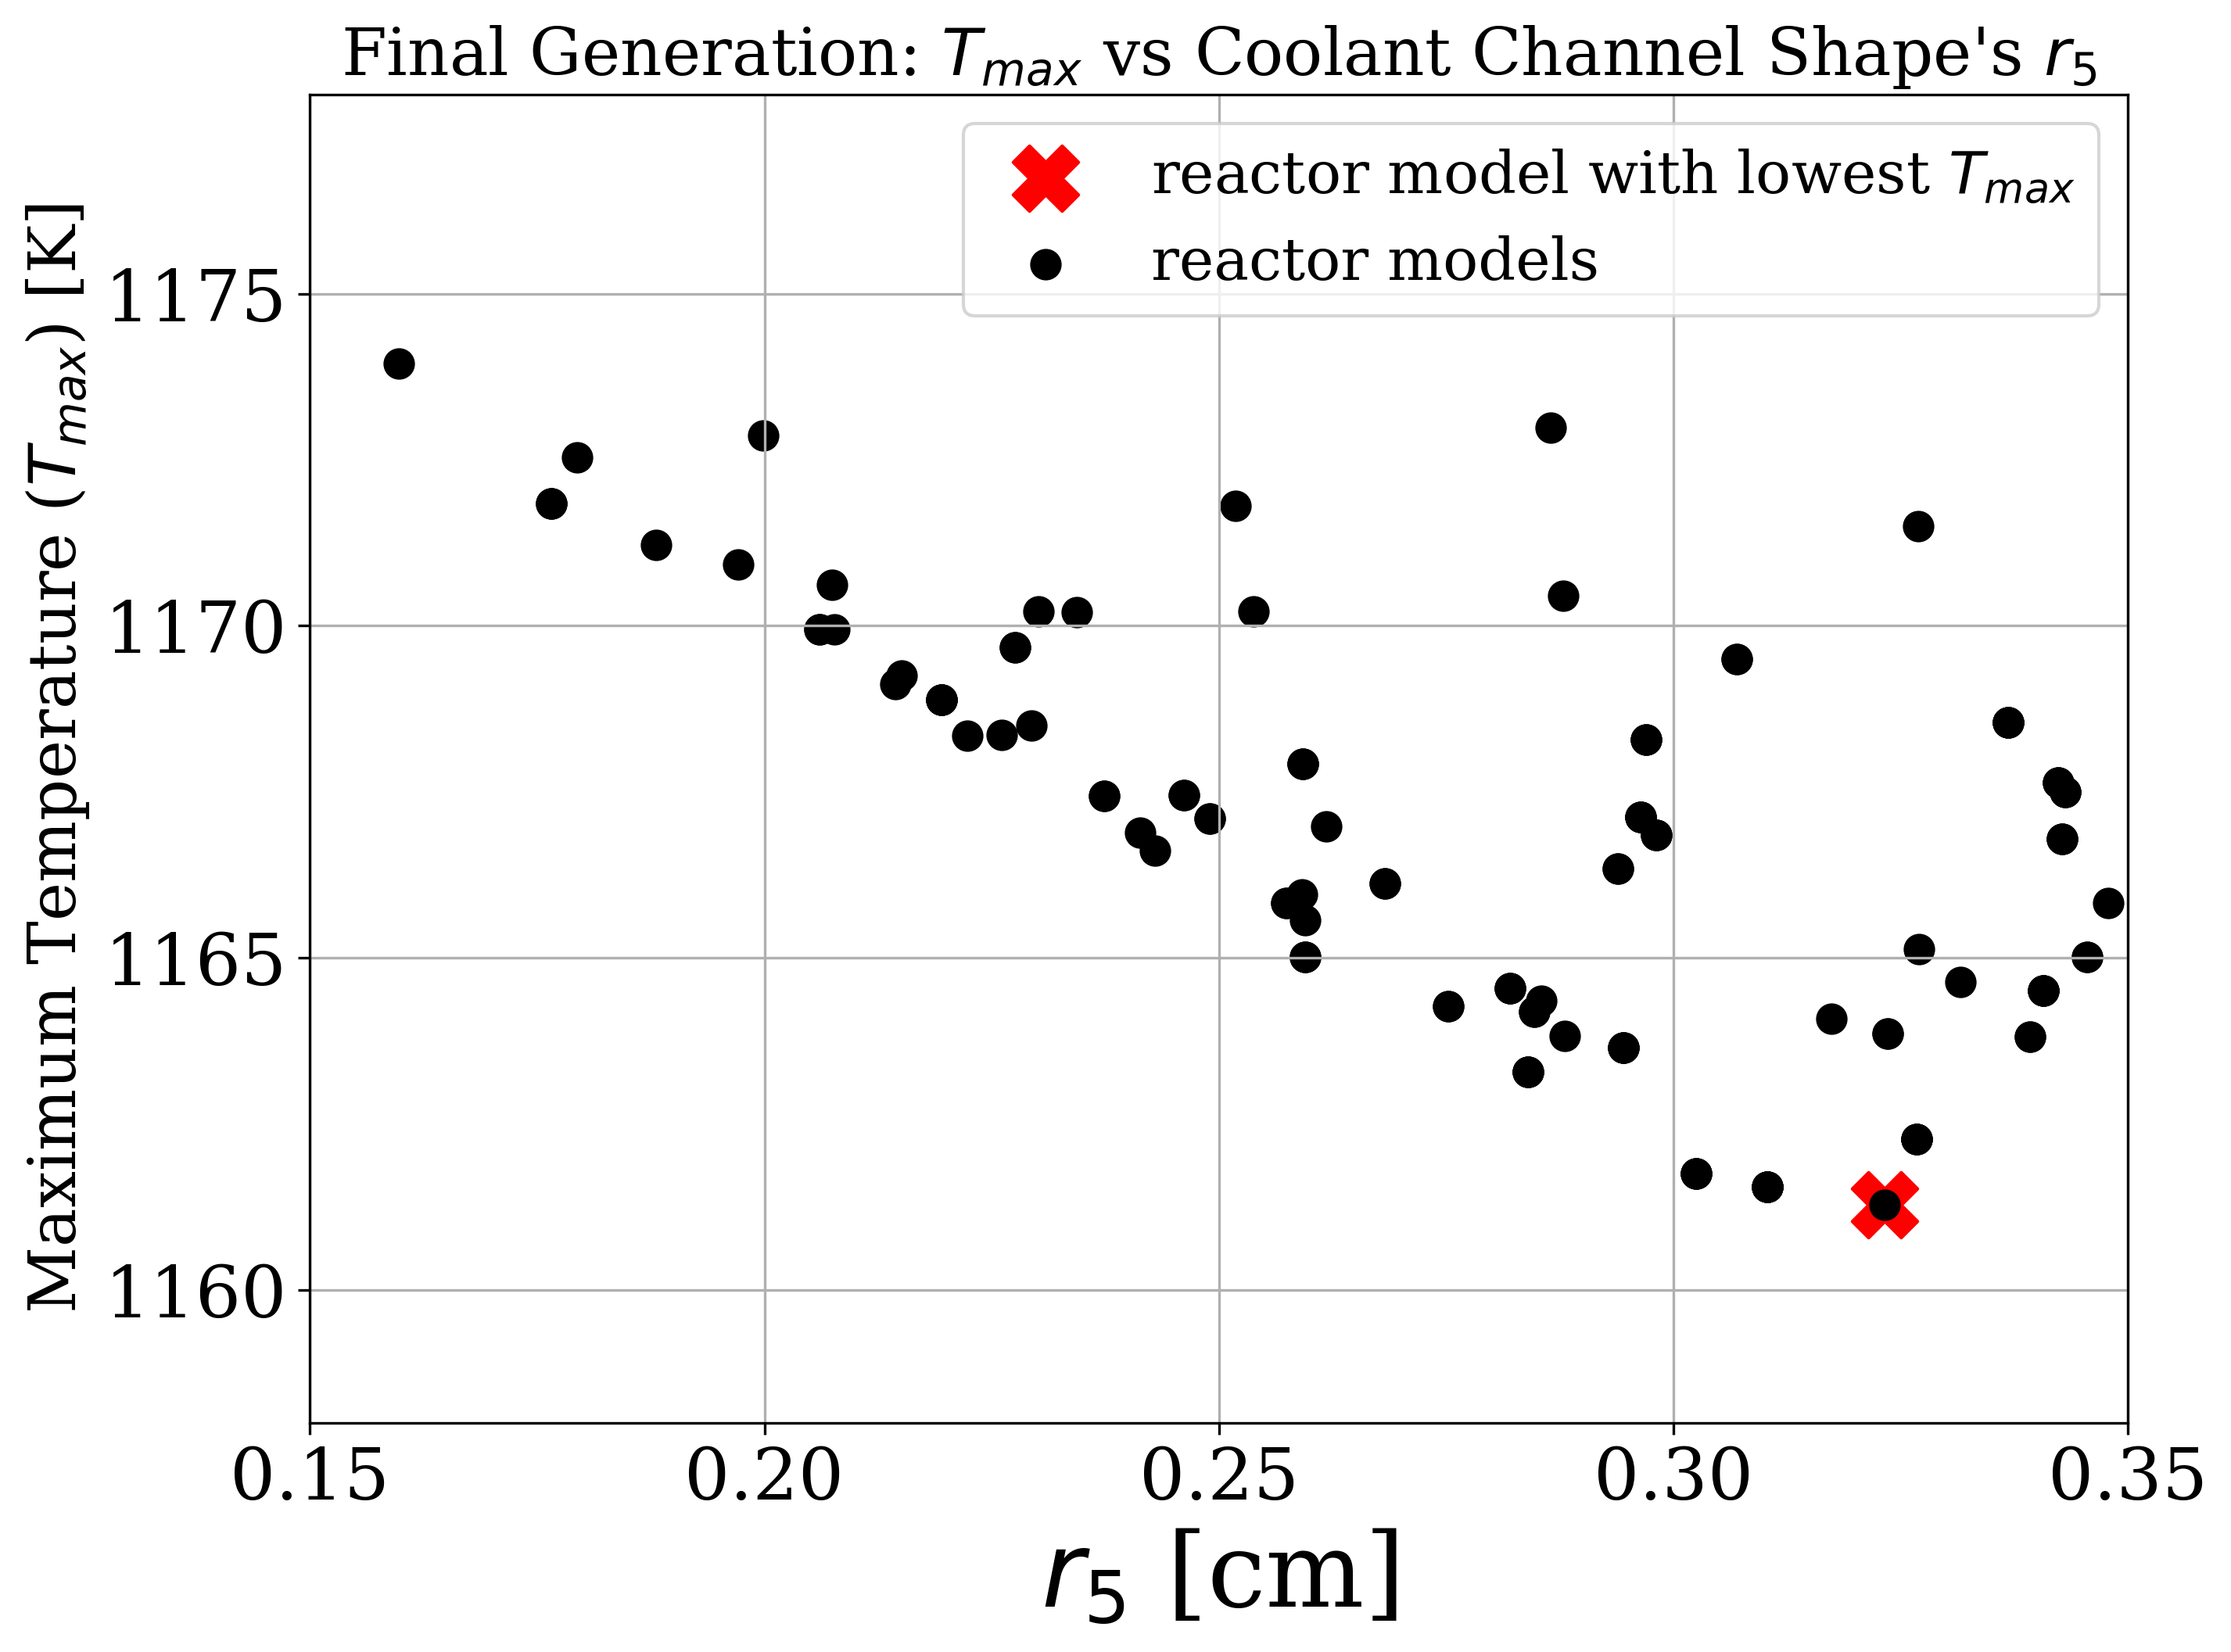
\includegraphics[width=\linewidth]{figures/a-1e-r5-pres.png}}
            \only<2>{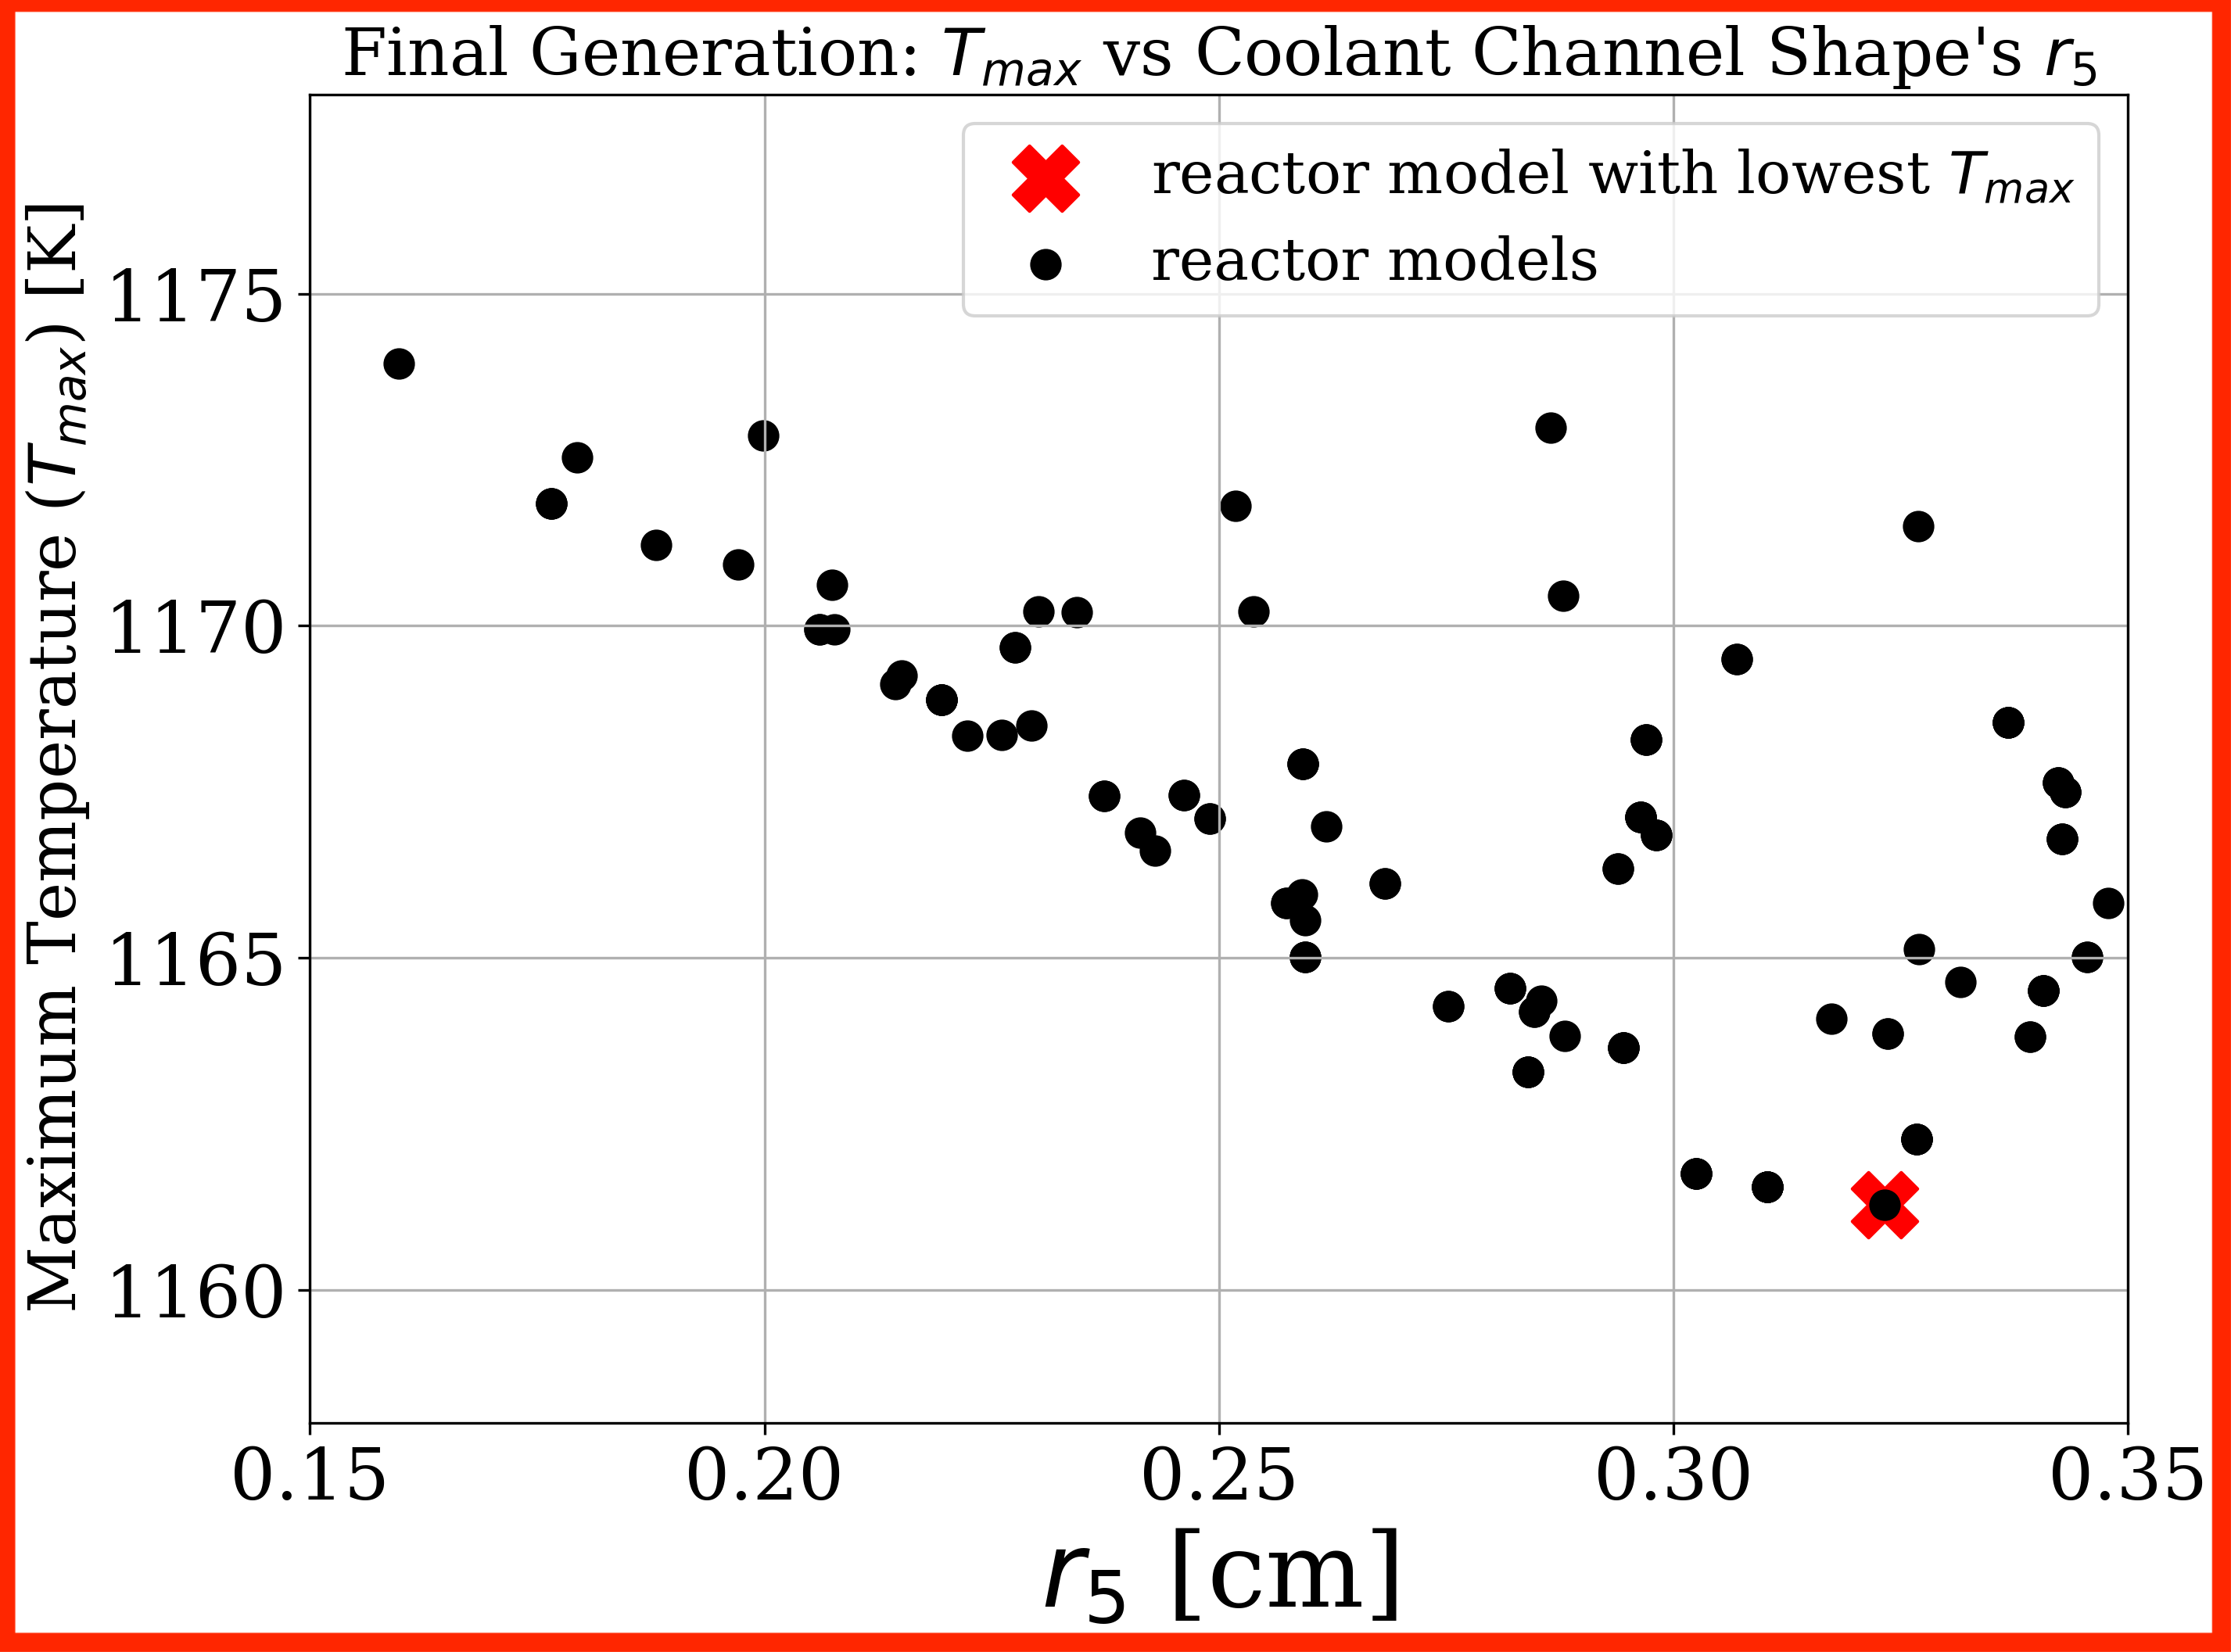
\includegraphics[width=\linewidth]{figures/a-1e-r5-pres-annotated.png}}
            \vspace{-0.5cm}
            \caption{Plot of $T_{max}$ against $r_5$.}
        \end{subfigure}
    \end{figure}
    \only<1>{\textbf{Plots demonstrate if $T_{max}$ is correlated with each radius values.}}
    \only<2>{\textbf{There is a strong negative linear correlation between $T_{max}$ and 
    $r_1$ and $r_5$.}}
    \only<3>{\textbf{Random scattering shows that $T_{max}$ has a weak correlation with 
    $r_2$, $r_3$, $r_4$}.}
\end{frame}

\begin{frame}
    \frametitle{AHTR One-Third Assembly Simulation a-1e Results}
    \begin{figure}
        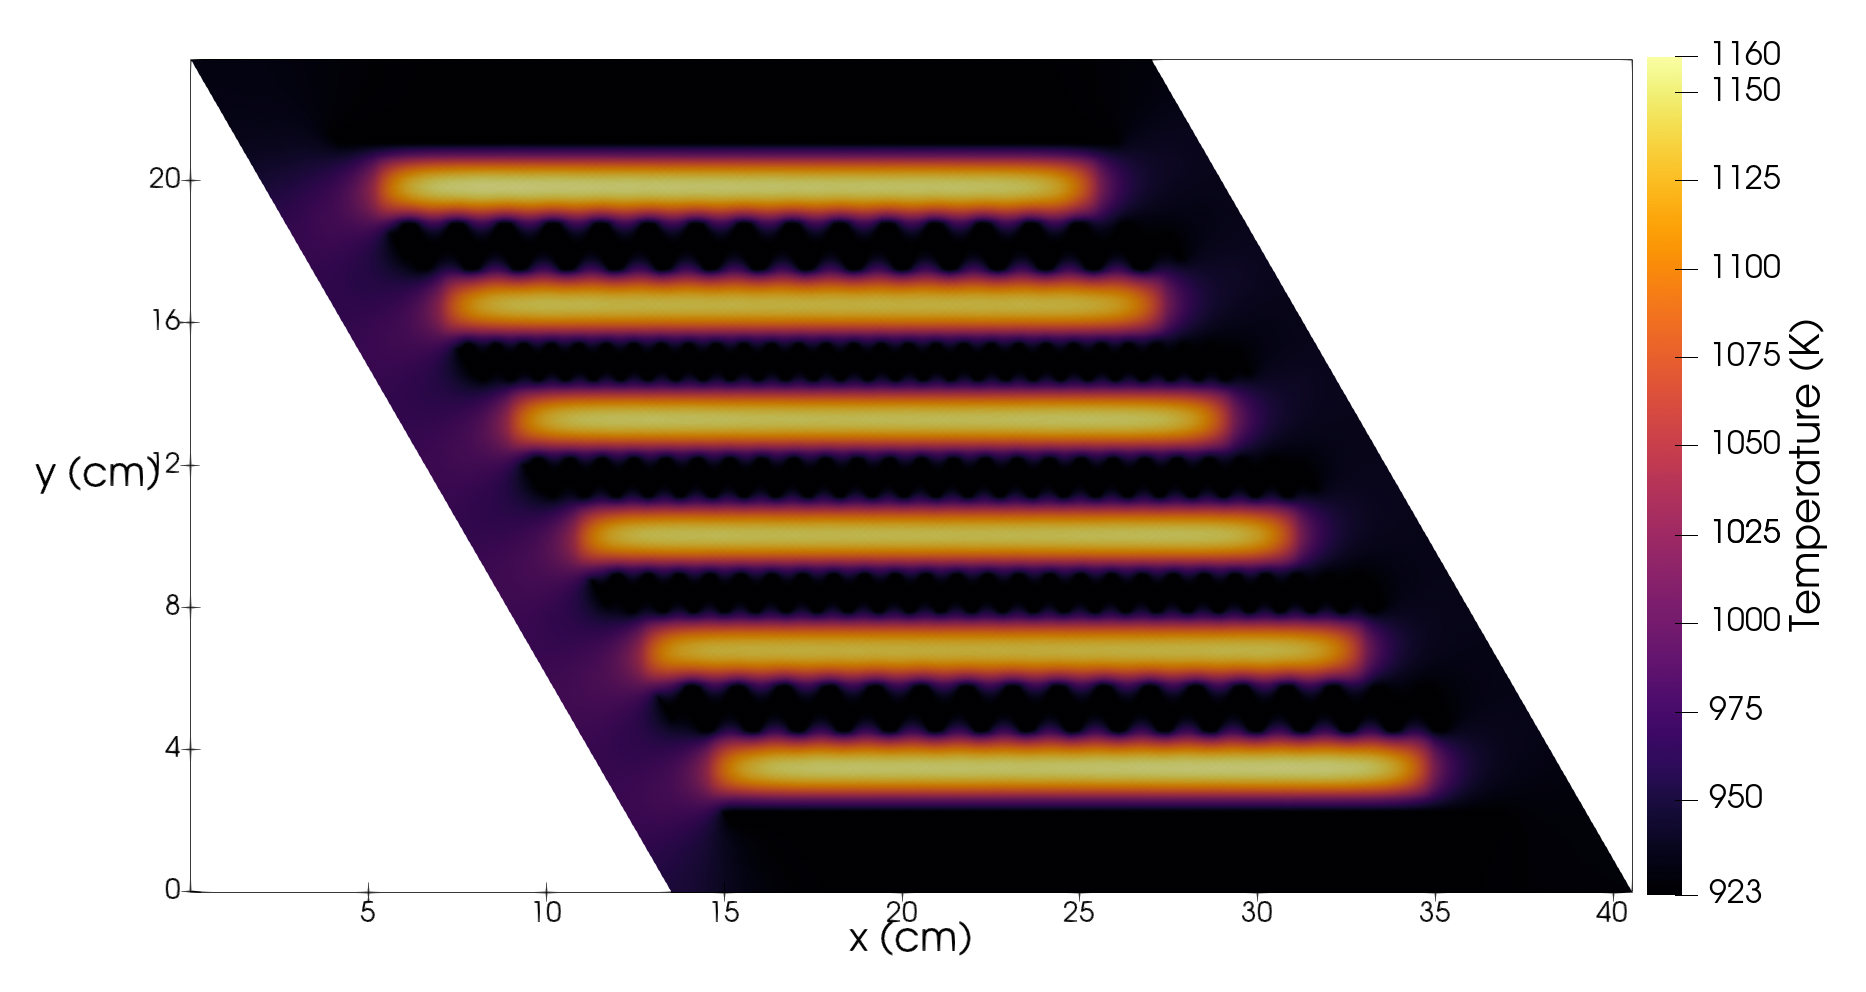
\includegraphics[width=0.59\linewidth]{../docs/figures/a-1e-temp-distribution-2d.png} 
        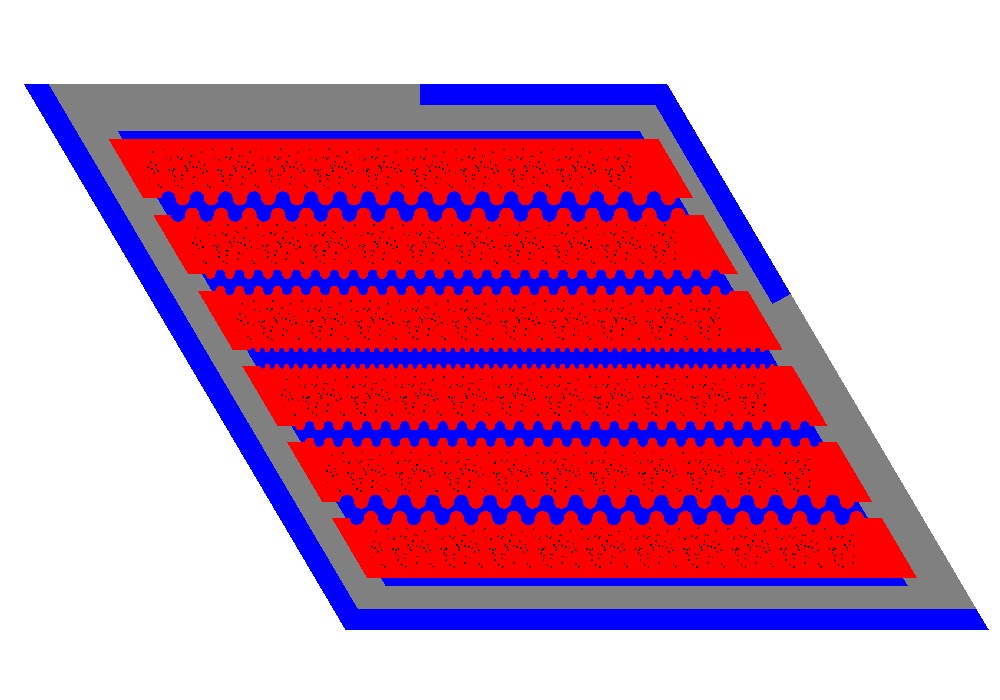
\includegraphics[width=0.4\linewidth]{../docs/figures/coolant-channel-shape-assem.png} 
        \caption{Temperature Distribution in the reactor model with the lowest $T_{max}$.}
    \end{figure}

    To minimize $T_{max}$, ROLLO maximized $r_1$ and $r_5$ to enable enhanced cooling 
    in the top and bottom graphite planks where the temperature peaking was occuring.

    \visible<2->{\begin{tcolorbox}[colback=illiniorange,colframe=illiniorange!50!black]
    \textbf{FLiBe channels located closest to temperature peaks shows a \\ negative 
    correlation with $T_{max}$.}
    \end{tcolorbox}}
\end{frame}

\begin{frame}
    \frametitle{Single-Objective Optimization Major Takeaways}
    \visible<1->{\textbf{Minimize $PF_{total}$ Objective} 
    \begin{itemize}
        \item Driven by maximizing total fission reaction rate
        \item Influences oscillations in TRISO's spatial distribution
        \item No correlation with coolant channel shape  
    \end{itemize}}

    \vspace{0.2cm}
    \visible<2->{\textbf{Minimize $T_{max}$ Objective}
    \begin{itemize}
        \item The minimize $T_{max}$ objective prefers a flatter TRISO distribution 
        \item FLiBe channels located closest to temperature peaks shows a negative 
        correlation with $T_{max}$
    \end{itemize}}

    \vspace{0.2cm}
    \visible<3->{\textbf{Minimize $PPF_{fuel}$ Objective} 
    \begin{itemize}
        \item Driven by flattening thermal flux distribution
        \item Influences oscillations in TRISO's spatial distribution
        \item No correlation with coolant channel shape  
    \end{itemize}}
\end{frame}

\begin{frame}
    \frametitle{AHTR One-Third Assembly Simulation a-2b Results}
    \begin{columns}[t]
        \only<1>{\begin{column}{0.35\textwidth}
        \begin{block}{Simulation a-2b}
        \begin{itemize}
        \item I vary $PF_{total}$ and \textbf{a, b, c, d, e f} 
        ($\rho_{TRISO}(\vec{x}, \vec{y}$)) 
        \item Minimize $PF_{total}$ and $PPF_{fuel}$ objectives
        \item 5 generations 
        \item 128 reactor models per gen  
        \item Total runtime: 492 Theta node-hours
        \end{itemize}
        \end{block}
        \end{column}}
        \only<2>{\begin{column}{0.5\textwidth}
            \begin{block}{Pareto Front}
            \begin{itemize}
                \item Multi objective optimization with competing objectives will return 
                \textbf{multiple optimal solutions that meet each objective to varying 
                degrees}
                \item For each reactor model on the pareto front, \textbf{none of the 
                objective values can be improved without degrading another}
            \end{itemize}
        \end{block}
        \end{column}}
        \only<3>{\begin{column}{0.35\textwidth}
            \vspace{-0.4cm}
            \begin{block}{Simulation a-2b}
            \begin{itemize}
            \item The 12 reactor models on simulation a-2b's Pareto front have different 
            $PF_{total}$ and $\rho_{TRISO}(\vec{r})$ depending on \textbf{extent each
            objective is minimized.}
            \item Reactor 11 = lowest $PF_{total}$, highest $PPF_{fuel}$
            \item Reactor 3 = lowest $PPF_{fuel}$, highest $PF_{total}$
            \item Reactor 5 = minimizes both objectives to an equal extent 
            \end{itemize}
            \end{block}
            \end{column}}
    \only<1,3>{    
        \begin{column}{0.65\textwidth}
        \textbf{Simulation a-2b's Pareto front shows the tradeoff between 
        minimize $PF_{total}$ and $PPF_{fuel}$ objectives.}
        \begin{figure}
            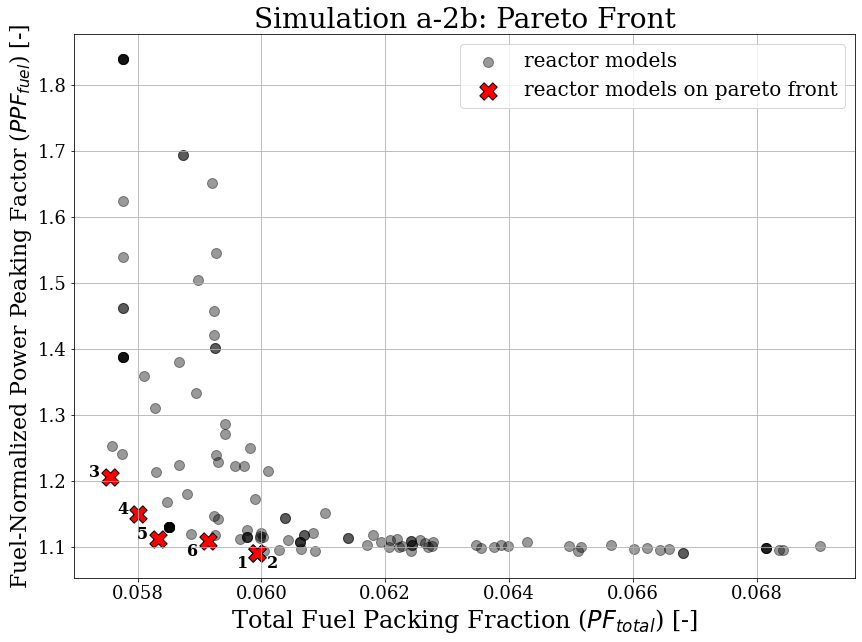
\includegraphics[width=\linewidth]{../docs/figures/assem-obj-2-pfppf-pareto.png} 
        \end{figure}
    \end{column}}
    \only<2>{    
        \begin{column}{0.5\textwidth}
        \begin{figure}
            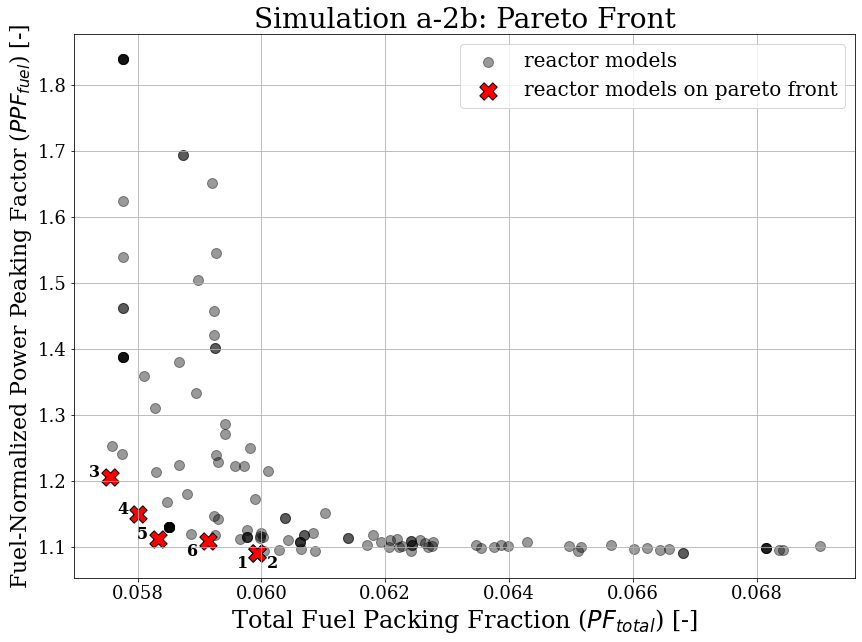
\includegraphics[width=\linewidth]{../docs/figures/assem-obj-2-pfppf-pareto.png} 
        \end{figure}
    \end{column}}
    \end{columns}

    \vspace{0.4cm}
    \only<2>{\textbf{Successful multi-objective optimization finds a wide spread of 
    reactor models on their Pareto fronts}}
\end{frame}

\begin{frame}
    \frametitle{AHTR One-Third Assembly Simulation a-2b Results}
    \centering
    \textbf{TRISO Distributions for reactor models' on the Pareto front.}

    \vspace{0.2cm}
    \begin{figure}
        \only<1>{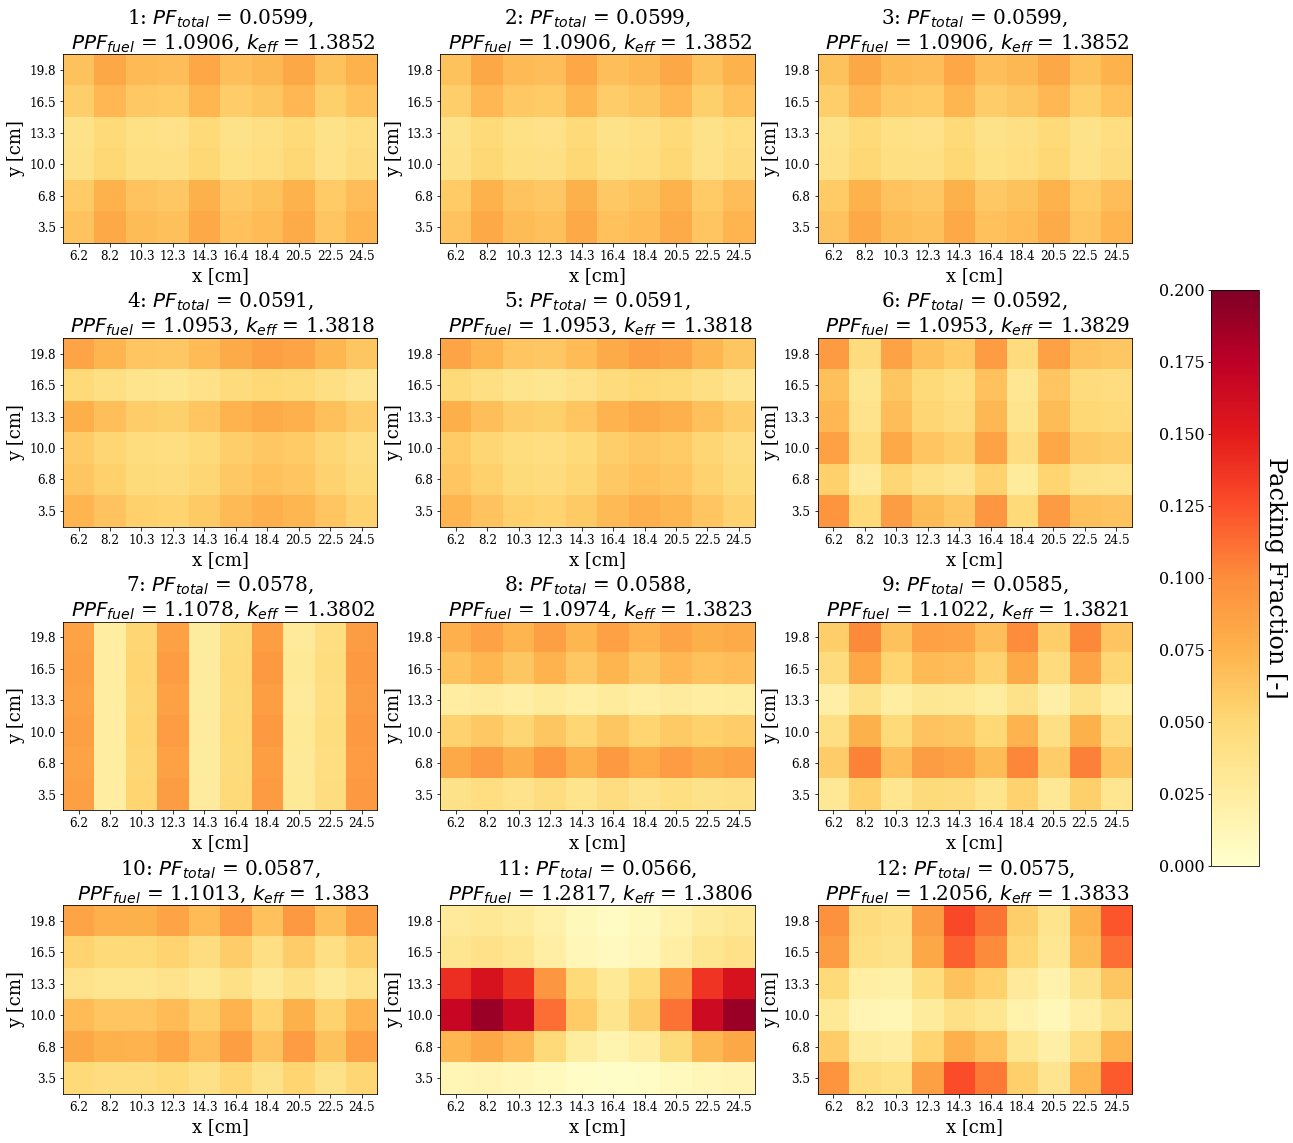
\includegraphics[width=0.85\linewidth]{../docs/figures/assem-obj-2-pfppf-pareto-distr.png}}
        \only<2>{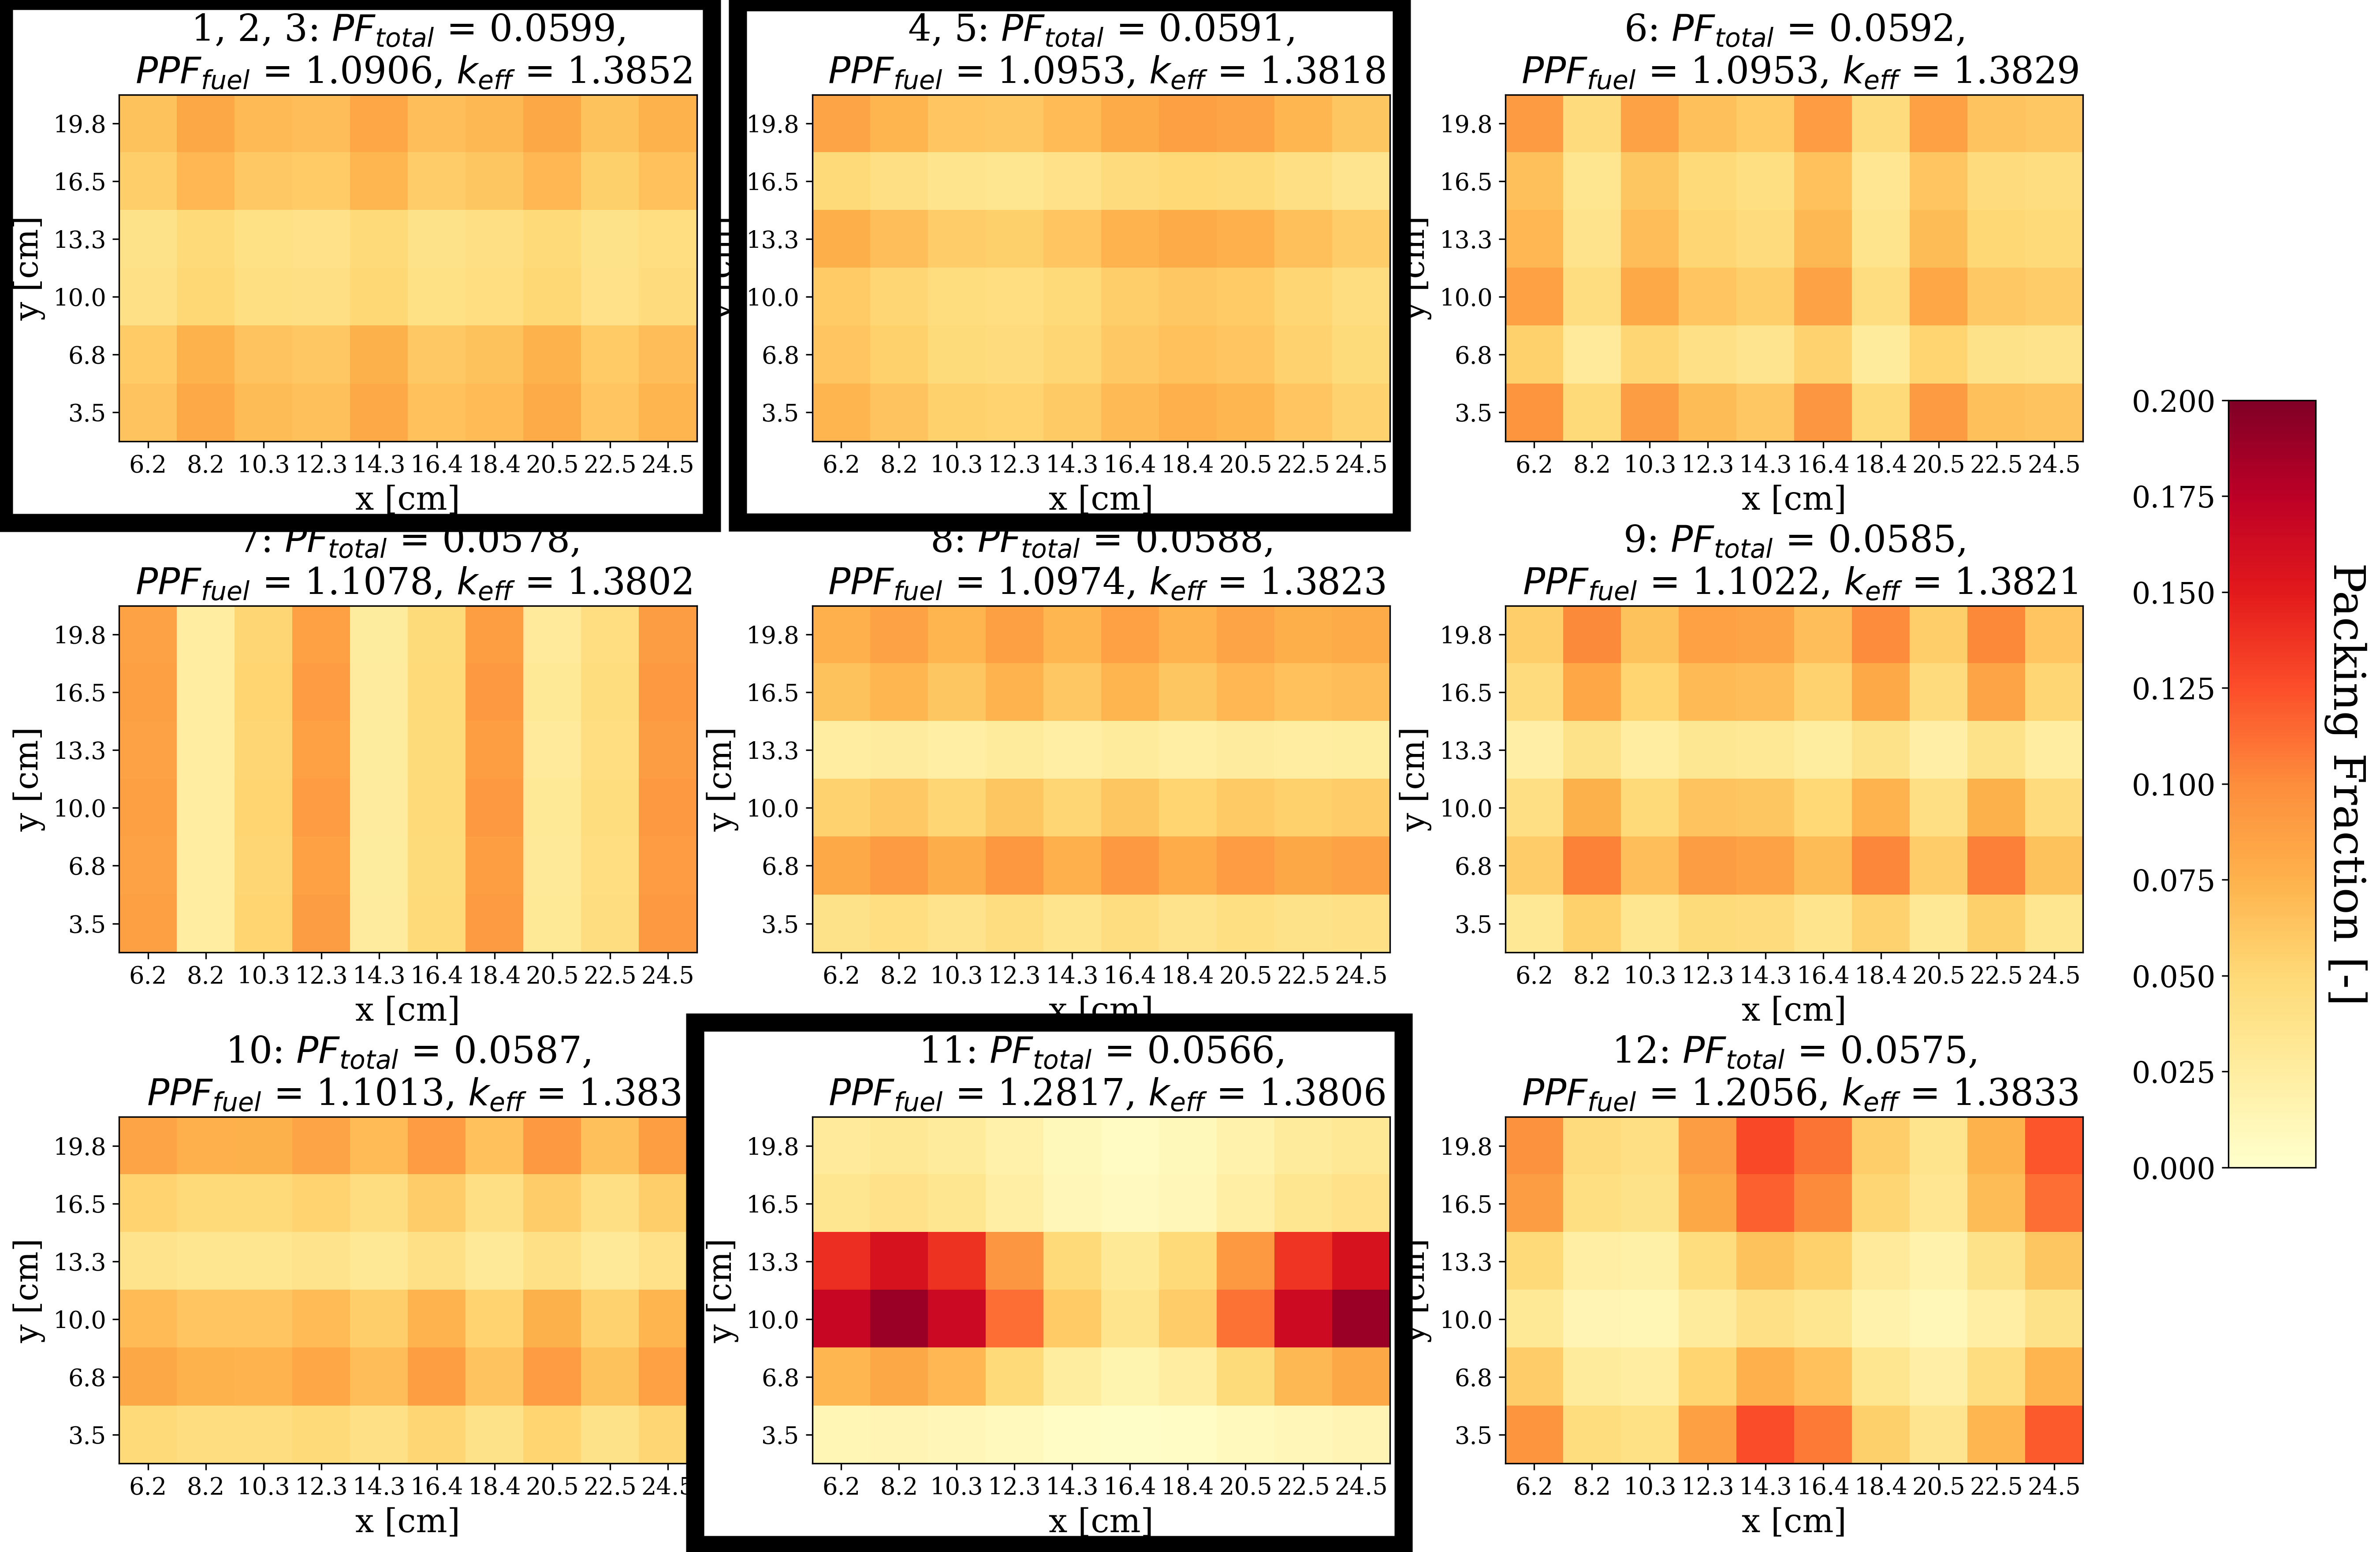
\includegraphics[width=0.85\linewidth]{figures/assem-obj-2-pfppf-pareto-distr-annotated.png}}
    \end{figure}
\end{frame}

\begin{frame}
    \frametitle{AHTR One-Third Assembly Simulation a-2b Results}
    \begin{figure}
        \centering
        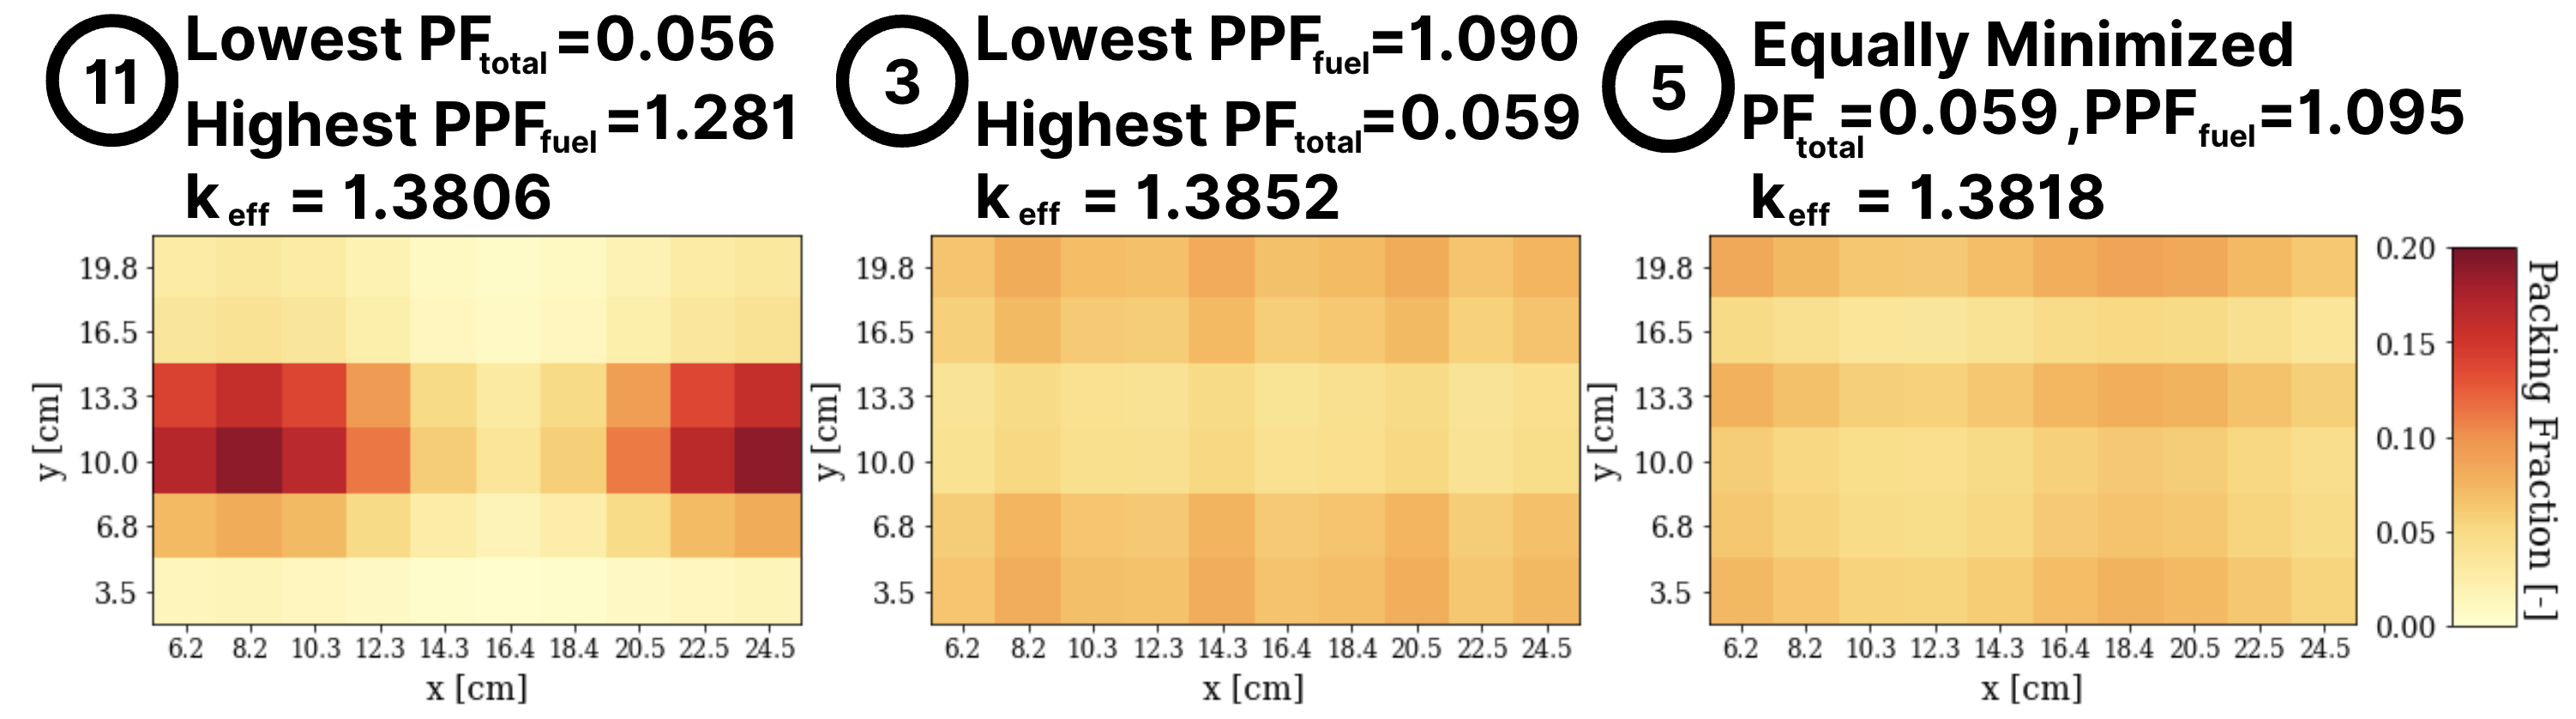
\includegraphics[width=\linewidth]{figures/a-2b-comparison-reactors.png}
    \end{figure}

    Minimize $PF_{total}$ is driven by \textbf{maximizing total fission reaction rate} 
    \begin{itemize}
        \visible<1->{\item Reactor 11 with $PF_{total} = 0.056$ and reactor model 5 with 
        $PF_{total} = 0.059$ have the similar $k_{eff}$ and total fission reaction rate} 
        \visible<2->{\item Reactors 11 TRISO distribution enables it to achieve the 
        same $k_{eff}$ as reactor 5 despite having a lower $PF_{total}$}
        \visible<3->{\item \textbf{Reactor 11 TRISO distribution minimizes spatial 
        self-shielding effects}}
    \end{itemize}
\end{frame}

\begin{frame}
    \frametitle{AHTR One-Third Assembly Simulation a-2b Results}
    \begin{figure}
        \centering
        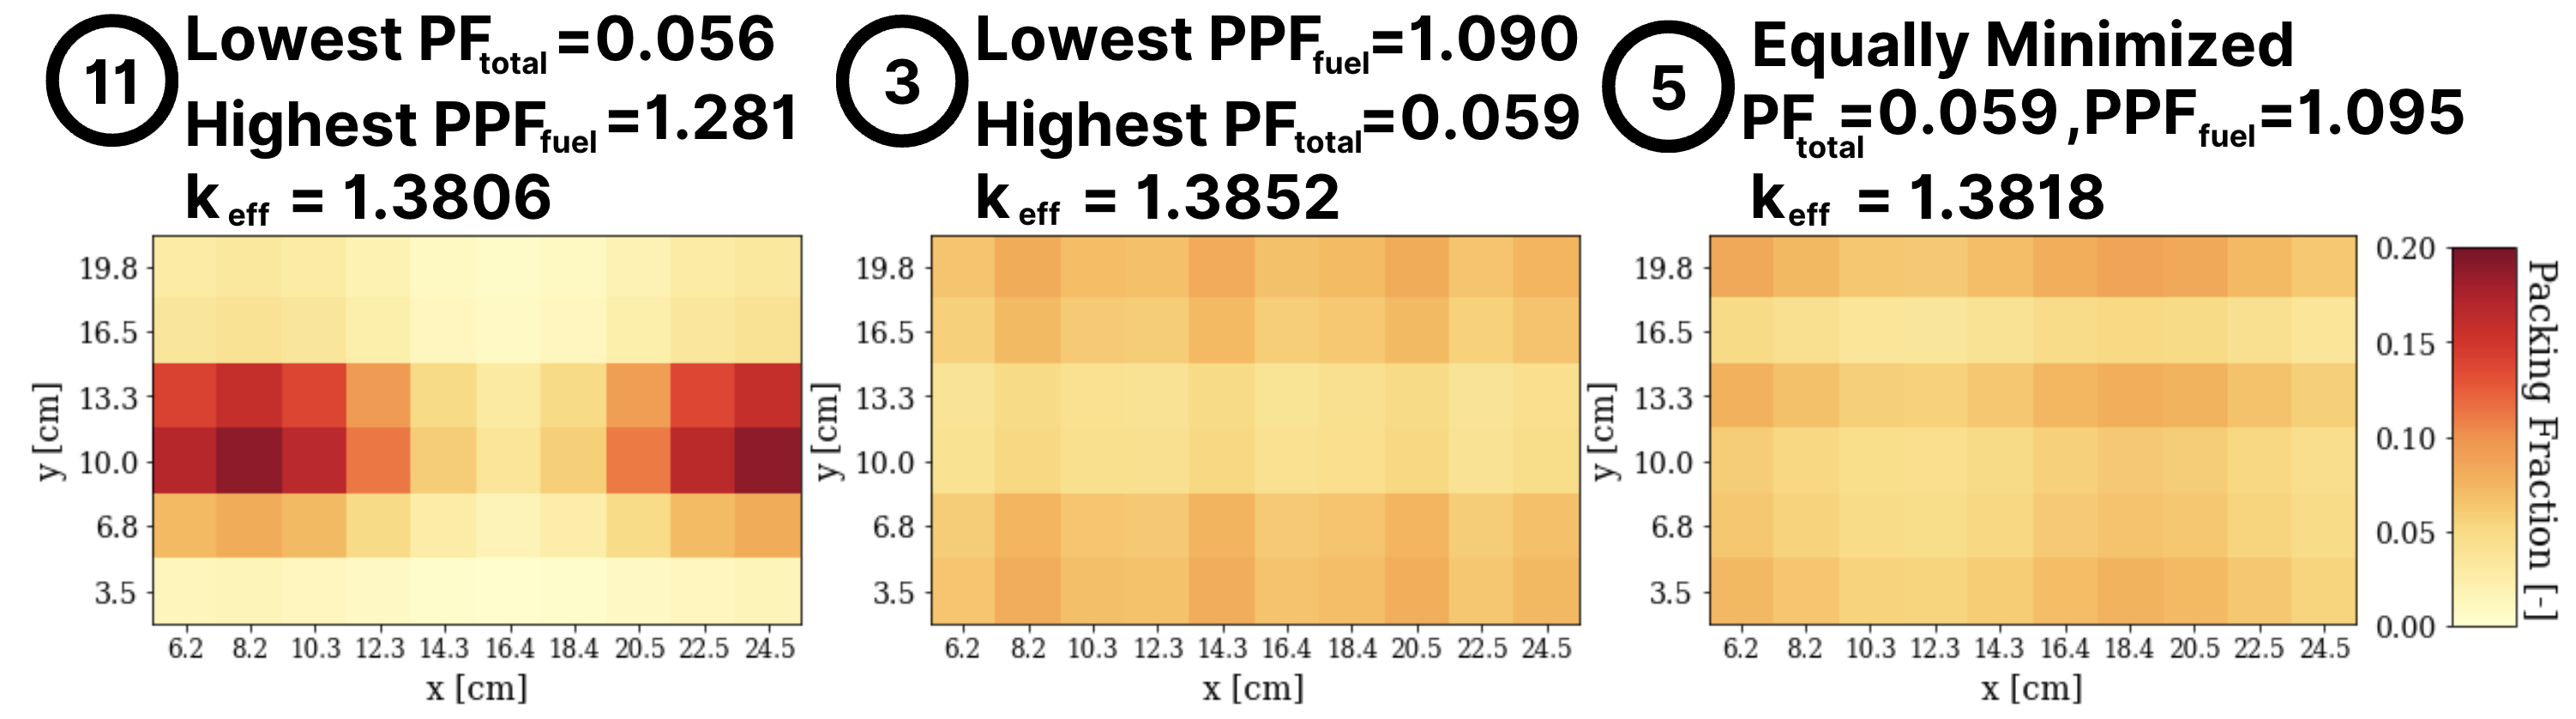
\includegraphics[width=\linewidth]{figures/a-2b-comparison-reactors.png}
    \end{figure}

    Minimize $PPF_{fuel}$ objective is driven by \textbf{flattening thermal 
    flux distribution}  
    \begin{itemize}
        \item Flattest to least flat thermal flux: reactor model 
                $3 \rightarrow 5 \rightarrow 11$
        \item \textbf{Reactor model 3 with lowest $PPF_{fuel}$ has flattest flux}
    \end{itemize}

    \begin{tcolorbox}[colback=illiniorange,colframe=illiniorange!50!black]
        Minimize $PF_{total}$ and Minimize $PPF_{fuel}$ objectives 
        influence each other resulting in \textbf{unexpected TRISO distributions at 
        different $PF_{total}$ values}. 
    \end{tcolorbox}
\end{frame}

\begin{frame}
    \frametitle{AHTR One-Third Assembly Simulation a-3b Results}
    \begin{columns}
    \begin{column}{0.35\textwidth}
        \begin{block}{Simulation a-3b}
            \begin{itemize}
            \item Vary $PF_{total}$, \textbf{a, b, c, d, e f} ($\rho_{TRISO}(\vec{x}, 
            \vec{y}$)), and $r_1, r_2, r_3, r_4, r_5$ (coolant channel shape) 
            \item Minimize all three objectives: $PF_{total}$, $T_{max}$ and $PPF_{fuel}$.
            \item 6 generations 
            \item 128 reactor models per gen 
            \item Total runtime: 1528 Theta node-hours = 97792 real-time hours 
            \end{itemize}
            \end{block}
        \end{column}
    \begin{column}{0.7\textwidth}
    \begin{figure}
        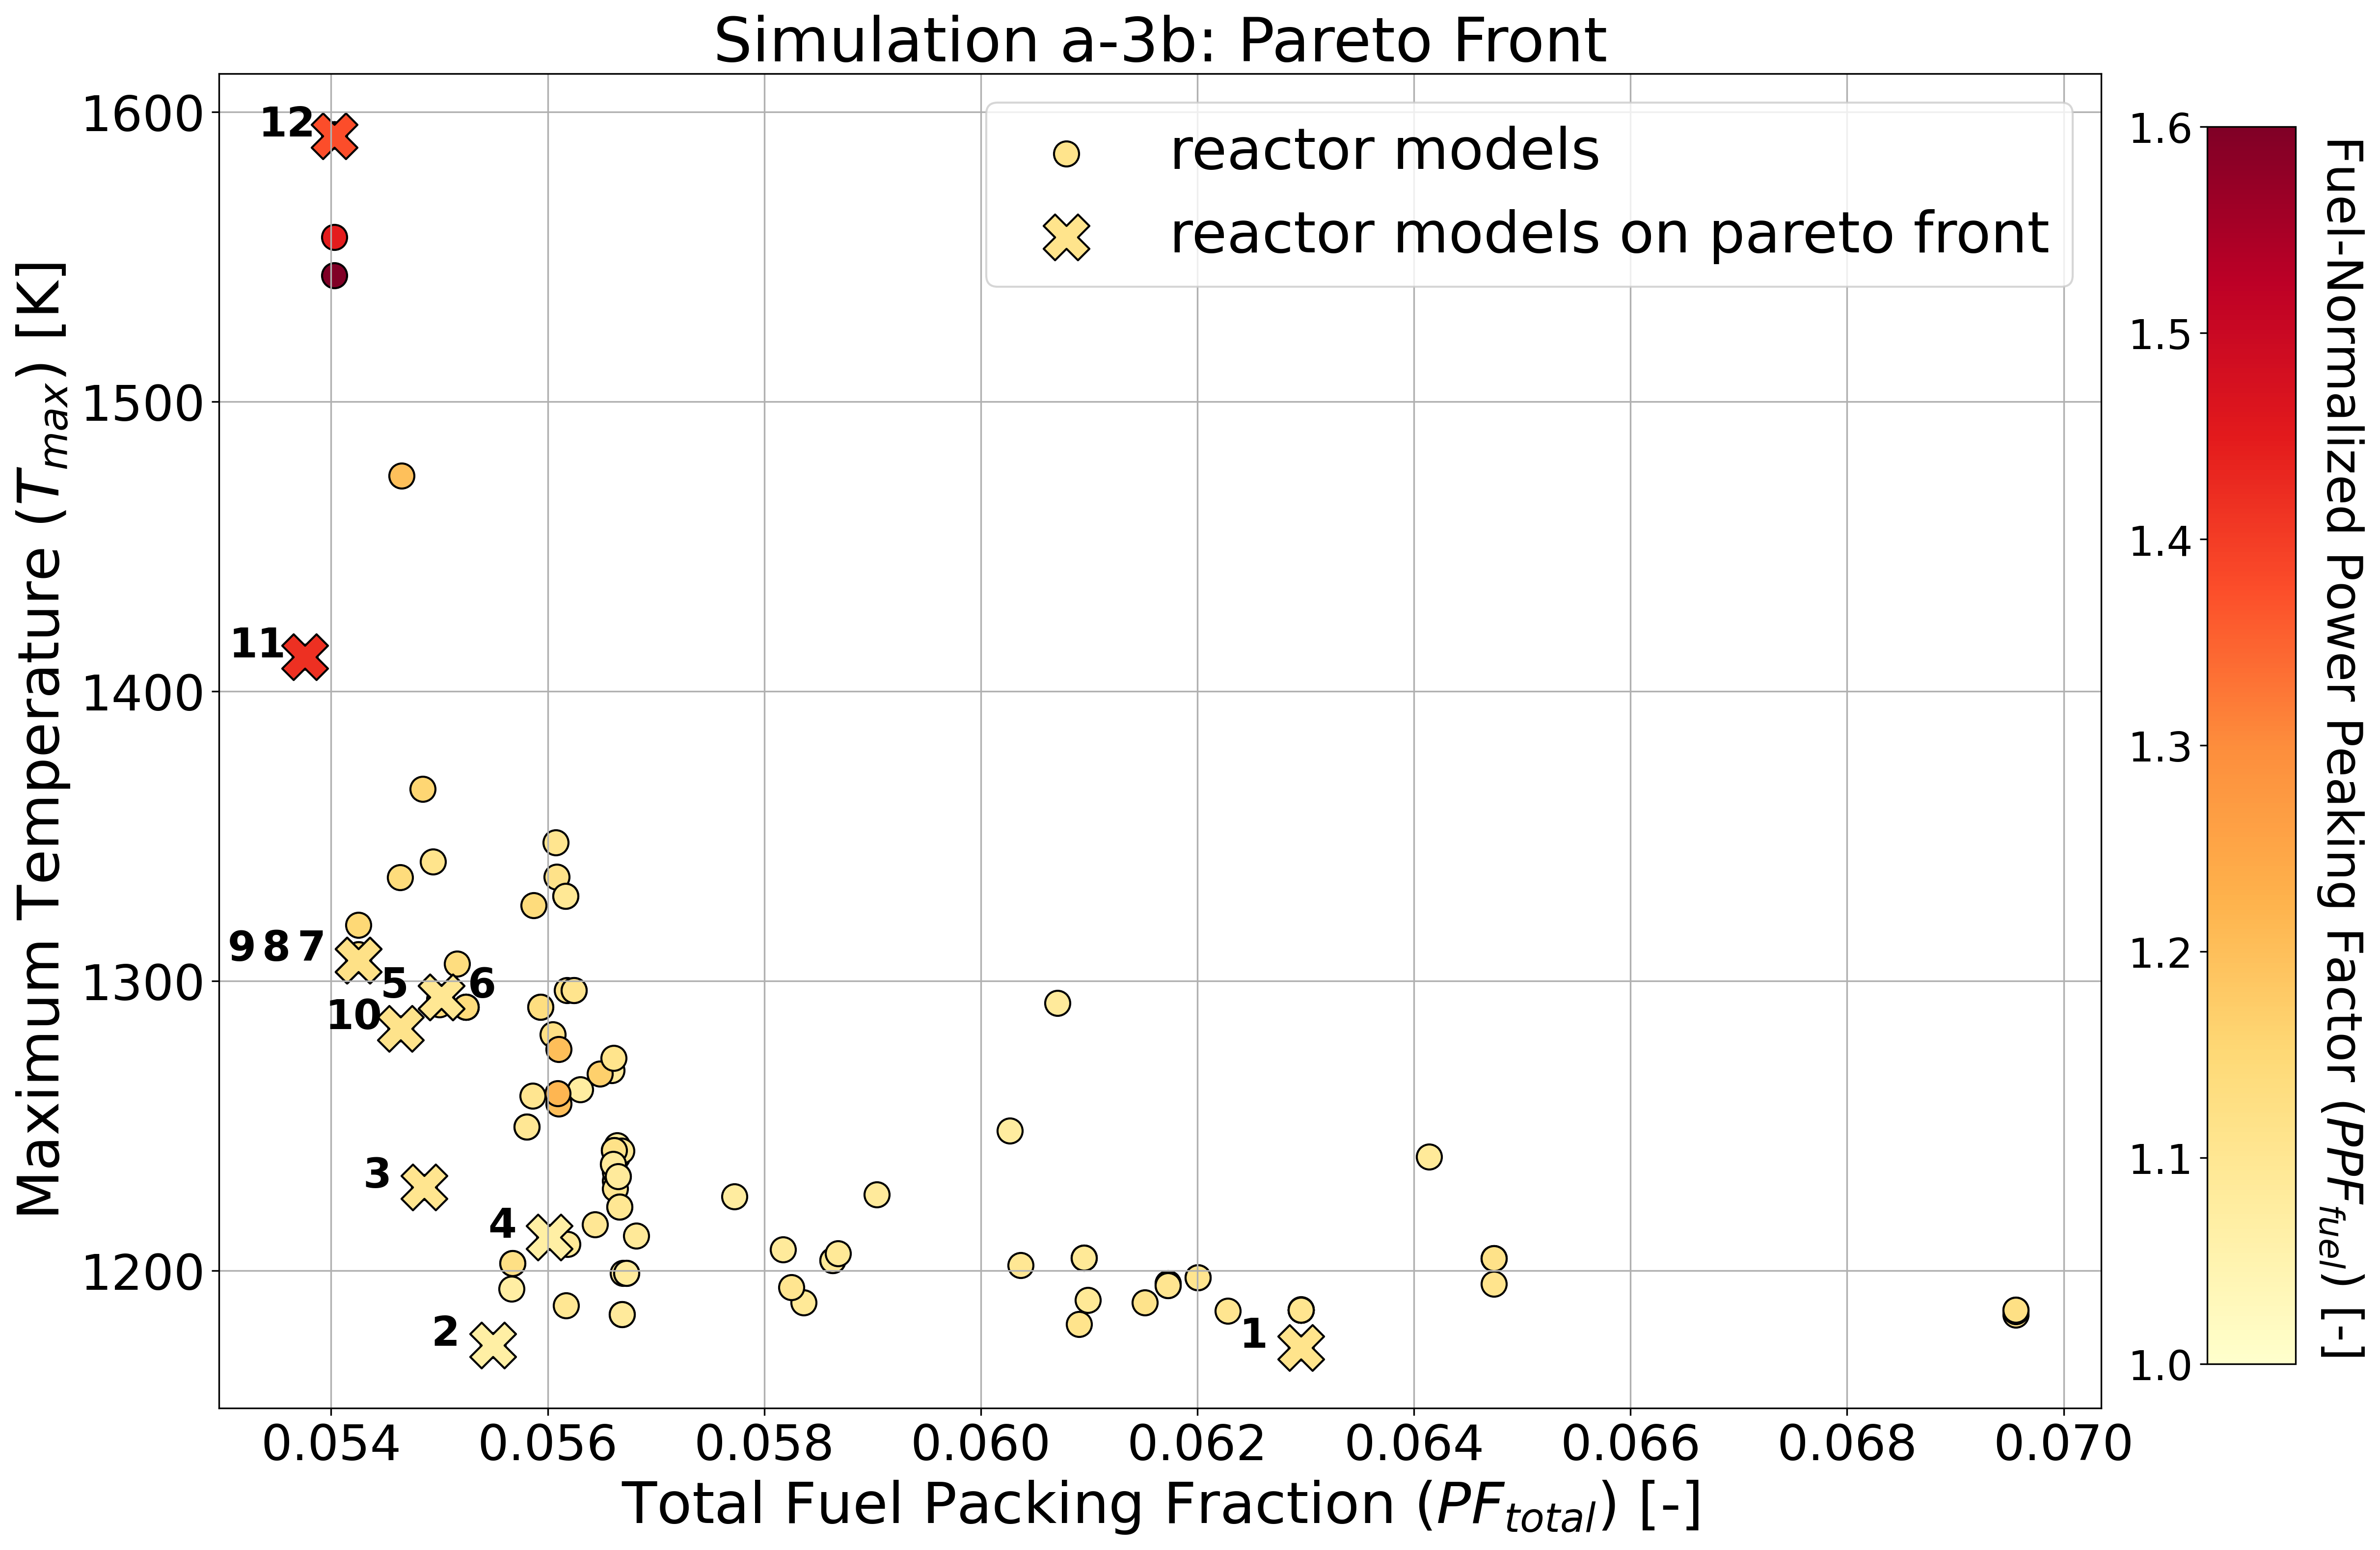
\includegraphics[width=\linewidth]{../docs/figures/assem-obj-3-all-2d.png} 
        \caption{Plot of final generation's reactor models' 
        $PF_{total}$ against $T_{max}$ against $PPF_{fuel}$ as a color dimension. 
        Crosses indicate the reactor models on the Pareto front.}
    \end{figure}
    \end{column}
\end{columns}
\end{frame}

\begin{frame}
    \frametitle{AHTR One-Third Assembly Simulation a-3b Results}
    \textbf{TRISO Distributions for reactor models' on the Pareto front.}

    \vspace{0.2cm}
    \begin{figure}
        \only<1>{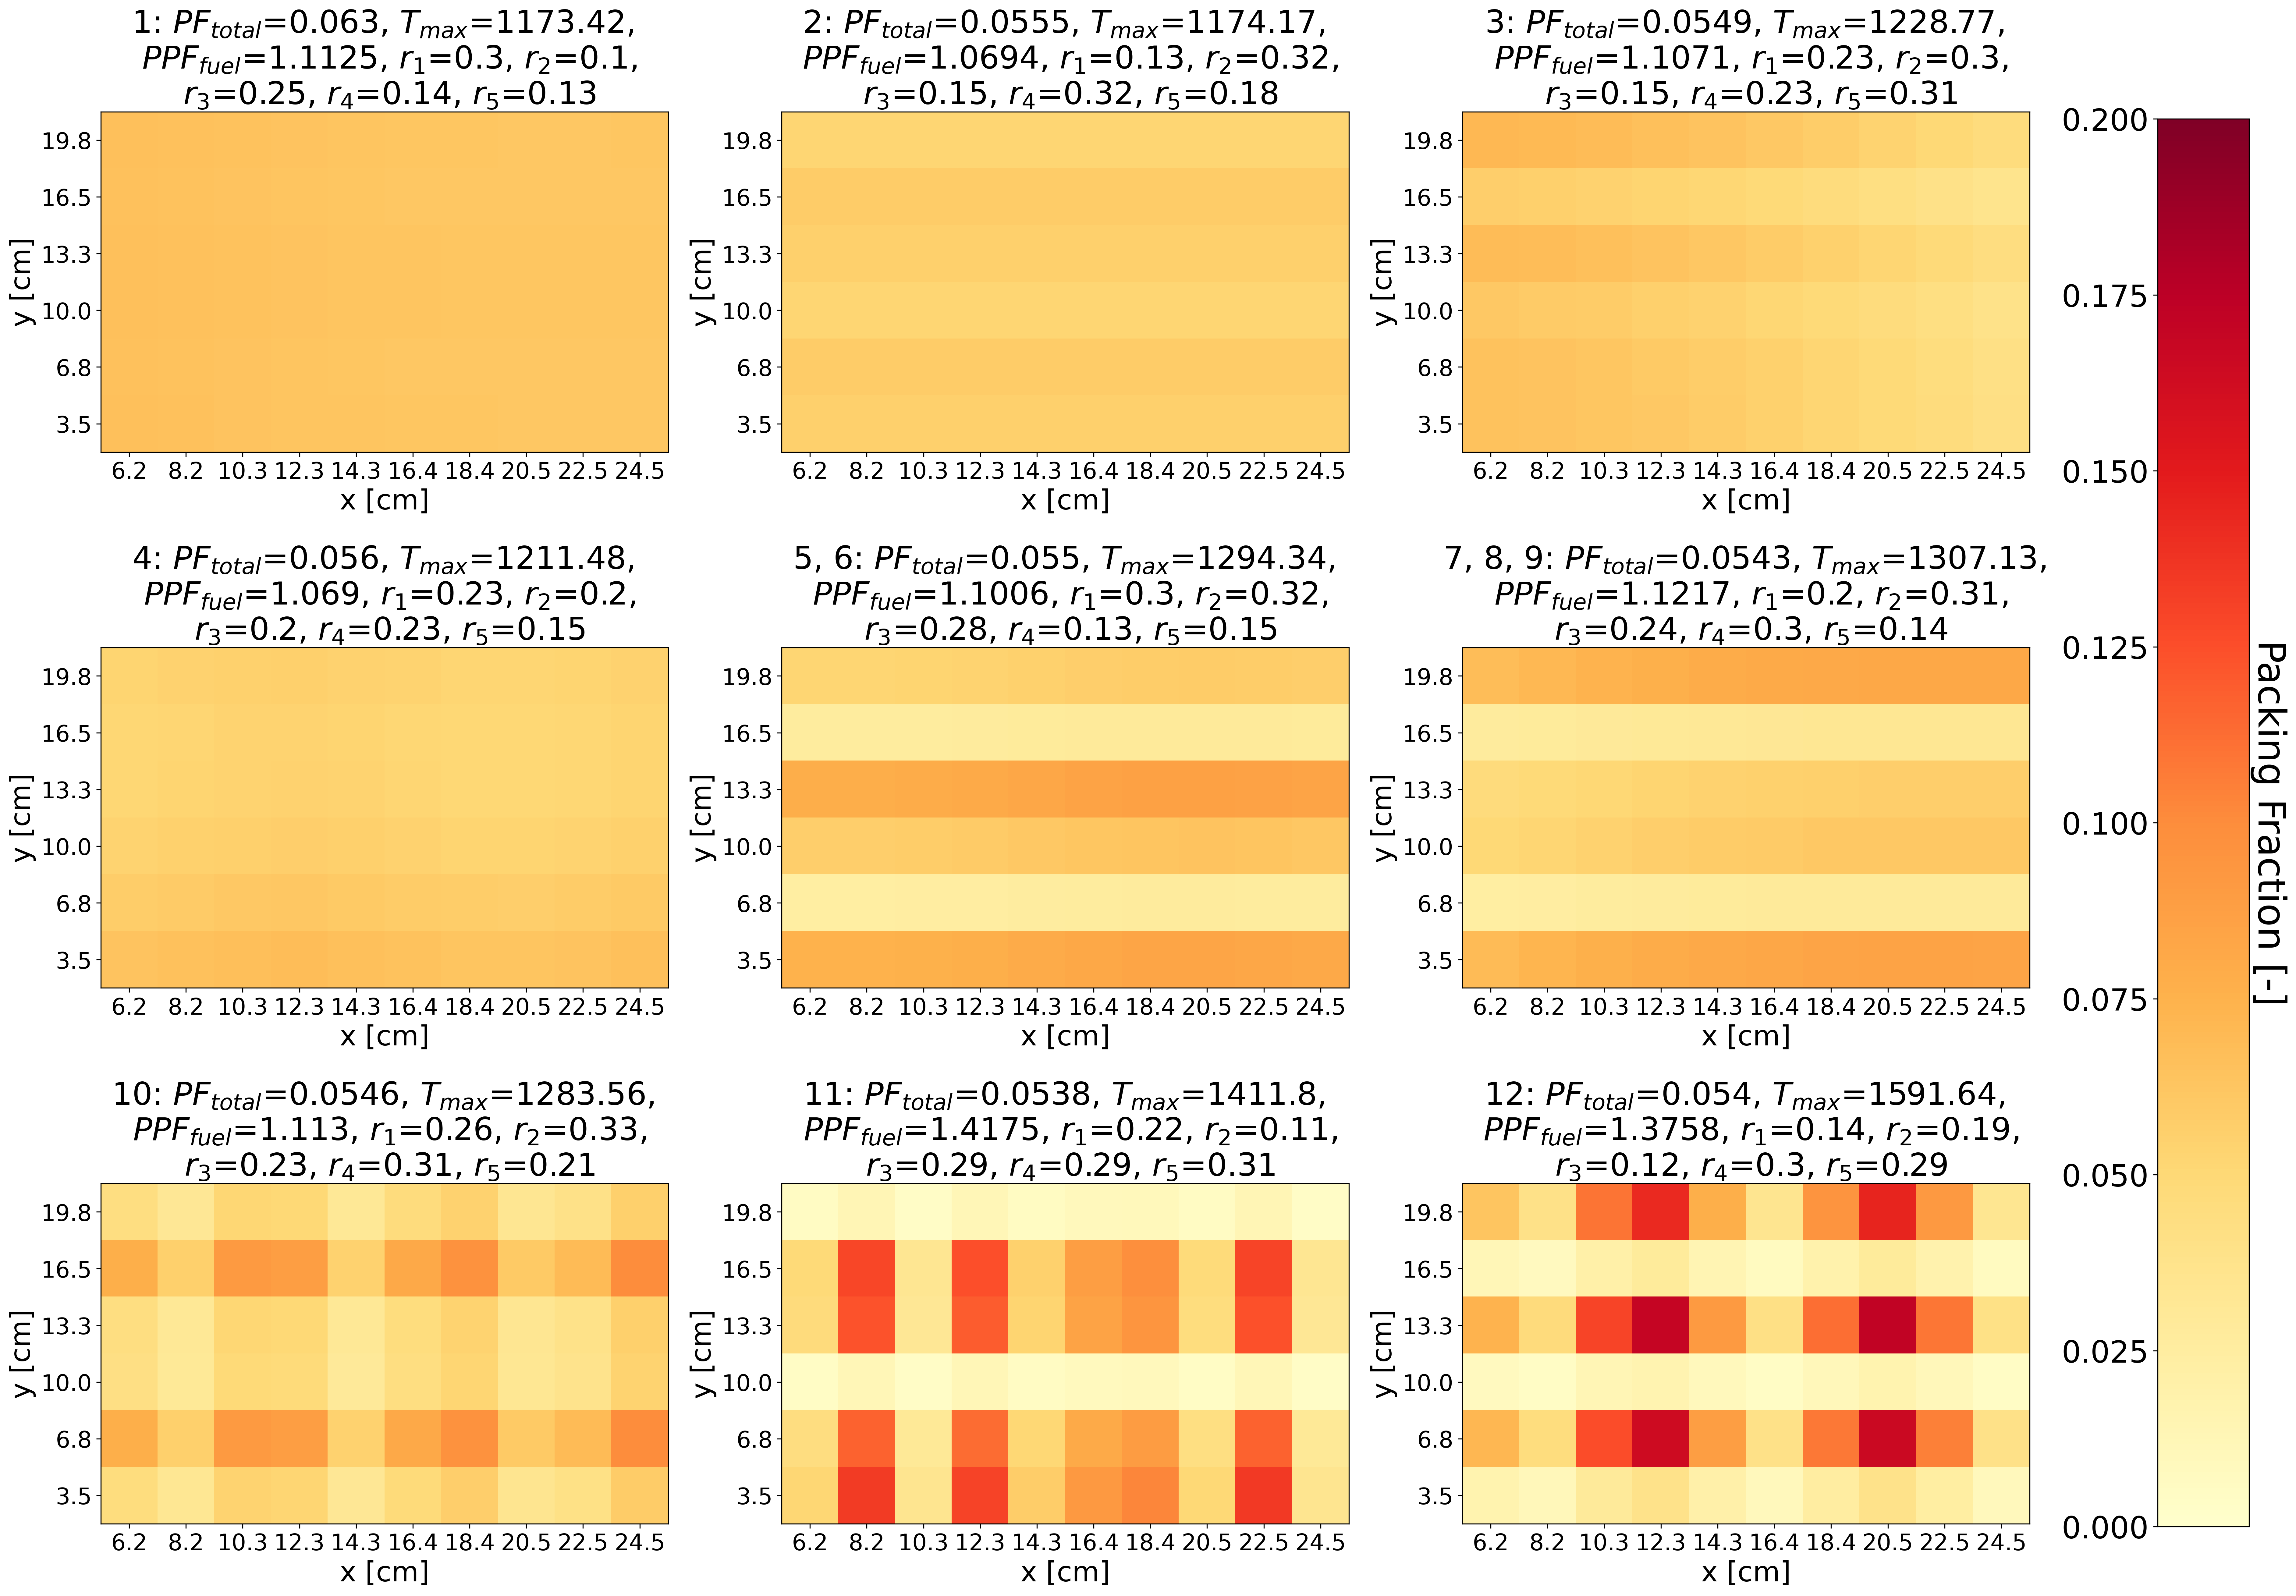
\includegraphics[width=0.8\linewidth]{../docs/figures/assem-obj-3-all-distr.png}}
        \only<2>{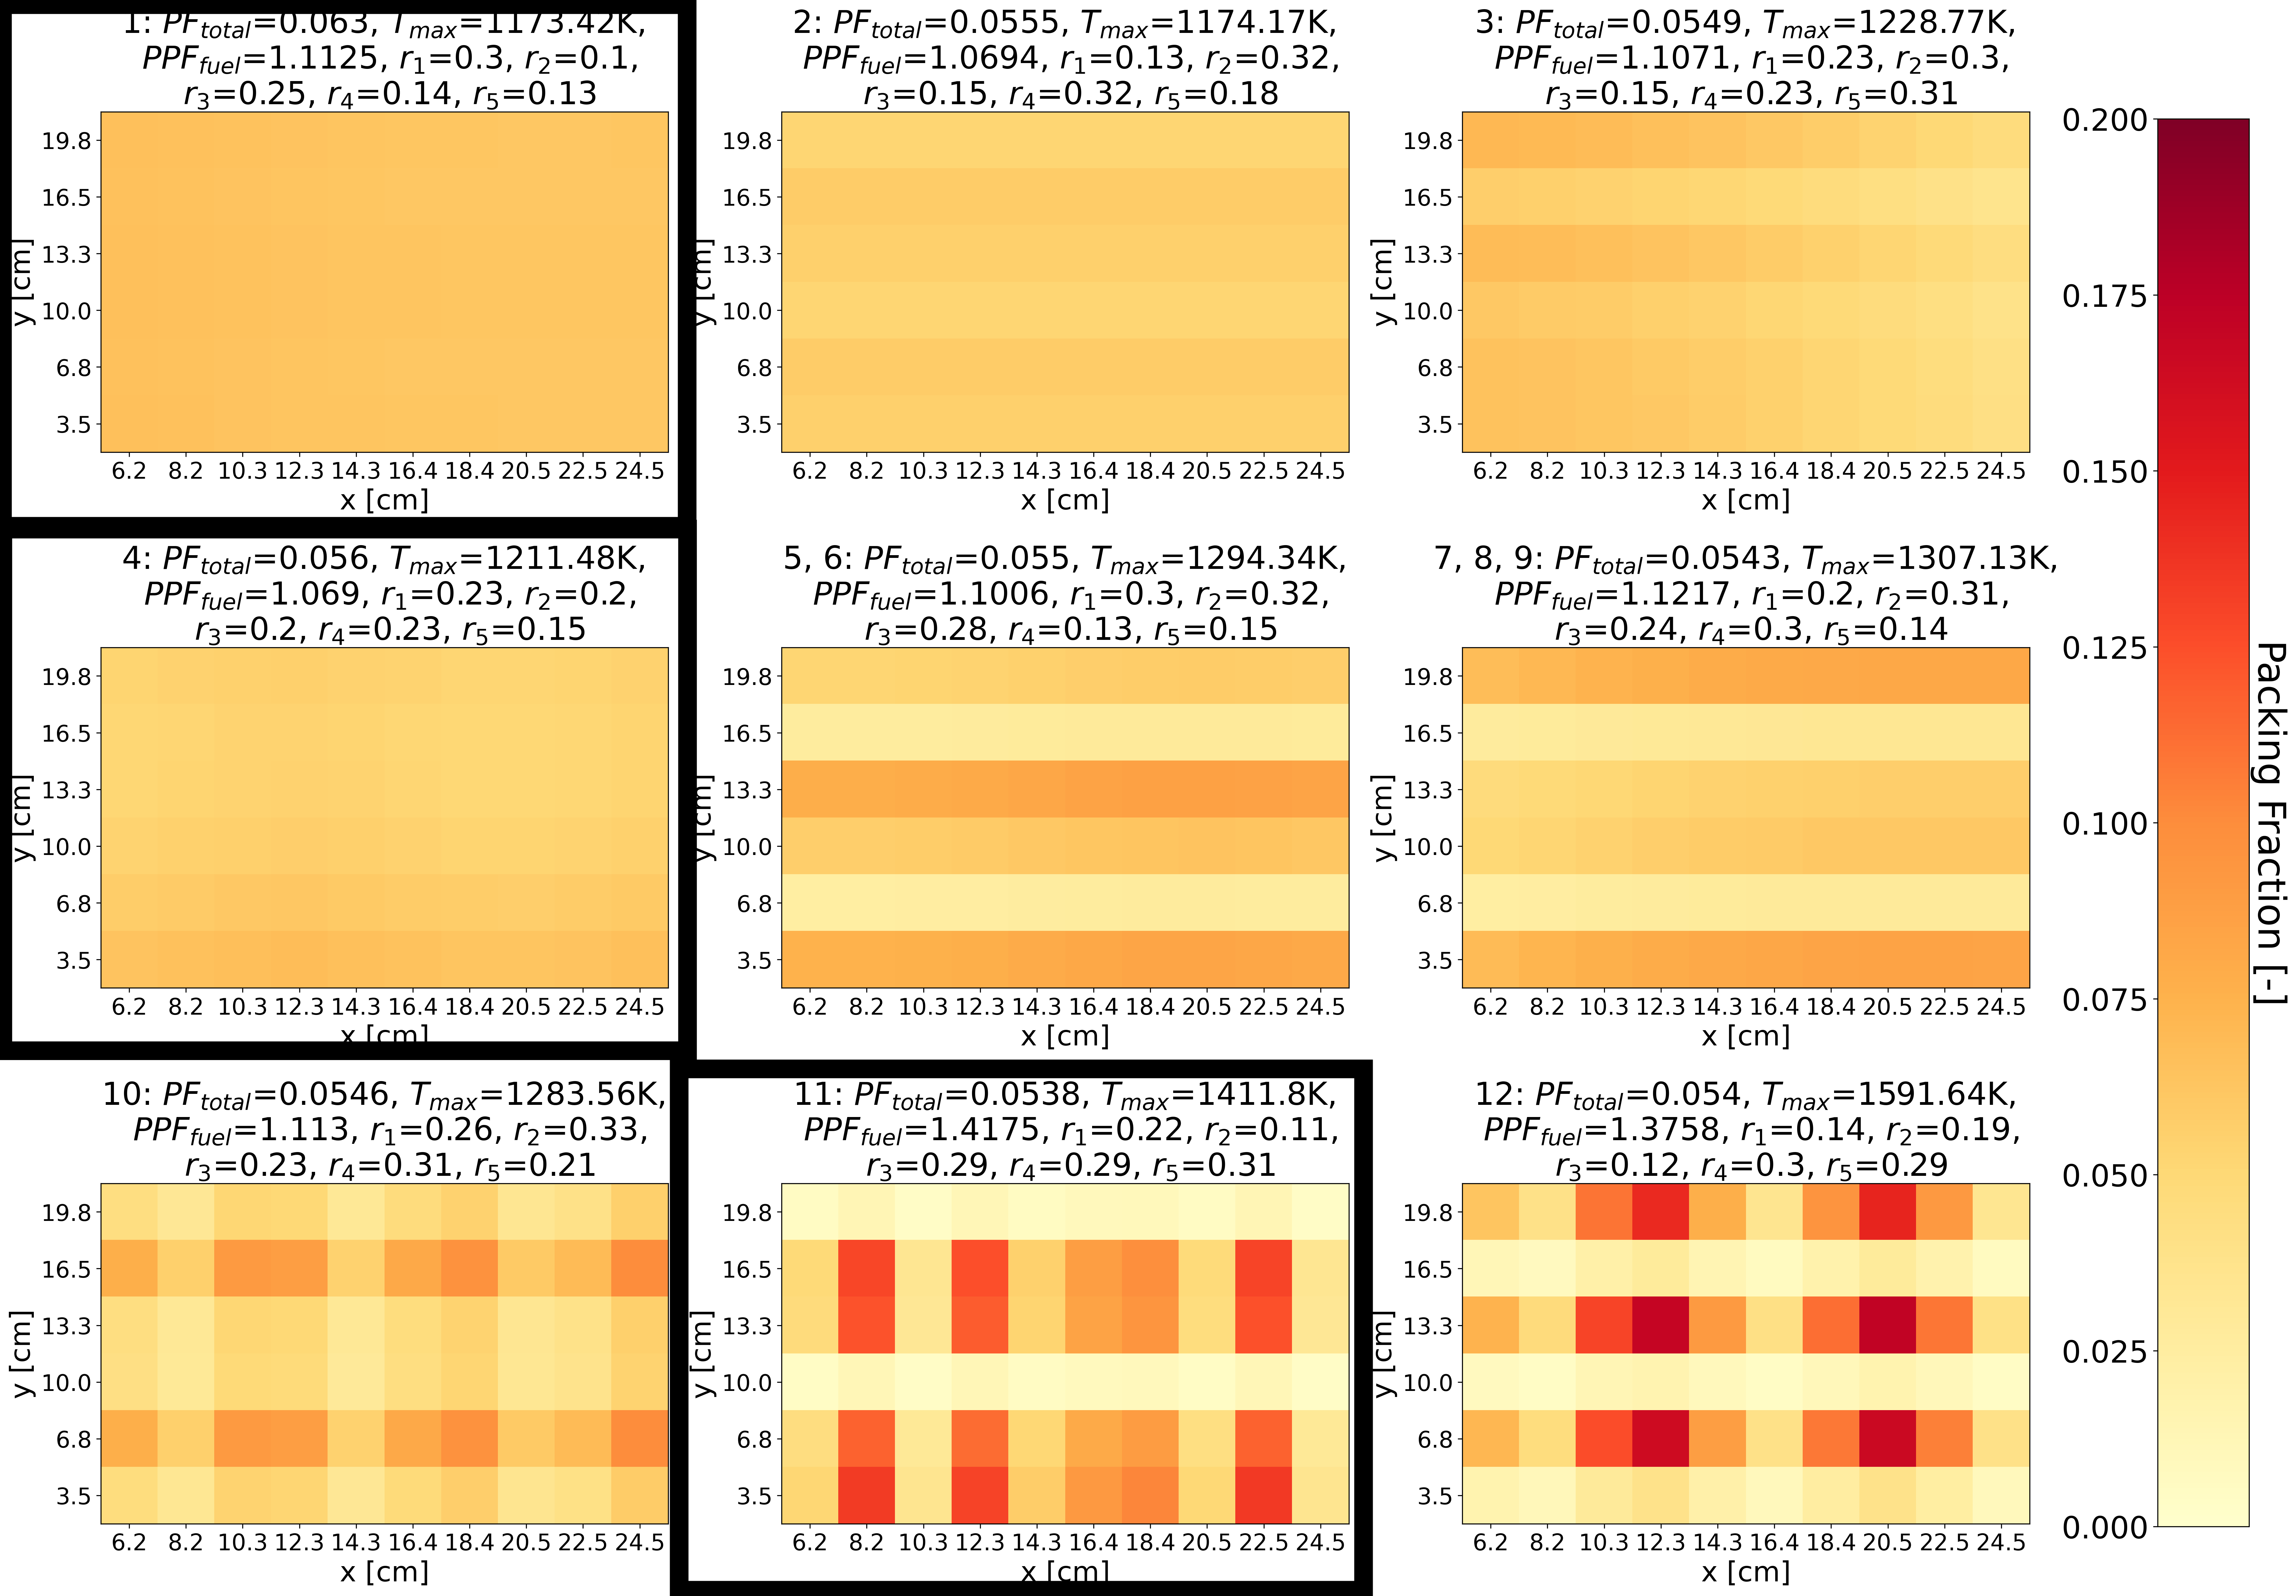
\includegraphics[width=0.8\linewidth]{figures/assem-obj-3-all-distr-annotated.png}}  
        \caption{TRISO distributions for the 12 reactor models on simulation 
        a-3b's Pareto front.}
    \end{figure}
\end{frame}

\begin{frame}
    \frametitle{AHTR One-Third Assembly Simulation a-3b Results}
    \begin{columns}
        \begin{column}{0.6\textwidth}
        \begin{figure}
            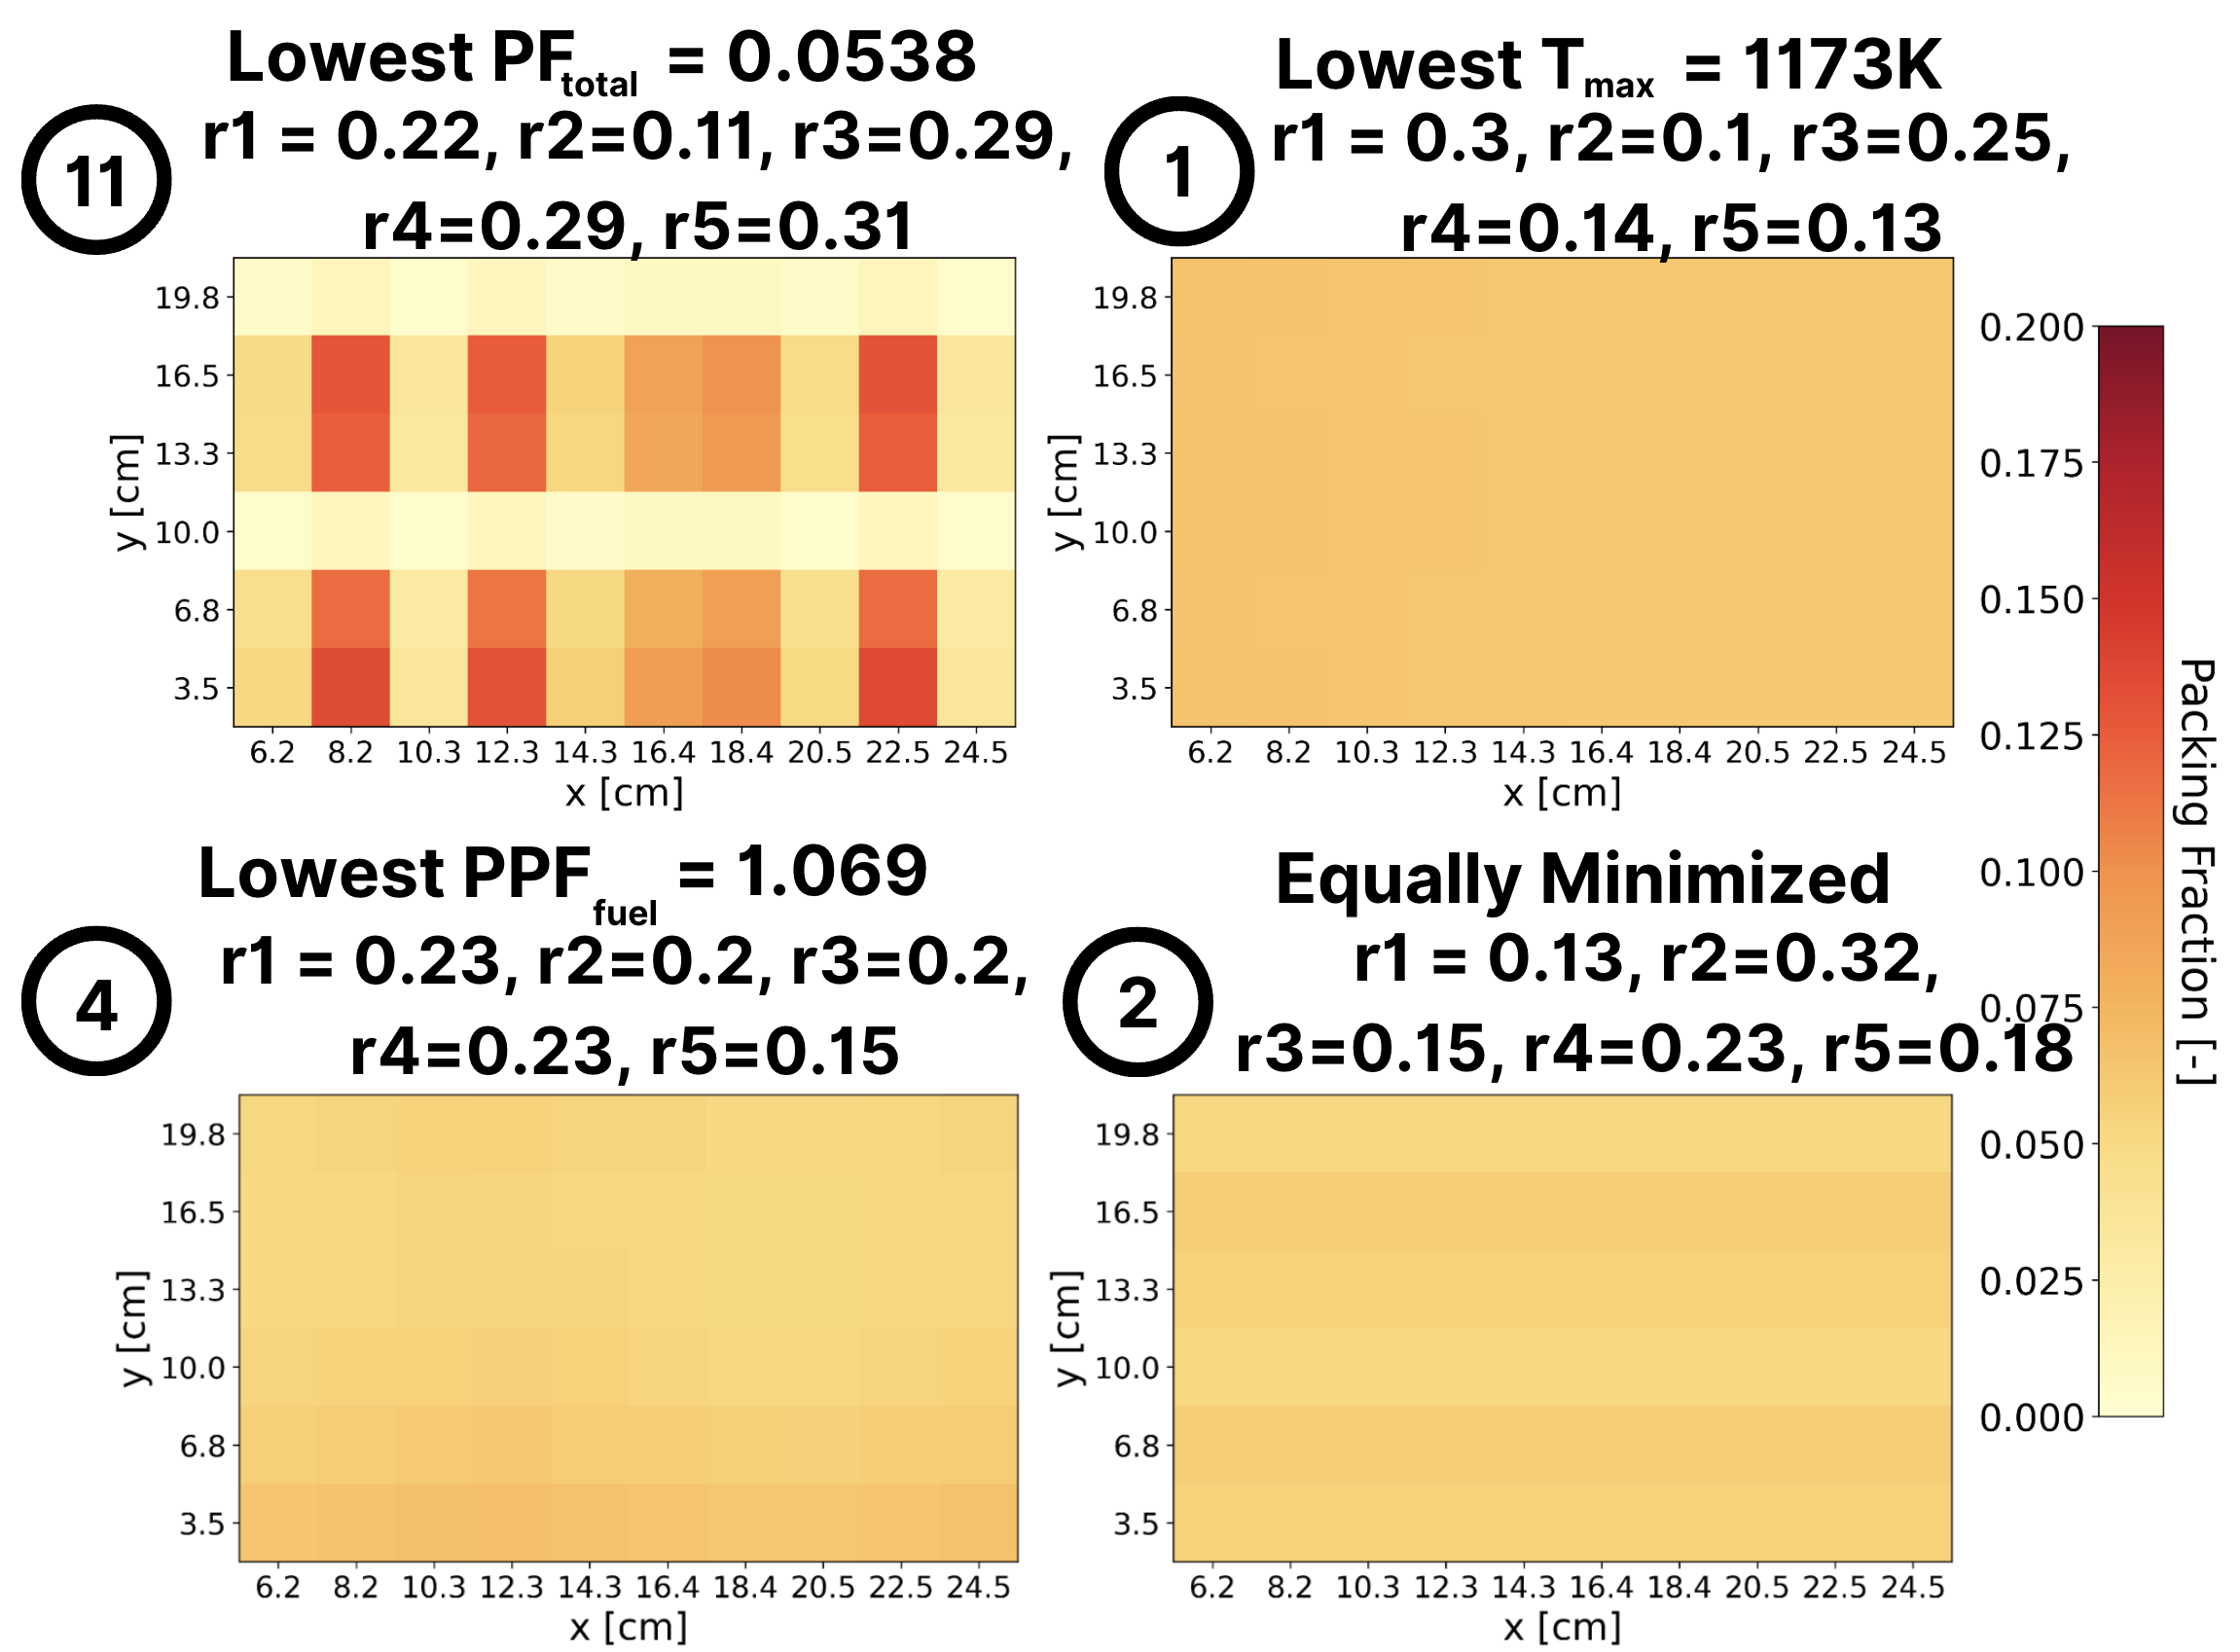
\includegraphics[width=\linewidth]{figures/a-3b-four-disr.png} 
        \end{figure}
        \end{column}
        \begin{column}{0.4\textwidth}
            \textbf{Key Observations}
            \begin{itemize}
                \item TRISO distribution flatness is influenced by minimize $T_{max}$
                objective 
                \item Variations in TRISO distributions are influenced by minimize 
                $PF_{total}$ and $PPF_{fuel}$ objectives 
                \item Larger radius values are observed near temperature peaks 
            \end{itemize}
        \end{column}
        \end{columns}
\end{frame}

\begin{frame}
    \frametitle{AHTR One-Third Assembly Simulation a-3b Results}
    \textbf{Simulation a-3b: One-third assembly model that equally minimized all 
    objectives (reactor model 2).}

    \begin{figure}
        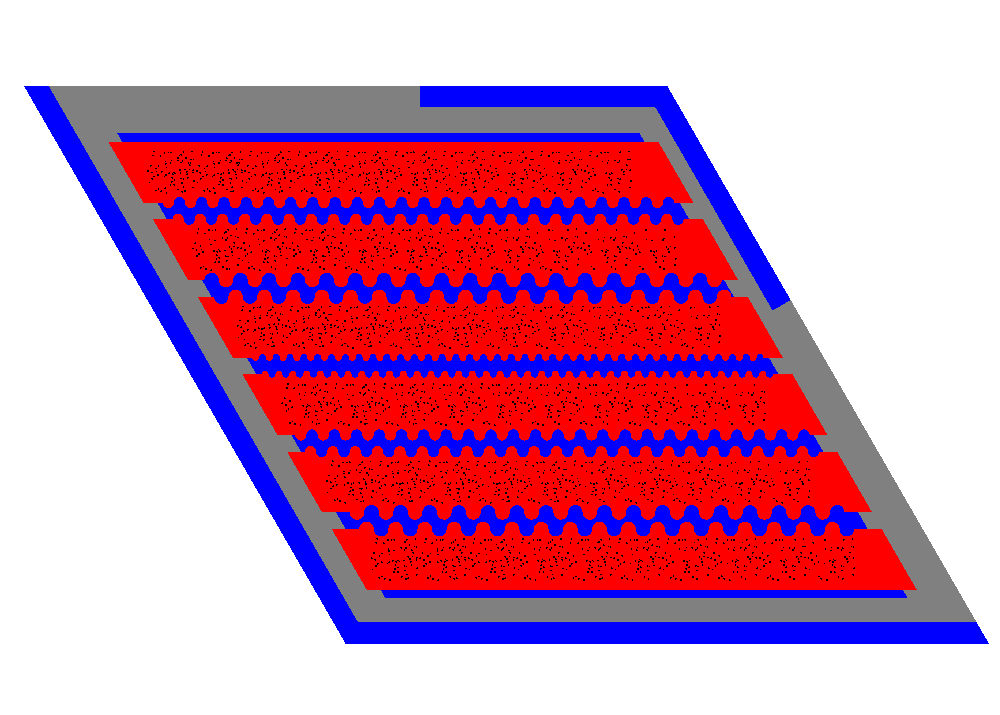
\includegraphics[width=0.75\linewidth]{../docs/figures/assem-obj-3-all-min-all.png} 
    \end{figure}
\end{frame}

\begin{frame}
    \frametitle{Multi-Objective Optimization Major Takeaways}
    The multi-objective optimization simulations successfully explored the large 
    design space by finding \textbf{wide spread of reactor models on their 
    Pareto fronts}. 

    \vspace{0.2cm}
    The reactor models on the Pareto fronts have \textbf{different $PF_{total}$, 
    TRISO distributions, and coolant channel shapes}, depending on the extent 
    each objective is minimized due to the nature of multi-objective
    optimization that results in a \textbf{tradeoff between objectives}. 

    \vspace{0.3cm}
    \textbf{Minimize $T_{max}$ objective} 
    \begin{itemize}
        \item Continues to flatten TRISO distribution 
        \item Maximize radius values of FliBe channels located near temperature peaks
        \item TRISO distribution has a larger impact on $T_{max}$ than coolant channel 
        shape  
    \end{itemize}

    \textbf{Minimize $PF_{total}$ and $PPF_{fuel}$} 
    \begin{itemize}
    \item These two objectives influence each other to have unexpected TRISO
    distributions at different $PF_{total}$ values
    \end{itemize} 

\end{frame}

\begin{frame}
    \frametitle{ROLLO Tool + AHTR Optimization Simulations: Summary}
    \visible<1->{\begin{block}{I Successfully Completed AHTR Optimization for Non-conventional Designs
    Research Objectives}
    \begin{itemize}
        \item I developed \acrfull{ROLLO} tool that enables generative reactor design
        optimization with evolutionary algorithms 
        \item I demonstrated ROLLO's application on AHTR optimization for spatially variant 
        fuel distributions and wavy coolant channels
    \end{itemize}    
    \end{block}}
    \visible<2->{\begin{block}{Major Takeaways}
        \begin{itemize}
            \item Results demonstrate ROLLO's success in conducting a multi-objective 
            global search of the large AHTR design space to find optimal reactor models 
            that satisfy all the objectives
            \item Once the ROLLO search is complete, reactor designers gain a better 
            intuition of the model's reactor physics and can view the narrower reactor 
            design space that meets their defined objectives
        \end{itemize}
    \end{block}}
\end{frame}